\documentclass[11pt,a4paper]{article}
\usepackage[margin=1.8cm,top=2.5cm,bottom=2.2cm,headheight=24pt]{geometry}
\usepackage{fontspec}
\setmainfont{RakutenSerifApp}[
  Path = /home/sudheesh/.fonts/Notesnook/,
  Extension = .ttf,
  UprightFont = *-Regular,
  BoldFont = *-Bold,
  ItalicFont = *-Italic,
  BoldItalicFont = *-BoldItalic
]
\usepackage{amsmath,amssymb,mathtools}
\usepackage{booktabs,array,tabularx,multirow}
\usepackage{graphicx}
\graphicspath{{figures_mod3/}}
\usepackage{xcolor}
\usepackage{titlesec}
\usepackage{fancyhdr}
\usepackage{enumitem}
\usepackage{caption}
\usepackage{tcolorbox}
\tcbuselibrary{skins,breakable}
\usepackage{tikz}
\usepackage{pgfplots}
\pgfplotsset{compat=1.18}
\usetikzlibrary{arrows.meta,calc,positioning,patterns,decorations.pathmorphing}
\usepackage[hidelinks,pdfusetitle]{hyperref}

% Define custom column for tabularx
\newcolumntype{Y}{>{\centering\arraybackslash}X}

% Define color palette
\definecolor{navyprimary}{RGB}{15, 35, 65}
\definecolor{accentblue}{RGB}{2, 132, 199}
\definecolor{tealaccent}{RGB}{13, 148, 136}
\definecolor{cardbg}{RGB}{248, 250, 252}
\definecolor{cardborder}{RGB}{203, 213, 225}
\definecolor{calloutbg}{RGB}{241, 245, 249}
\definecolor{calloutframe}{RGB}{100, 116, 139}
\definecolor{formulabg}{RGB}{238, 242, 255}
\definecolor{formulaframe}{RGB}{99, 102, 241}
\definecolor{examplebg}{RGB}{250, 250, 250}
\definecolor{exampleframe}{RGB}{56, 189, 248}
\definecolor{highlightgold}{RGB}{180, 83, 9}
\definecolor{alertbg}{RGB}{254, 242, 242}
\definecolor{alertframe}{RGB}{239, 68, 68}

% Caption styling
\captionsetup{font=small,labelfont={bf,color=navyprimary},skip=5pt}

% Typography & Header/Footer
\pagestyle{fancy}
\fancyhf{}
\renewcommand{\headrulewidth}{0.6pt}
\renewcommand{\headrule}{\hbox to\headwidth{\color{navyprimary}\leaders\hrule height \headrulewidth\hfill}}
\fancyhead[L]{\small\bfseries\color{navyprimary}Power Electronics (Module 3) --- Master Study Guide}
\fancyhead[R]{\small\color{accentblue}CET S5 EEE}
\fancyfoot[L]{\small\color{gray}College of Engineering Trivandrum}
\fancyfoot[R]{\small\bfseries\color{navyprimary}Page \thepage}

% Section Titles Styling
\titleformat{\section}{\Large\bfseries\color{navyprimary}}{}{0em}{}[\vspace{1mm}{\color{accentblue}\hrule height 1.2pt}]
\titleformat{\subsection}{\large\bfseries\color{accentblue}}{}{0em}{}
\titleformat{\subsubsection}{\normalsize\bfseries\color{tealaccent}}{}{0em}{}

% Tcolorbox custom environments (Border-free modern cards with solid background colors)
\newtcolorbox{conceptbox}[1][]{
  enhanced,
  colback=calloutbg,
  colframe=calloutbg,
  colbacktitle=calloutbg,
  coltitle=navyprimary,
  fonttitle=\bfseries,
  title={#1},
  titlerule=0pt,
  boxrule=0pt,
  frame hidden,
  arc=2.5mm,
  left=4mm, right=4mm, top=3mm, bottom=3mm,
  breakable
}

\newtcolorbox{formulabox}[1][]{
  enhanced,
  colback=formulabg,
  colframe=formulabg,
  colbacktitle=formulabg,
  coltitle=navyprimary,
  fonttitle=\bfseries,
  title={#1},
  titlerule=0pt,
  boxrule=0pt,
  frame hidden,
  arc=2.5mm,
  left=4mm, right=4mm, top=3mm, bottom=3mm,
  breakable
}

\newtcolorbox{examplebox}[1][]{
  enhanced,
  colback=examplebg,
  colframe=examplebg,
  colbacktitle=examplebg,
  coltitle=navyprimary,
  fonttitle=\bfseries,
  title={#1},
  titlerule=0pt,
  boxrule=0pt,
  frame hidden,
  arc=2.5mm,
  left=4mm, right=4mm, top=3mm, bottom=3mm,
  middle=2.5mm,
  segmentation style={solid, draw=cardborder, line width=0.6pt},
  breakable
}

\newtcolorbox{alertbox}[1][]{
  enhanced,
  colback=alertbg,
  colframe=alertbg,
  colbacktitle=alertbg,
  coltitle=alertframe,
  fonttitle=\bfseries,
  title={#1},
  titlerule=0pt,
  boxrule=0pt,
  frame hidden,
  arc=2.5mm,
  left=4mm, right=4mm, top=3mm, bottom=3mm,
  breakable
}

% Remove boxed black borders
\renewcommand{\boxed}[1]{#1}

\begin{document}

% Title Block
\begin{center}
  {\LARGE\bfseries\color{navyprimary}POWER ELECTRONICS}\\[2mm]
  {\Large\bfseries\color{accentblue}Module 3: AC Voltage Controllers, DC-AC Inverters \& Utility Interface}\\[3mm]
  {\normalsize\bfseries B.Tech S5 Electrical \& Electronics Engineering (EEE) $\cdot$ APJ Abdul Kalam Technological University}\\[1mm]
  {\small\color{gray}Comprehensive Master Study Guide \& University Examination Preparation Manual}\\[2mm]
  \noindent\makebox[\linewidth]{\color{navyprimary}\rule{\linewidth}{1.5pt}}
\end{center}

\vspace{-2mm}
\tableofcontents
\vspace{4mm}
\noindent\makebox[\linewidth]{\color{cardborder}\rule{\linewidth}{0.6pt}}
\vspace{2mm}

\section{AC Voltage Controllers (ACVC) / AC Regulators}

\subsection{Foundational Principles and Classification}

An \textbf{AC Voltage Controller} (also termed an \textbf{AC Voltage Regulator}) is a line-frequency phase-controlled or integral-cycle switched converter that converts a fixed-voltage, fixed-frequency alternating current supply into a \textbf{variable-voltage, fixed-frequency AC output} without an intermediate DC stage:
\begin{equation}
\text{Fixed AC Input } (V_s, f) \xrightarrow{\text{AC Voltage Controller}} \text{Variable AC Output } (V_{or}, f)
\end{equation}
Because conversion is accomplished entirely in a single stage using line-commutated thyristors or TRIACs, AC voltage controllers feature extremely high operational efficiency ($\eta > 98\%$), rugged mechanical simplicity, low initial cost, and the complete absence of bulky reactive filter banks.

\subsubsection{Classification of AC Voltage Control Methods}
AC voltage controllers are categorized into three distinct operational methodologies according to the switching mechanism employed (frequently evaluated in university examinations):

\begin{enumerate}[leftmargin=*]
  \item \textbf{Phase Angle Control (PAC):}
  \begin{itemize}[leftmargin=*]
    \item \textbf{Mechanism:} The power semiconductor switches (a pair of anti-parallel SCRs or a TRIAC) connect the load to the AC source for a controllable fraction of each supply half-cycle. Conduction is initiated at a controllable delay angle $\alpha$ (measured relative to the zero-crossing of the input supply voltage) and ceases naturally at current zero ($\beta$) via natural (line) commutation.
    \item \textbf{Advantages:} Provides continuous, smooth, instantaneous, and infinitely variable control of RMS load voltage from $0$ to $V_s$.
    \item \textbf{Disadvantages:} The abrupt chopping of sinusoidal voltage waveforms introduces substantial low-order current harmonics (3rd, 5th, 7th) and causes the supply displacement factor to lag significantly as $\alpha$ increases.
    \item \textbf{Primary Applications:} Universal motor speed control, light dimmers, induction motor soft-starters, industrial furnace heating.
  \end{itemize}

  \item \textbf{Integral Cycle Control (On-Off / Burst Firing Control):}
  \begin{itemize}[leftmargin=*]
    \item \textbf{Mechanism:} The thyristor switches connect the load to the AC mains for an integral number of complete supply cycles ($n$ cycles), and then remain un-triggered for another integral number of cycles ($m$ cycles). Switching is always synchronized to occur at the zero-crossing of the supply voltage ($v_s(t) = 0$).
    \item \textbf{Mathematical Duty Ratio and RMS Voltage:}
    \begin{equation}
    k = \frac{n}{n + m} = \frac{T_{on}}{T_o} \implies V_{or} = V_s \sqrt{k} = V_s \sqrt{\frac{n}{n + m}}
    \end{equation}
    where $T_o = (n + m)T$ is the overall repeating period.
    \item \textbf{Advantages:} Because switching transitions occur exclusively at natural voltage zero-crossings ($dv/dt \to 0$ and $di/dt \to 0$), radio frequency interference (RFI), electromagnetic interference (EMI), and switching losses are virtually zero.
    \item \textbf{Disadvantages:} Sub-harmonic frequency components (frequencies below the mains supply frequency $f$) and line flicker are introduced, making this method completely unsuitable for motor speed control or lighting systems.
    \item \textbf{Primary Applications:} Loads with very large mechanical or thermal time constants, such as industrial electric ovens, boiler heaters, and plastic extrusion mold heaters.
  \end{itemize}

  \item \textbf{Sequence Control of AC Voltage Controllers:}
  \begin{itemize}[leftmargin=*]
    \item \textbf{Mechanism:} Two or more parallel transformer-tapped stages of AC voltage controllers are fired in sequence. By controlling only one stage at a time while leaving others fully ON or fully OFF, the output voltage is varied with substantially reduced harmonic distortion and a significantly improved supply power factor across the entire operating range.
  \end{itemize}
\end{enumerate}

\begin{figure}[htbp]
\centering
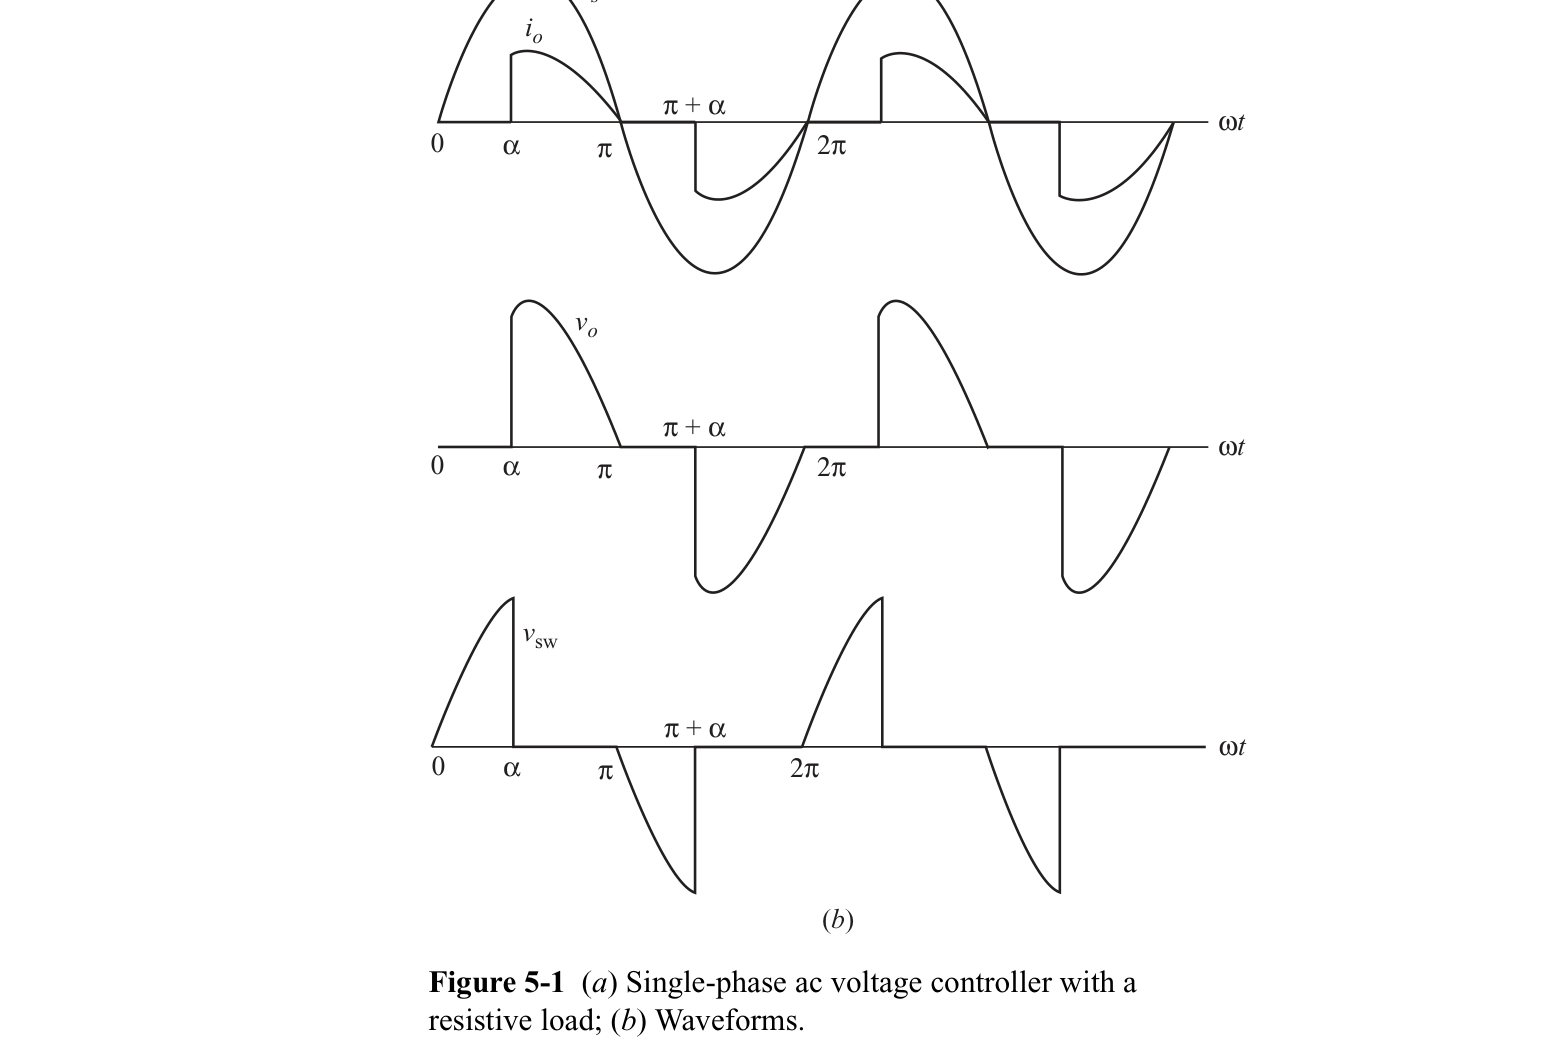
\includegraphics[width=0.65\textwidth]{hart_fig_5_1_acvc_r.png}
\caption{Single-phase full-wave AC voltage controller with resistive load: (a) Power circuit diagram using two anti-parallel thyristors $T_1$ and $T_2$; (b) Supply voltage $v_s$, gating signals $i_{g1}$ and $i_{g2}$, load voltage $v_o$, and thyristor voltage $v_{T1}$ waveforms for firing delay angle $\alpha$. (Source: Daniel W. Hart, Fig.\ 5-1)}
\label{fig:acvc_r_circuit}
\end{figure}

\subsection{Single-Phase Full-Wave AC Voltage Controller with Pure Resistive ($R$) Load}

Consider the circuit of Figure~\ref{fig:acvc_r_circuit}a supplied by a single-phase sinusoidal AC source $v_s(t) = V_m \sin(\omega t) = \sqrt{2}V_s \sin(\omega t)$. Two SCRs ($T_1$ and $T_2$) are connected in anti-parallel (back-to-back) between the AC mains and a resistive load $R$.

\subsubsection{Circuit Operation Across One Full Fundamental Cycle}
\begin{itemize}[leftmargin=*]
  \item \textbf{Positive Half-Cycle ($0 \le \omega t \le \pi$):} Supply voltage $v_s > 0$. Thyristor $T_1$ is forward-biased, while $T_2$ is reverse-biased ($v_{AK2} < 0$).
  \begin{itemize}
    \item From $\omega t = 0$ to $\omega t = \alpha$, $T_1$ remains OFF. No current flows ($i_o = 0$), load voltage $v_o = 0$, and the full line voltage appears across $T_1$ ($v_{T1} = v_s$).
    \item At $\omega t = \alpha$, a firing pulse is applied to the gate of $T_1$. $T_1$ turns ON instantaneously.
    \item From $\omega t = \alpha$ to $\pi$, $T_1$ conducts load current:
    \begin{equation}
    v_o(t) = v_s(t) = V_m \sin(\omega t), \quad i_o(t) = \frac{v_s(t)}{R} = \frac{V_m}{R}\sin(\omega t)
    \end{equation}
    \item At $\omega t = \pi$, the supply voltage reverses polarity. The current through $T_1$ drops naturally to zero ($i_o(\pi) = 0$), turning $T_1$ OFF via natural (line) commutation.
  \end{itemize}

  \item \textbf{Negative Half-Cycle ($\pi \le \omega t \le 2\pi$):} Supply voltage $v_s < 0$. Thyristor $T_2$ is forward-biased, while $T_1$ is reverse-biased.
  \begin{itemize}
    \item At $\omega t = \pi + \alpha$, a firing pulse is applied to the gate of $T_2$. $T_2$ turns ON.
    \item From $\omega t = \pi + \alpha$ to $2\pi$, $T_2$ conducts negative load current:
    \begin{equation}
    v_o(t) = v_s(t) = V_m \sin(\omega t), \quad i_o(t) = \frac{V_m}{R}\sin(\omega t) \quad (< 0)
    \end{equation}
    \item At $\omega t = 2\pi$, $i_o(2\pi) = 0$, and $T_2$ turns OFF naturally.
  \end{itemize}
\end{itemize}

\subsubsection{Rigorous Mathematical Derivation of RMS Output Voltage}
Because the output voltage waveform exhibits half-wave symmetry ($v_o(\omega t + \pi) = -v_o(\omega t)$), the root-mean-square (RMS) value can be computed over a half-cycle ($0$ to $\pi$):
\begin{align}
V_{or} &= \sqrt{\frac{1}{\pi} \int_{\alpha}^{\pi} \left[V_m \sin(\omega t)\right]^2 d(\omega t)} = \sqrt{\frac{V_m^2}{\pi} \int_{\alpha}^{\pi} \frac{1 - \cos(2\omega t)}{2} d(\omega t)} \notag\\
&= \sqrt{\frac{V_m^2}{2\pi} \left[ \omega t - \frac{\sin(2\omega t)}{2} \right]_{\alpha}^{\pi}} = \sqrt{\frac{V_m^2}{2\pi} \left[ (\pi - \alpha) - \left(\frac{\sin(2\pi) - \sin(2\alpha)}{2}\right) \right]} \notag\\
&= \sqrt{\frac{V_m^2}{2\pi} \left[ (\pi - \alpha) + \frac{\sin(2\alpha)}{2} \right]} = \frac{V_m}{\sqrt{2}} \sqrt{\frac{1}{\pi} \left[ (\pi - \alpha) + \frac{\sin(2\alpha)}{2} \right]}
\end{align}
Recognizing that $V_s = V_m / \sqrt{2}$ is the RMS value of the input source:
\begin{formulabox}[Master Equation: RMS Output Voltage ($R$ Load)]
\begin{equation}
V_{or} = V_s \sqrt{1 - \frac{\alpha}{\pi} + \frac{\sin(2\alpha)}{2\pi}}
\label{eq:acvc_rms_r}
\end{equation}
\end{formulabox}

\subsubsection{Performance Characteristics with $R$ Load}
\begin{itemize}[leftmargin=*]
  \item \textbf{RMS Load Current:} $I_{or} = \frac{V_{or}}{R} = \frac{V_s}{R} \sqrt{1 - \frac{\alpha}{\pi} + \frac{\sin(2\alpha)}{2\pi}}$.
  \item \textbf{Average and RMS Thyristor Currents:} Each thyristor conducts for only one half of the symmetrical period:
  \begin{equation}
  I_{T(avg)} = \frac{1}{2\pi} \int_{\alpha}^{\pi} \frac{V_m}{R}\sin(\omega t) d(\omega t) = \frac{V_m}{2\pi R} (1 + \cos\alpha) = \frac{\sqrt{2}V_s}{2\pi R}(1 + \cos\alpha)
  \end{equation}
  \begin{equation}
  I_{T(rms)} = \frac{I_{or}}{\sqrt{2}} = \frac{V_s}{\sqrt{2}R} \sqrt{1 - \frac{\alpha}{\pi} + \frac{\sin(2\alpha)}{2\pi}}
  \end{equation}
  \item \textbf{Input Power Factor (PF):} Since input current $i_s(t) = i_o(t)$, the apparent power supplied by the mains is $S = V_s I_{or}$. The active power dissipated in the load is $P_o = I_{or}^2 R = \frac{V_{or}^2}{R}$.
  \begin{equation}
  \text{PF} = \frac{P_o}{S} = \frac{V_{or}^2 / R}{V_s I_{or}} = \frac{V_{or} I_{or}}{V_s I_{or}} = \frac{V_{or}}{V_s} = \sqrt{1 - \frac{\alpha}{\pi} + \frac{\sin(2\alpha)}{2\pi}}
  \end{equation}
  \item \textbf{Control Range:} As $\alpha$ varies from $0$ to $\pi$ ($180^\circ$):
  \begin{itemize}
    \item At $\alpha = 0$: $V_{or} = V_s$, $\text{PF} = 1.0$ (Full sinusoidal conduction).
    \item At $\alpha = \pi/2$ ($90^\circ$): $V_{or} = V_s / \sqrt{2} \approx 0.707 V_s$, $\text{PF} \approx 0.707$.
    \item At $\alpha = \pi$ ($180^\circ$): $V_{or} = 0$, $\text{PF} = 0$ (Output completely blocked).
  \end{itemize}
\end{itemize}

\subsection{Single-Phase Full-Wave AC Voltage Controller with $RL$ Load}

When the load consists of an inductive impedance $Z = \sqrt{R^2 + (\omega L)^2}$ with characteristic load impedance angle $\phi = \arctan\left(\frac{\omega L}{R}\right)$, the inductance opposes sudden changes in load current. Consequently, \textbf{the current continues to flow after the source voltage reverses polarity at $\omega t = \pi$}.

\begin{figure}[htbp]
\centering
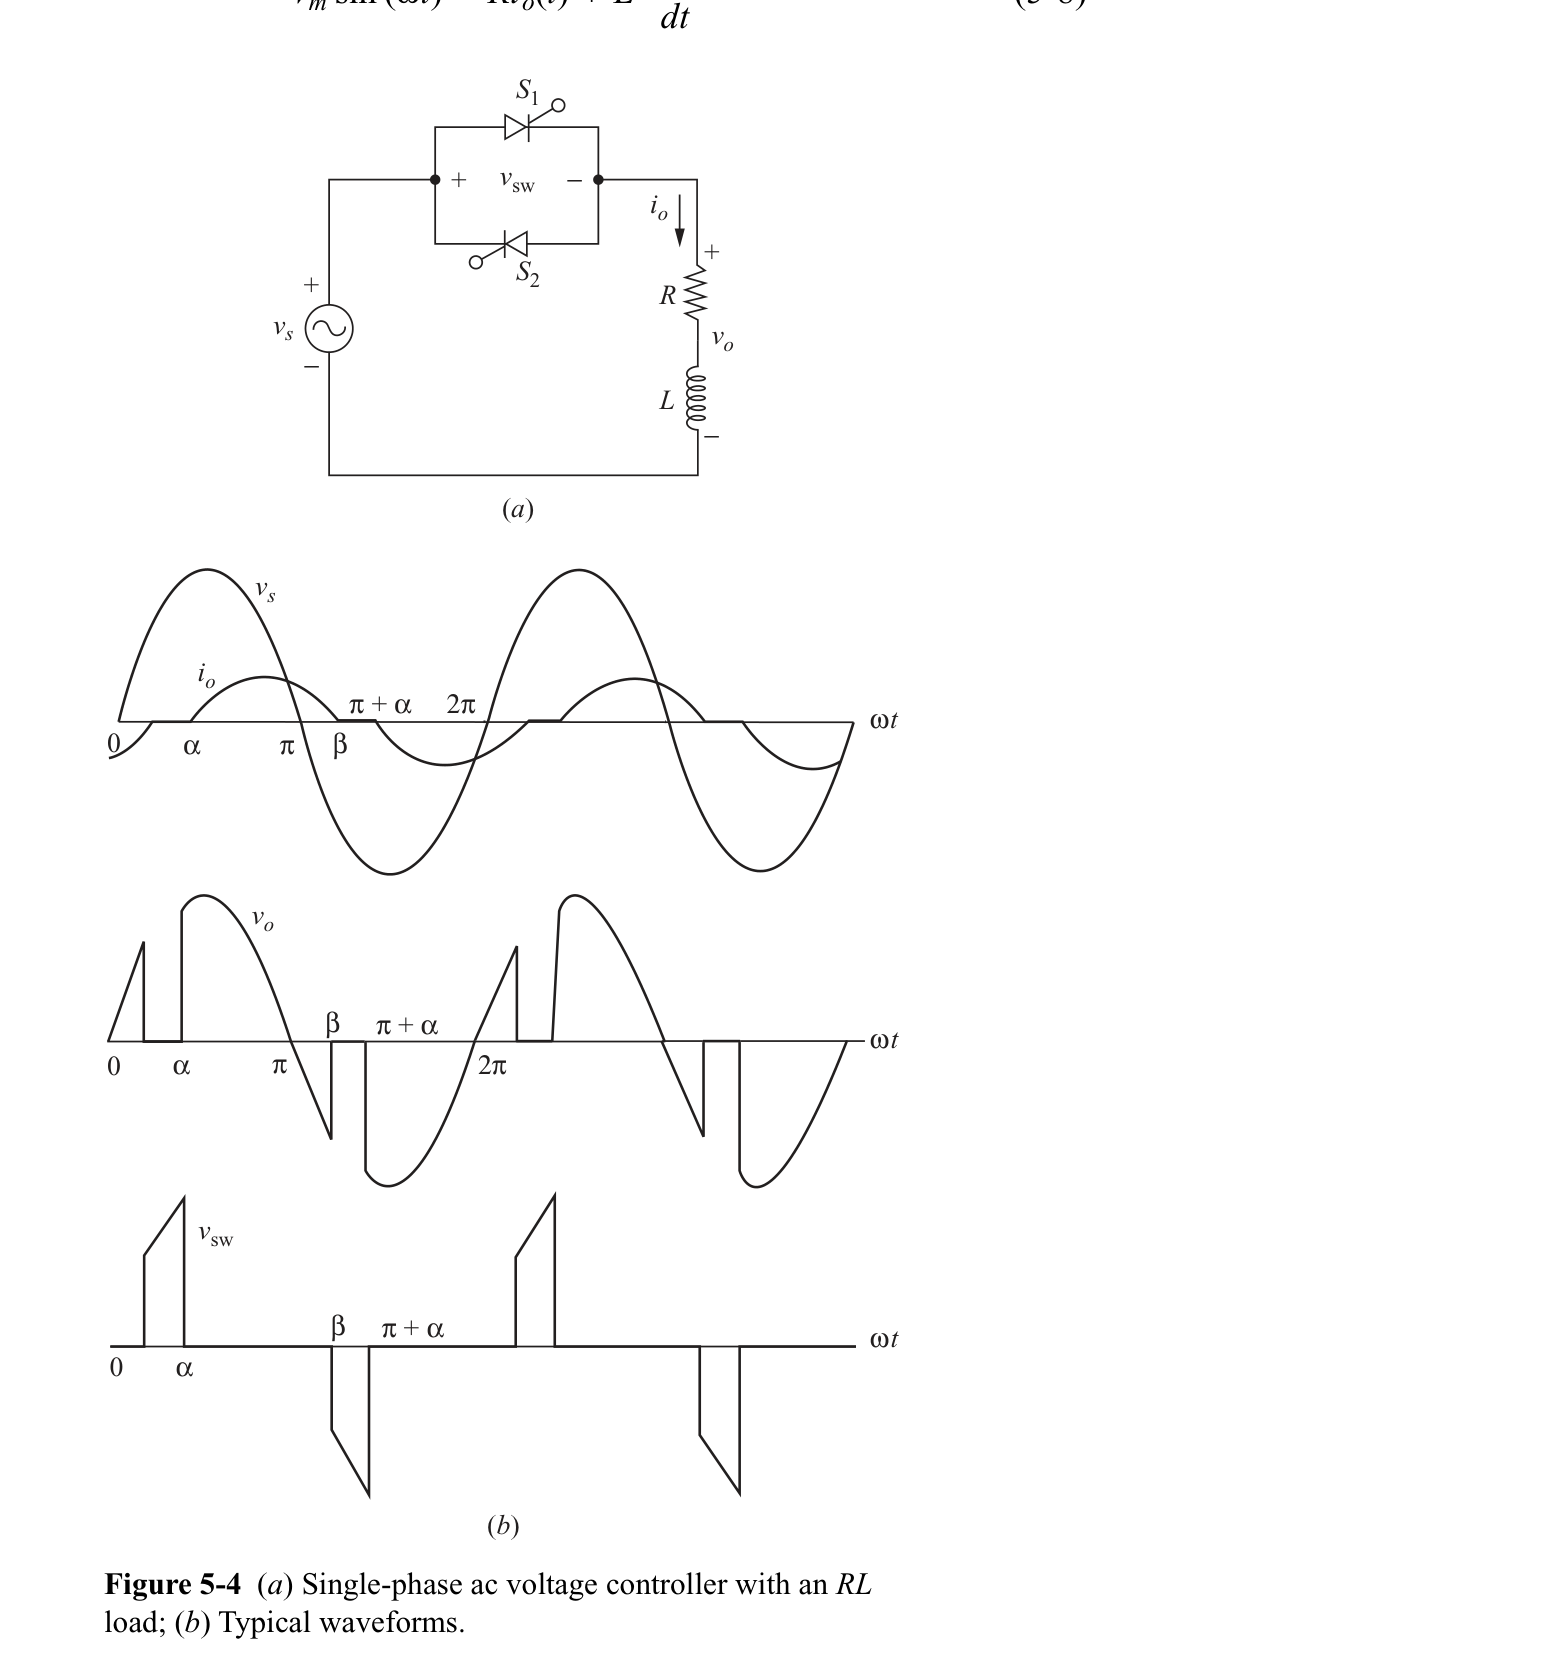
\includegraphics[width=0.68\textwidth]{hart_fig_5_4_acvc_rl.png}
\caption{Single-phase AC voltage controller with $RL$ load: Waveforms of input voltage $v_s$, thyristor gating pulses, output voltage $v_o$, and inductive load current $i_o(\omega t)$ showing the extinction angle $\beta$ and conduction angle $\gamma = \beta - \alpha$. (Source: Daniel W. Hart, Fig.\ 5-4)}
\label{fig:acvc_rl_waveforms}
\end{figure}

\subsubsection{Derivation of the Load Current Differential Equation}
During the conduction of thyristor $T_1$ ($\alpha \le \omega t \le \beta$), the governing Kirchhoff's Voltage Law (KVL) differential equation is:
\begin{equation}
L \frac{di_o(t)}{dt} + R i_o(t) = v_s(t) = V_m \sin(\omega t)
\end{equation}
The total solution consists of a steady-state particular solution $i_{ss}(t)$ and a transient complementary solution $i_{tr}(t)$:
\begin{equation}
i_o(\omega t) = \frac{V_m}{Z}\sin(\omega t - \phi) + A e^{-\frac{R}{\omega L}\omega t}
\end{equation}
where $Z = \sqrt{R^2 + (\omega L)^2}$ and $\phi = \arctan(\omega L / R)$.

Applying the initial boundary condition at the firing instant: at $\omega t = \alpha$, $i_o(\alpha) = 0$:
\begin{equation}
0 = \frac{V_m}{Z}\sin(\alpha - \phi) + A e^{-\frac{R}{\omega L}\alpha} \implies A = -\frac{V_m}{Z}\sin(\alpha - \phi) e^{\frac{R}{\omega L}\alpha}
\end{equation}
Substituting $A$ back into the current expression yields the closed-form equation for the instantaneous load current:
\begin{formulabox}[Instantaneous Load Current in ACVC with $RL$ Load]
\begin{equation}
i_o(\omega t) = \frac{V_m}{Z} \left[ \sin(\omega t - \phi) - \sin(\alpha - \phi) e^{-\frac{R}{\omega L}(\omega t - \alpha)} \right], \quad \text{for } \alpha \le \omega t \le \beta
\label{eq:acvc_io_rl}
\end{equation}
\end{formulabox}

\subsubsection{Extinction Angle ($\beta$) and Conduction Angle ($\gamma$)}
At $\omega t = \beta$, the magnetic energy stored in inductor $L$ is completely dissipated into $R$, and the current extinguishes to zero ($i_o(\beta) = 0$). Setting equation~\eqref{eq:acvc_io_rl} to zero at $\omega t = \beta$ gives the transcendental equation:
\begin{equation}
\sin(\beta - \phi) = \sin(\alpha - \phi) e^{-\frac{R}{\omega L}(\beta - \alpha)}
\label{eq:acvc_beta_transcendental}
\end{equation}
The conduction angle of each thyristor is defined as $\gamma = \beta - \alpha$. Equation~\eqref{eq:acvc_beta_transcendental} can be expressed in terms of $\gamma$ as:
\begin{equation}
\sin(\alpha + \gamma - \phi) = \sin(\alpha - \phi) e^{-\frac{R}{\omega L}\gamma}
\end{equation}

\subsubsection{Three Critical Conduction Regimes Based on Firing Angle $\alpha$ vs $\phi$}
The behavior of the $RL$ AC voltage controller depends decisively on the relative relationship between the firing delay angle $\alpha$ and the load impedance phase angle $\phi$:

\begin{enumerate}[leftmargin=*]
  \item \textbf{Case 1: $\alpha > \phi$ (Discontinuous Conduction Mode --- Standard Operation):}
  \begin{itemize}
    \item The current extinguishes before the next half-cycle thyristor is triggered: $\beta < \pi + \alpha$, which means the conduction angle $\gamma = (\beta - \alpha) < \pi$.
    \item There is a finite zero-current interval between the extinction of $T_1$ and the firing of $T_2$.
    \item The output voltage is fully controllable by varying $\alpha$ between $\phi$ and $\pi$.
  \end{itemize}

  \item \textbf{Case 2: $\alpha = \phi$ (Boundary / Critical Conduction Mode):}
  \begin{itemize}
    \item Substituting $\alpha = \phi$ into equation~\eqref{eq:acvc_beta_transcendental}:
    \begin{equation}
    \sin(\beta - \phi) = \sin(0) \cdot e^{-\frac{R}{\omega L}(\beta - \phi)} = 0 \implies \beta - \phi = \pi \implies \beta = \pi + \phi = \pi + \alpha
    \end{equation}
    \item The conduction angle is exactly $\gamma = \beta - \alpha = \pi$ ($180^\circ$).
    \item Thyristor $T_1$ conducts for exactly $180^\circ$. The moment $T_1$ extinguishes at $\omega t = \pi + \alpha$, thyristor $T_2$ is triggered!
    \item The load current becomes a continuous, perfectly sinusoidal waveform: $i_o(t) = \frac{V_m}{Z}\sin(\omega t - \phi)$. The converter behaves as if the load is directly connected across the AC supply!
  \end{itemize}

  \item \textbf{Case 3: $\alpha < \phi$ (Dangerous / Loss of Control Mode):}
  \begin{itemize}
    \item If a narrow gate pulse is applied at $\alpha < \phi$, thyristor $T_1$ cannot turn ON if the previous thyristor $T_2$ is still conducting negative current!
    \item If continuous or long gate pulses are used, $T_1$ will not turn ON until $T_2$ current reaches zero at $\beta$. This effectively clamps the minimum firing angle to $\alpha_{\text{min}} = \phi$.
    \item \textbf{Critical Exam Rule:} Firing angle $\alpha$ must always satisfy $\alpha \ge \phi$. A firing angle smaller than $\phi$ does not increase the load voltage and causes a loss of independent phase control or asymmetrical DC saturation of feeding transformers!
  \end{itemize}
\end{enumerate}

\subsubsection{Derivation of RMS Output Voltage with $RL$ Load}
During the conduction interval $\alpha \le \omega t \le \beta$, the load voltage equals the supply voltage: $v_o(t) = V_m \sin(\omega t)$. Outside this interval, $v_o(t) = 0$.
\begin{align}
V_{or} &= \sqrt{\frac{1}{\pi} \int_{\alpha}^{\beta} \left[V_m \sin(\omega t)\right]^2 d(\omega t)} = \sqrt{\frac{V_m^2}{2\pi} \int_{\alpha}^{\beta} \left[1 - \cos(2\omega t)\right] d(\omega t)} \notag\\
&= \sqrt{\frac{V_m^2}{2\pi} \left[ (\beta - \alpha) - \frac{\sin(2\beta) - \sin(2\alpha)}{2} \right]}
\end{align}
In terms of $V_s = V_m / \sqrt{2}$ and conduction angle $\gamma = \beta - \alpha$:
\begin{formulabox}[Master Equation: RMS Output Voltage ($RL$ Load)]
\begin{equation}
V_{or} = V_s \sqrt{\frac{1}{\pi} \left[ (\beta - \alpha) - \frac{\sin(2\beta) - \sin(2\alpha)}{2} \right]} = V_s \sqrt{\frac{1}{\pi} \left[ \gamma - \frac{\sin(2\beta) - \sin(2\alpha)}{2} \right]}
\label{eq:acvc_rms_rl}
\end{equation}
\end{formulabox}

\subsection{Single-Phase AC Voltage Controller with Pure Inductive ($L$) Load}

For a purely inductive load ($R = 0 \implies \phi = 90^\circ = \pi/2$):
\begin{equation}
L \frac{di_o}{dt} = V_m \sin(\omega t) \implies i_o(\omega t) = \frac{V_m}{\omega L} \int_{\alpha}^{\omega t} \sin(\omega t) d(\omega t) = \frac{V_m}{\omega L} (\cos\alpha - \cos\omega t)
\end{equation}
The current extinguishes when $i_o(\beta) = 0$:
\begin{equation}
\cos\alpha - \cos\beta = 0 \implies \beta = 2\pi - \alpha
\end{equation}
The conduction angle is:
\begin{equation}
\gamma = \beta - \alpha = 2\pi - 2\alpha = 2(\pi - \alpha)
\end{equation}
\begin{itemize}[leftmargin=*]
  \item Since $\phi = \pi/2$ ($90^\circ$), the control range for $\alpha$ is restricted to $\pi/2 \le \alpha \le \pi$.
  \item At $\alpha = \pi/2$: $\beta = 2\pi - \pi/2 = 3\pi/2$, $\gamma = \pi$ ($180^\circ$). Current is continuous.
  \item At $\alpha = \pi$: $\beta = \pi$, $\gamma = 0$. No current flows.
  \item This configuration is the fundamental building block of \textbf{Thyristor-Controlled Reactors (TCR)} utilized extensively in static VAR compensators (SVC) on power transmission grids!
\end{itemize}

\subsection{Gate Firing Pulse Requirements for Inductive Loads}
With an inductive load, a standard short gate trigger pulse ($10 - 20\,\mu\text{s}$) cannot ensure reliable thyristor turn-on:
\begin{conceptbox}[Gate Firing Requirements with Inductive Loads]
Because $di/dt = v_s/L$ is restricted by the load inductance, the anode current rises slowly after triggering. If a short gate pulse ends before the anode current crosses the \textbf{latching current} ($I_L$), the thyristor will immediately turn back OFF when the gate pulse is removed!

Furthermore, due to current overlap between consecutive half-cycles, the incoming thyristor may be triggered while the outgoing thyristor is still conducting.

\textbf{Mandatory Solutions:}
\begin{enumerate}
  \item \textbf{Continuous Gate Gating:} Maintain gate current throughout the desired conduction period ($\alpha$ to $\pi$). (Drawback: High average gate power dissipation).
  \item \textbf{High-Frequency Pulse Train Gating (Carrier Frequency Modulation):} Modulate the firing signal with a $10 - 30\text{ kHz}$ pulse train generated by a 555 timer or microcontroller. This reduces gate power dissipation by $>80\%$ while allowing small, compact pulse isolation transformers!
\end{enumerate}
\end{conceptbox}

\subsection{Engineering Applications of AC Voltage Controllers}
\begin{enumerate}[leftmargin=*]
  \item \textbf{Industrial and Domestic Heating:} Closed-loop temperature regulation in resistance furnaces, kilns, soldering stations, and water heaters.
  \item \textbf{Lighting Control (Dimmers):} Theater stage lighting, architectural illumination, and incandescent lamp dimming.
  \item \textbf{AC Motor Soft Starters:} During the starting of high-power three-phase squirrel-cage induction motors, direct-on-line (DOL) starting draws $6 - 8 \times I_{\text{rated}}$, creating severe line voltage dips. By ramping $\alpha$ from $150^\circ$ down to $\phi$, starting current is limited to $2 - 3 \times I_{\text{rated}}$.
  \item \textbf{Speed Control of AC Fan and Pump Motors:} Controlling stator voltage on high-slip single-phase and three-phase induction motors provides stable variable-speed torque for centrifugal fans and water pumps.
  \item \textbf{On-Load Transformer Tap Changers:} Thyristorized tap changers switch transformer winding taps under full load without mechanical arcing, contact wear, or line interruption.
  \item \textbf{Static VAR Compensators (SVC):} Thyristor-Controlled Reactors (TCR) dynamically absorb variable inductive reactive power ($Q$) to stabilize grid voltages.
\end{enumerate}


\section{Single-Phase Switch-Mode DC-AC Voltage Source Inverters (VSI)}

\subsection{Fundamental Operating Principles and Bridge Topologies}

An \textbf{Inverter} is a power electronic converter that transforms direct current (DC) electrical energy into alternating current (AC) electrical energy at a desired, precisely regulated voltage magnitude and frequency:
\begin{equation}
\text{DC Input } (V_{dc}) \xrightarrow{\text{Inverter}} \text{AC Output } (v_o(t), f_o)
\end{equation}
In a \textbf{Voltage Source Inverter (VSI)}, the DC input source is modeled as an ideal voltage source with negligible internal impedance (stiff DC bus supported by a large electrolytic DC-link capacitor bank). The output voltage waveform is strictly determined by the switching states of the converter power semiconductors, while the output current waveform is governed by the connected load impedance.

\subsubsection{Single-Phase Half-Bridge Inverter Configuration}
The single-phase half-bridge topology (Figure~\ref{fig:half_bridge}) utilizes two fully controlled semiconductor switches ($S_1, S_2$) and a three-wire split DC supply with center-tap $O$ (established by two identical series capacitors $C_1 = C_2$, each holding $V_{dc}/2$). Two anti-parallel freewheeling diodes ($D_1, D_2$) provide a continuous path for inductive load currents.

\begin{figure}[htbp]
\centering
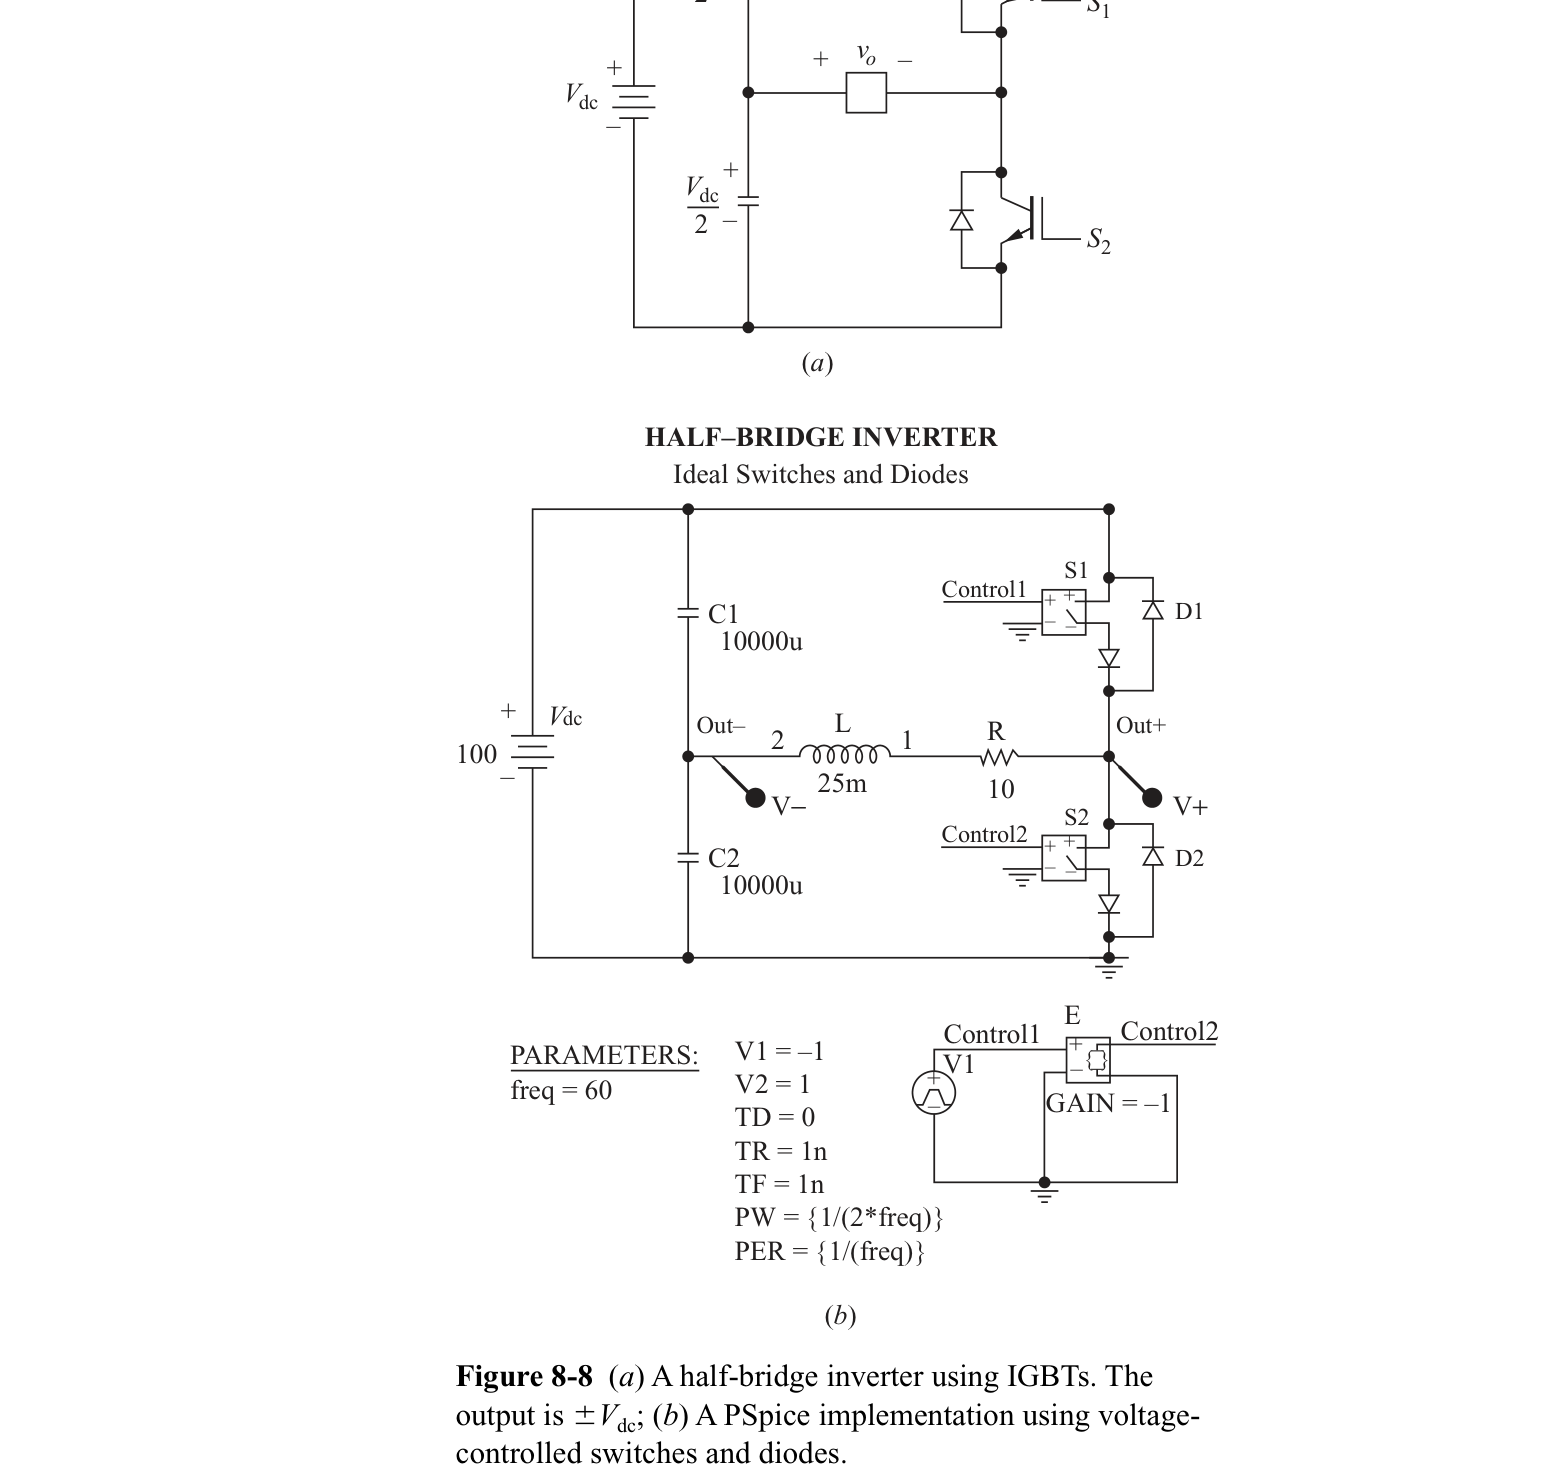
\includegraphics[width=0.68\textwidth]{hart_fig_8_1_half_bridge.png}
\caption{Single-phase half-bridge voltage source inverter: (a) Power circuit diagram with split DC source $V_{dc}/2$; (b) Square-wave output voltage $v_o(t)$ and inductive load current $i_o(t)$ waveforms showing conduction intervals of switches and freewheeling feedback diodes. (Source: Daniel W. Hart, Fig.\ 8-1)}
\label{fig:half_bridge}
\end{figure}

\begin{itemize}[leftmargin=*]
  \item \textbf{Interval 1 ($0 \le t < T/2$):} Switch $S_1$ is turned ON. Load terminal $A$ is connected to the positive DC rail ($+V_{dc}/2$ relative to center tap $O$):
  \begin{equation}
  v_o(t) = v_{AO}(t) = +\frac{V_{dc}}{2}
  \end{equation}
  \item \textbf{Interval 2 ($T/2 \le t < T$):} Switch $S_1$ is turned OFF, and $S_2$ is turned ON. Load terminal $A$ is connected to the negative DC rail ($-V_{dc}/2$):
  \begin{equation}
  v_o(t) = v_{AO}(t) = -\frac{V_{dc}}{2}
  \end{equation}
  \item \textbf{Freewheeling Diode Operation with Inductive Load:} If $S_1$ turns OFF while positive load current $i_o > 0$ is still flowing, inductor energy forces diode $D_2$ into conduction, clamping $v_o = -V_{dc}/2$ and feeding reactive energy back into the lower DC capacitor $C_2$ until $i_o$ decays to zero!
  \item \textbf{RMS Output Voltage:}
  \begin{equation}
  V_{or} = \sqrt{\frac{1}{T}\left[ \int_0^{T/2} \left(+\frac{V_{dc}}{2}\right)^2 dt + \int_{T/2}^T \left(-\frac{V_{dc}}{2}\right)^2 dt \right]} = \frac{V_{dc}}{2}
  \end{equation}
  \item \textbf{Major Limitations of the Half-Bridge Inverter:}
  \begin{enumerate}
    \item Requires a split three-wire DC supply or large center-tapped balancing capacitors.
    \item DC bus voltage utilization is low: the maximum peak-to-peak output voltage is only $V_{dc}$, yielding a fundamental peak of only $\hat{V}_{o1} = \frac{2}{\pi}V_{dc} \approx 0.637 V_{dc}$.
    \item Peak blocking voltage across the OFF-state switch equals the full DC supply $V_{dc} = 2 \times (V_{dc}/2)$, requiring devices rated for twice the output voltage!
  \end{enumerate}
\end{itemize}

\subsubsection{Single-Phase Full-Bridge (H-Bridge) Inverter Configuration}
The full-bridge inverter (Figure~\ref{fig:full_bridge}) eliminates the center-tap requirement by employing four controlled semiconductor switches ($S_1, S_2, S_3, S_4$) arranged in two phase legs ($A$ and $B$) across a single DC source $V_{dc}$.

\begin{figure}[htbp]
\centering
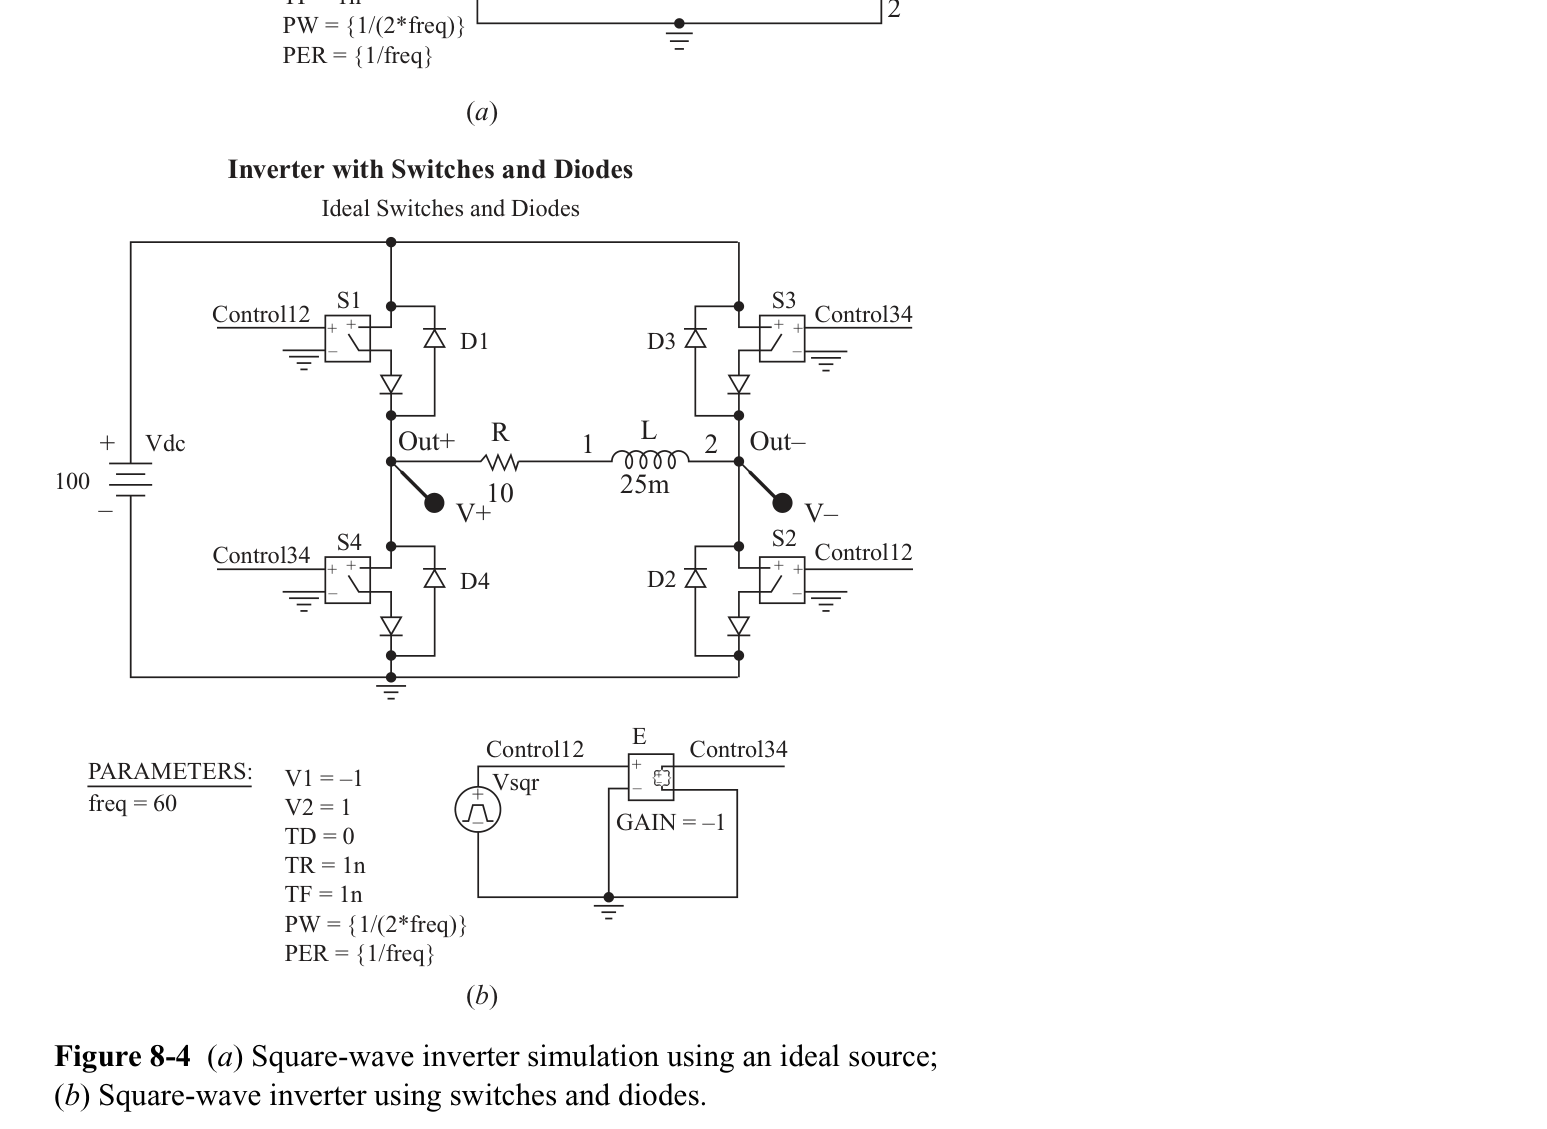
\includegraphics[width=0.68\textwidth]{hart_fig_8_4_full_bridge.png}
\caption{Single-phase full-bridge (H-bridge) inverter: (a) Power circuit diagram; (b) Square-wave output voltage $v_o(t) = v_A - v_B$ alternating between $+V_{dc}$ and $-V_{dc}$, and inductive load current $i_o(t)$. (Source: Daniel W. Hart, Fig.\ 8-4)}
\label{fig:full_bridge}
\end{figure}

\begin{itemize}[leftmargin=*]
  \item \textbf{Diagonal Pair Conduction:}
  \begin{itemize}
    \item When switches $(S_1, S_2)$ are gated ON: $v_{Ao} = +V_{dc}/2$ and $v_{Bo} = -V_{dc}/2$, producing output voltage:
    \begin{equation}
    v_o(t) = v_{AB}(t) = v_{Ao} - v_{Bo} = +V_{dc}
    \end{equation}
    \item When switches $(S_3, S_4)$ are gated ON: $v_{Ao} = -V_{dc}/2$ and $v_{Bo} = +V_{dc}/2$, producing output voltage:
    \begin{equation}
    v_o(t) = v_{AB}(t) = -V_{dc}
    \end{equation}
  \end{itemize}
  \item \textbf{RMS Output Voltage:}
  \begin{equation}
  V_{or} = \sqrt{\frac{1}{T}\int_0^T (\pm V_{dc})^2 dt} = V_{dc}
  \end{equation}
  The full-bridge produces \textbf{twice} the output voltage of the half-bridge for the same DC link voltage, yielding four times the output power into a given load resistance!
\end{itemize}

\subsection{Fourier Analysis and Harmonic Spectrum of Square-Wave Inverters}

The square-wave output voltage $v_o(t)$ of a full-bridge inverter alternating between $+V_{dc}$ and $-V_{dc}$ possesses \textbf{odd half-wave symmetry}:
\begin{equation}
v_o(\omega t) = -v_o(\omega t + \pi) \quad \text{and} \quad v_o(-\omega t) = -v_o(\omega t)
\end{equation}
Consequently, all DC offset and all even harmonics are identically zero ($a_0 = 0$, $a_n = 0$, $b_n = 0$ for even $n$). The Fourier series contains only odd sine harmonics:
\begin{equation}
b_n = \frac{2}{\pi} \int_0^\pi V_{dc} \sin(n\omega t) d(\omega t) = \frac{2V_{dc}}{n\pi} \left[-\cos(n\omega t)\right]_0^\pi = \frac{2V_{dc}}{n\pi} \left[1 - (-1)^n\right]
\end{equation}
For odd $n$ ($n = 1, 3, 5, 7, \dots$), $1 - (-1)^n = 2$:
\begin{formulabox}[Fourier Series of Single-Phase Full-Bridge Square-Wave Inverter]
\begin{equation}
v_o(t) = \sum_{n=1,3,5,\dots}^{\infty} \frac{4V_{dc}}{n\pi} \sin(n\omega t) = \frac{4V_{dc}}{\pi} \sin(\omega t) + \frac{4V_{dc}}{3\pi} \sin(3\omega t) + \frac{4V_{dc}}{5\pi} \sin(5\omega t) + \dots
\label{eq:fourier_square_full}
\end{equation}
\end{formulabox}

\subsubsection{Key Harmonic Metrics}
\begin{itemize}[leftmargin=*]
  \item \textbf{Peak Amplitude of Fundamental:} $\hat{V}_{o1} = \frac{4V_{dc}}{\pi} \approx 1.273 V_{dc}$.
  \item \textbf{RMS Value of Fundamental:} $V_{o1(rms)} = \frac{\hat{V}_{o1}}{\sqrt{2}} = \frac{4V_{dc}}{\sqrt{2}\pi} = \frac{2\sqrt{2}}{\pi}V_{dc} \approx 0.9003 V_{dc}$.
  \item \textbf{Harmonic Amplitudes:} The amplitude of the $n$-th harmonic decreases inversely with harmonic order:
  \begin{equation}
  \hat{V}_{on} = \frac{\hat{V}_{o1}}{n} \implies \frac{V_{on}}{V_{o1}} = \frac{1}{n}
  \end{equation}
  Specifically: 3rd harmonic is $33.3\%$ of fundamental, 5th harmonic is $20\%$, 7th harmonic is $14.3\%$.
  \item \textbf{Total Harmonic Distortion (THD) of Voltage:}
  \begin{equation}
  \text{THD}_v = \frac{\sqrt{V_{or}^2 - V_{o1(rms)}^2}}{V_{o1(rms)}} = \frac{\sqrt{V_{dc}^2 - \left(\frac{2\sqrt{2}}{\pi}V_{dc}\right)^2}}{\frac{2\sqrt{2}}{\pi}V_{dc}} = \sqrt{\frac{\pi^2}{8} - 1} \approx \sqrt{1.2337 - 1} = 0.4834 \implies 48.34\%
  \end{equation}
  A total harmonic distortion of $48.34\%$ is severe and unacceptable for sensitive AC loads or utility grid interconnection, motivating the necessity of Pulse Width Modulation (PWM)!
\end{itemize}

\subsection{Sinusoidal Pulse Width Modulation (SPWM)}

In \textbf{Sinusoidal Pulse Width Modulation (SPWM)}, the inverter switches are turned ON and OFF multiple times per half-cycle at a high switching frequency. The widths of the gating pulses are modulated proportionally to the instantaneous amplitude of a sinusoidal reference wave.

\subsubsection{Fundamental Definitions and Modulation Parameters}
\begin{enumerate}[leftmargin=*]
  \item \textbf{Modulating / Reference Wave ($v_{\text{control}}$ or $v_{\text{sine}}$):} A low-frequency sinusoidal voltage whose frequency $f_o$ defines the fundamental output frequency of the inverter, and whose peak amplitude $\hat{V}_{\text{control}}$ dictates the output voltage magnitude.
  \item \textbf{Carrier Wave ($v_{\text{tri}}$):} A high-frequency symmetrical triangular waveform of frequency $f_s$ (or $f_c$) and peak amplitude $\hat{V}_{\text{tri}}$.
  \item \textbf{Amplitude Modulation Index ($m_a$):}
  \begin{formulabox}[Amplitude Modulation Index]
  \begin{equation}
  m_a = \frac{\hat{V}_{\text{control}}}{\hat{V}_{\text{tri}}}
  \label{eq:ma_def}
  \end{equation}
  \end{formulabox}
  $m_a$ governs the amplitude of the fundamental output voltage component.
  \item \textbf{Frequency Modulation Ratio ($m_f$):}
  \begin{formulabox}[Frequency Modulation Ratio]
  \begin{equation}
  m_f = \frac{f_s}{f_o} = \frac{f_{\text{carrier}}}{f_{\text{reference}}}
  \label{eq:mf_def}
  \end{equation}
  \end{formulabox}
  $m_f$ determines the frequency at which switching harmonics appear in the output spectrum.
\end{enumerate}

\subsection{PWM with Bipolar Voltage Switching}

In bipolar voltage switching, the diagonally opposite switch pairs $(S_1, S_2)$ and $(S_3, S_4)$ in the full bridge are switched simultaneously in complementary fashion:
\begin{itemize}[leftmargin=*]
  \item When $v_{\text{control}} > v_{\text{tri}}$: Switches $S_1$ and $S_2$ are ON $\implies v_o(t) = +V_{dc}$.
  \item When $v_{\text{control}} < v_{\text{tri}}$: Switches $S_3$ and $S_4$ are ON $\implies v_o(t) = -V_{dc}$.
\end{itemize}
Because the output voltage transitions directly between the two extreme polarities ($+V_{dc}$ and $-V_{dc}$), this scheme is termed \textbf{bipolar switching}.

\begin{figure}[htbp]
\centering
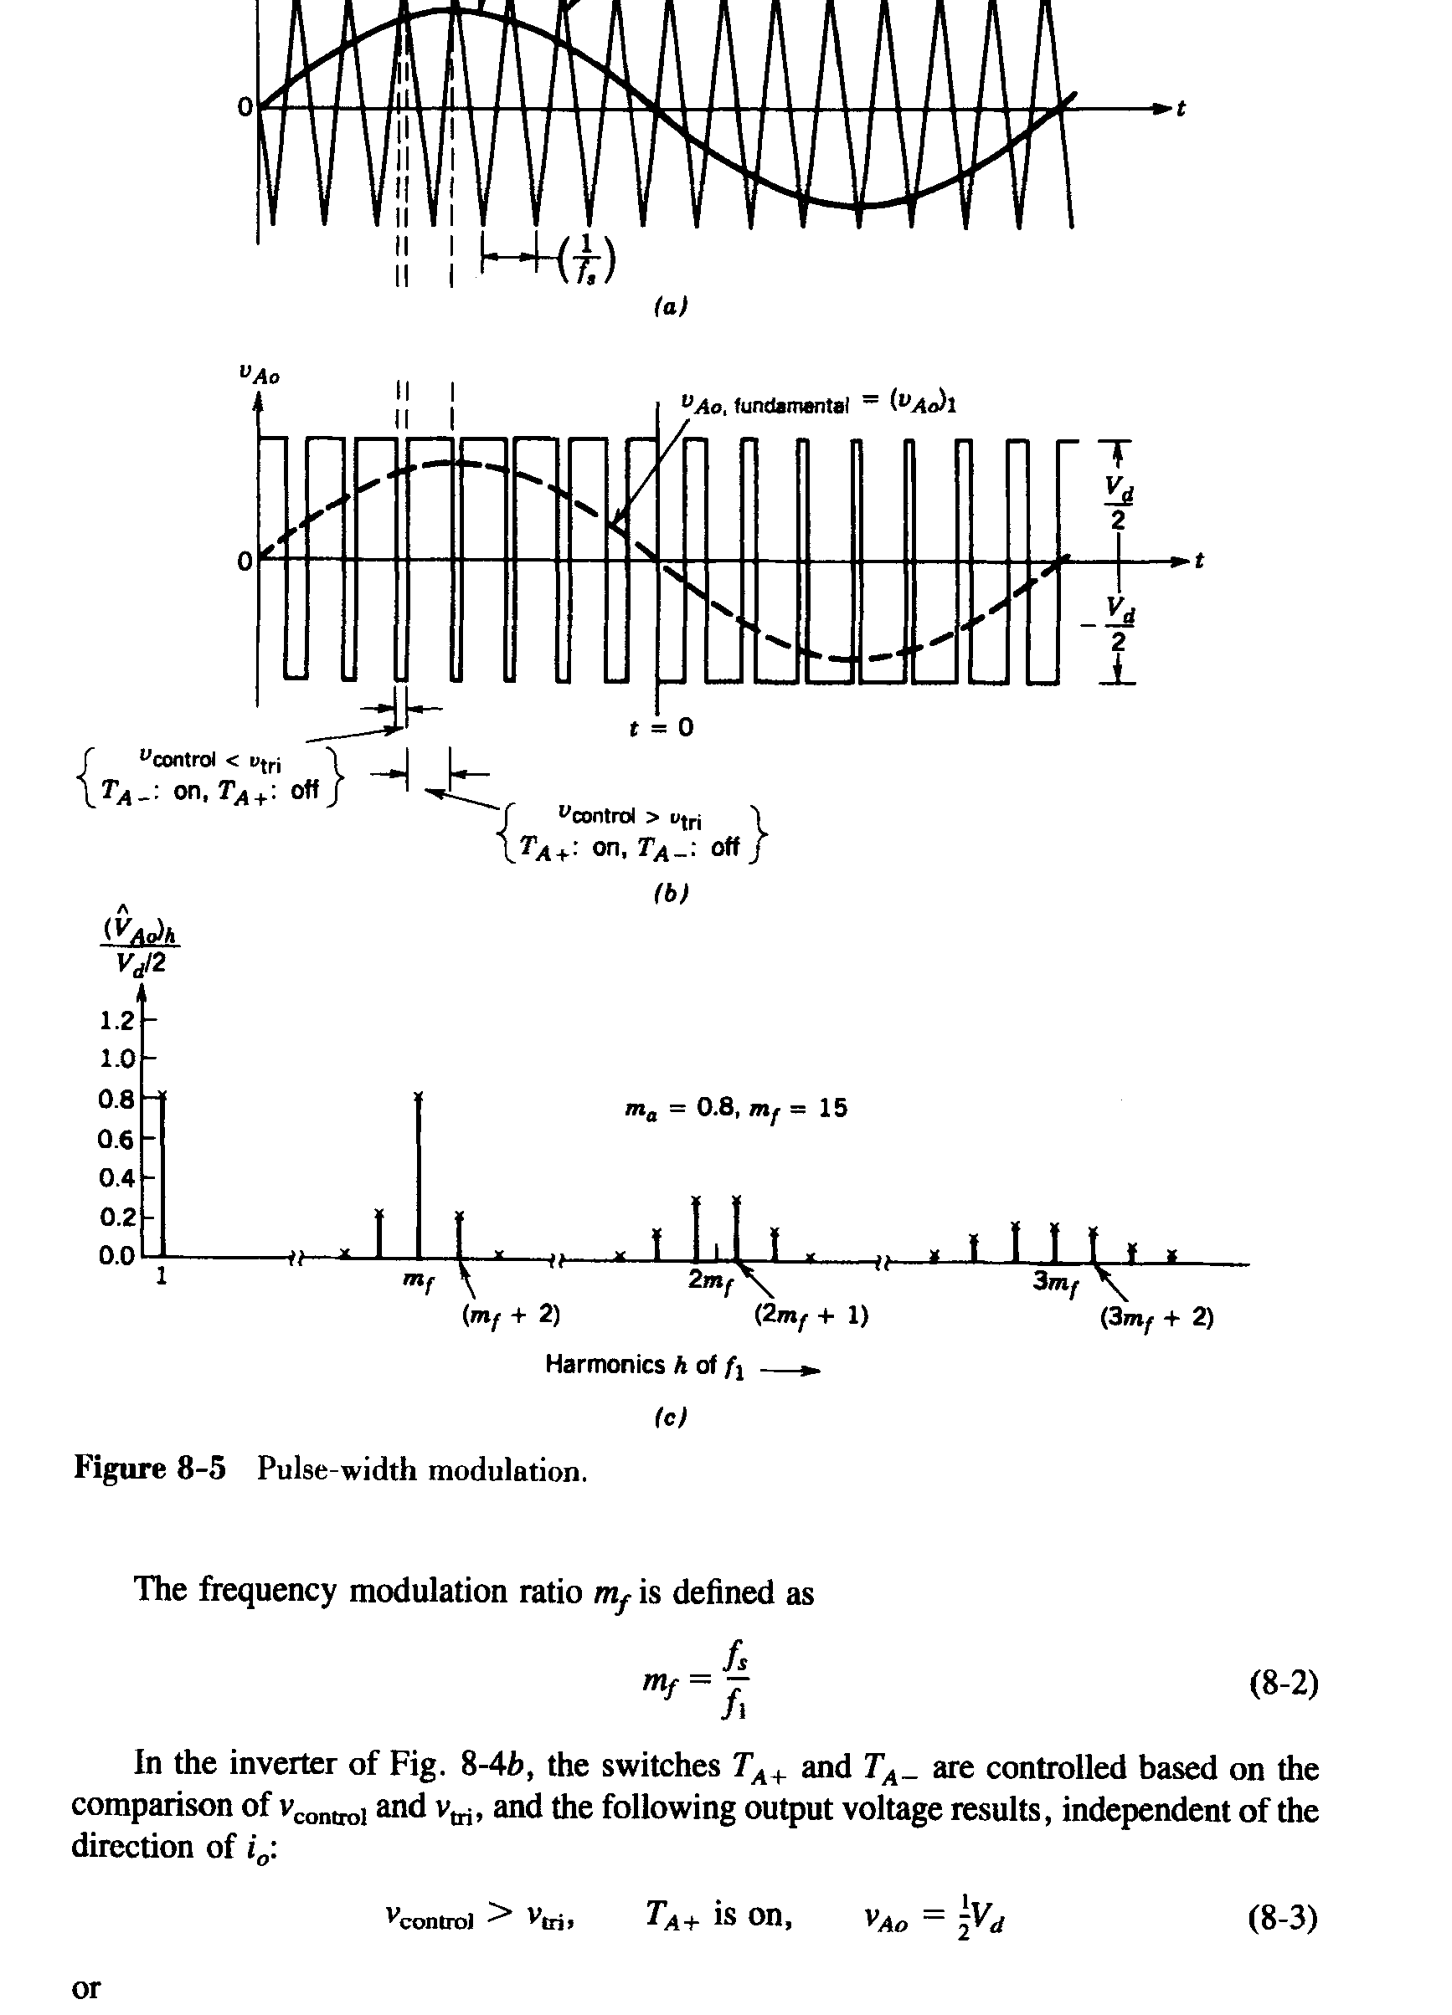
\includegraphics[width=0.72\textwidth]{mohan_fig_8_5_bipolar_pwm.png}
\caption{Pulse-width modulation with bipolar voltage switching: (a) Comparison of sinusoidal reference $v_{\text{control}}$ and triangular carrier $v_{\text{tri}}$; (b) Switched pole voltages $v_{Ao}$ and $v_{Bo}$; (c) Bipolar output voltage $v_o(t)$ alternating between $+V_{dc}$ and $-V_{dc}$; (d) Harmonic spectrum showing fundamental at $f_1$ and harmonic sidebands centered around $m_f, 2m_f, 3m_f$. (Source: Ned Mohan, Fig.\ 8-5)}
\label{fig:bipolar_pwm}
\end{figure}

\subsubsection{Harmonic Characteristics of Bipolar PWM}
\begin{itemize}[leftmargin=*]
  \item \textbf{Fundamental Peak Voltage in Linear Range ($m_a \le 1.0$):}
  \begin{equation}
  \hat{V}_{o1} = m_a V_{dc} \implies V_{o1(rms)} = \frac{m_a V_{dc}}{\sqrt{2}} \approx 0.707 m_a V_{dc}
  \end{equation}
  The fundamental output voltage is strictly linearly proportional to the modulation index $m_a$.
  \item \textbf{Harmonic Sidebands:} Harmonics appear as sidebands clustered around the switching frequency and its integer multiples:
  \begin{equation}
  f_h = \left(j \cdot m_f \pm k\right) f_o
  \end{equation}
  where the harmonic order $h = j \cdot m_f \pm k$.
  \item \textbf{Selection Rules for $m_f$:}
  \begin{itemize}
    \item $m_f$ should be chosen as an \textbf{odd integer}. This establishes \textbf{odd half-wave symmetry} ($v_o(\omega t + \pi) = -v_o(\omega t)$), which completely eliminates all even harmonics from the output spectrum!
    \item If $m_f$ is an odd integer, the dominant harmonics occur at $m_f$ and $m_f \pm 2$.
    \item Synchronous PWM ($m_f = \text{integer}$) is essential for $m_f < 21$ to prevent sub-harmonic frequencies. For $m_f > 21$, asynchronous PWM can be utilized.
  \end{itemize}
\end{itemize}

\subsection{PWM with Unipolar Voltage Switching}

In unipolar voltage switching, the two inverter legs are controlled independently by comparing the carrier wave $v_{\text{tri}}$ with two reference sine waves that are $180^\circ$ out of phase:
\begin{itemize}[leftmargin=*]
  \item \textbf{Leg A Control:} $v_{\text{control}}$ is compared with $v_{\text{tri}}$:
  \begin{itemize}
    \item If $v_{\text{control}} > v_{\text{tri}}$: Switch $S_1$ is ON ($v_{Ao} = +V_{dc}/2$).
    \item If $v_{\text{control}} < v_{\text{tri}}$: Switch $S_4$ is ON ($v_{Ao} = -V_{dc}/2$).
  \end{itemize}
  \item \textbf{Leg B Control:} $-v_{\text{control}}$ is compared with $v_{\text{tri}}$:
  \begin{itemize}
    \item If $-v_{\text{control}} > v_{\text{tri}}$: Switch $S_3$ is ON ($v_{Bo} = +V_{dc}/2$).
    \item If $-v_{\text{control}} < v_{\text{tri}}$: Switch $S_2$ is ON ($v_{Bo} = -V_{dc}/2$).
  \end{itemize}
\end{itemize}

\begin{figure}[htbp]
\centering
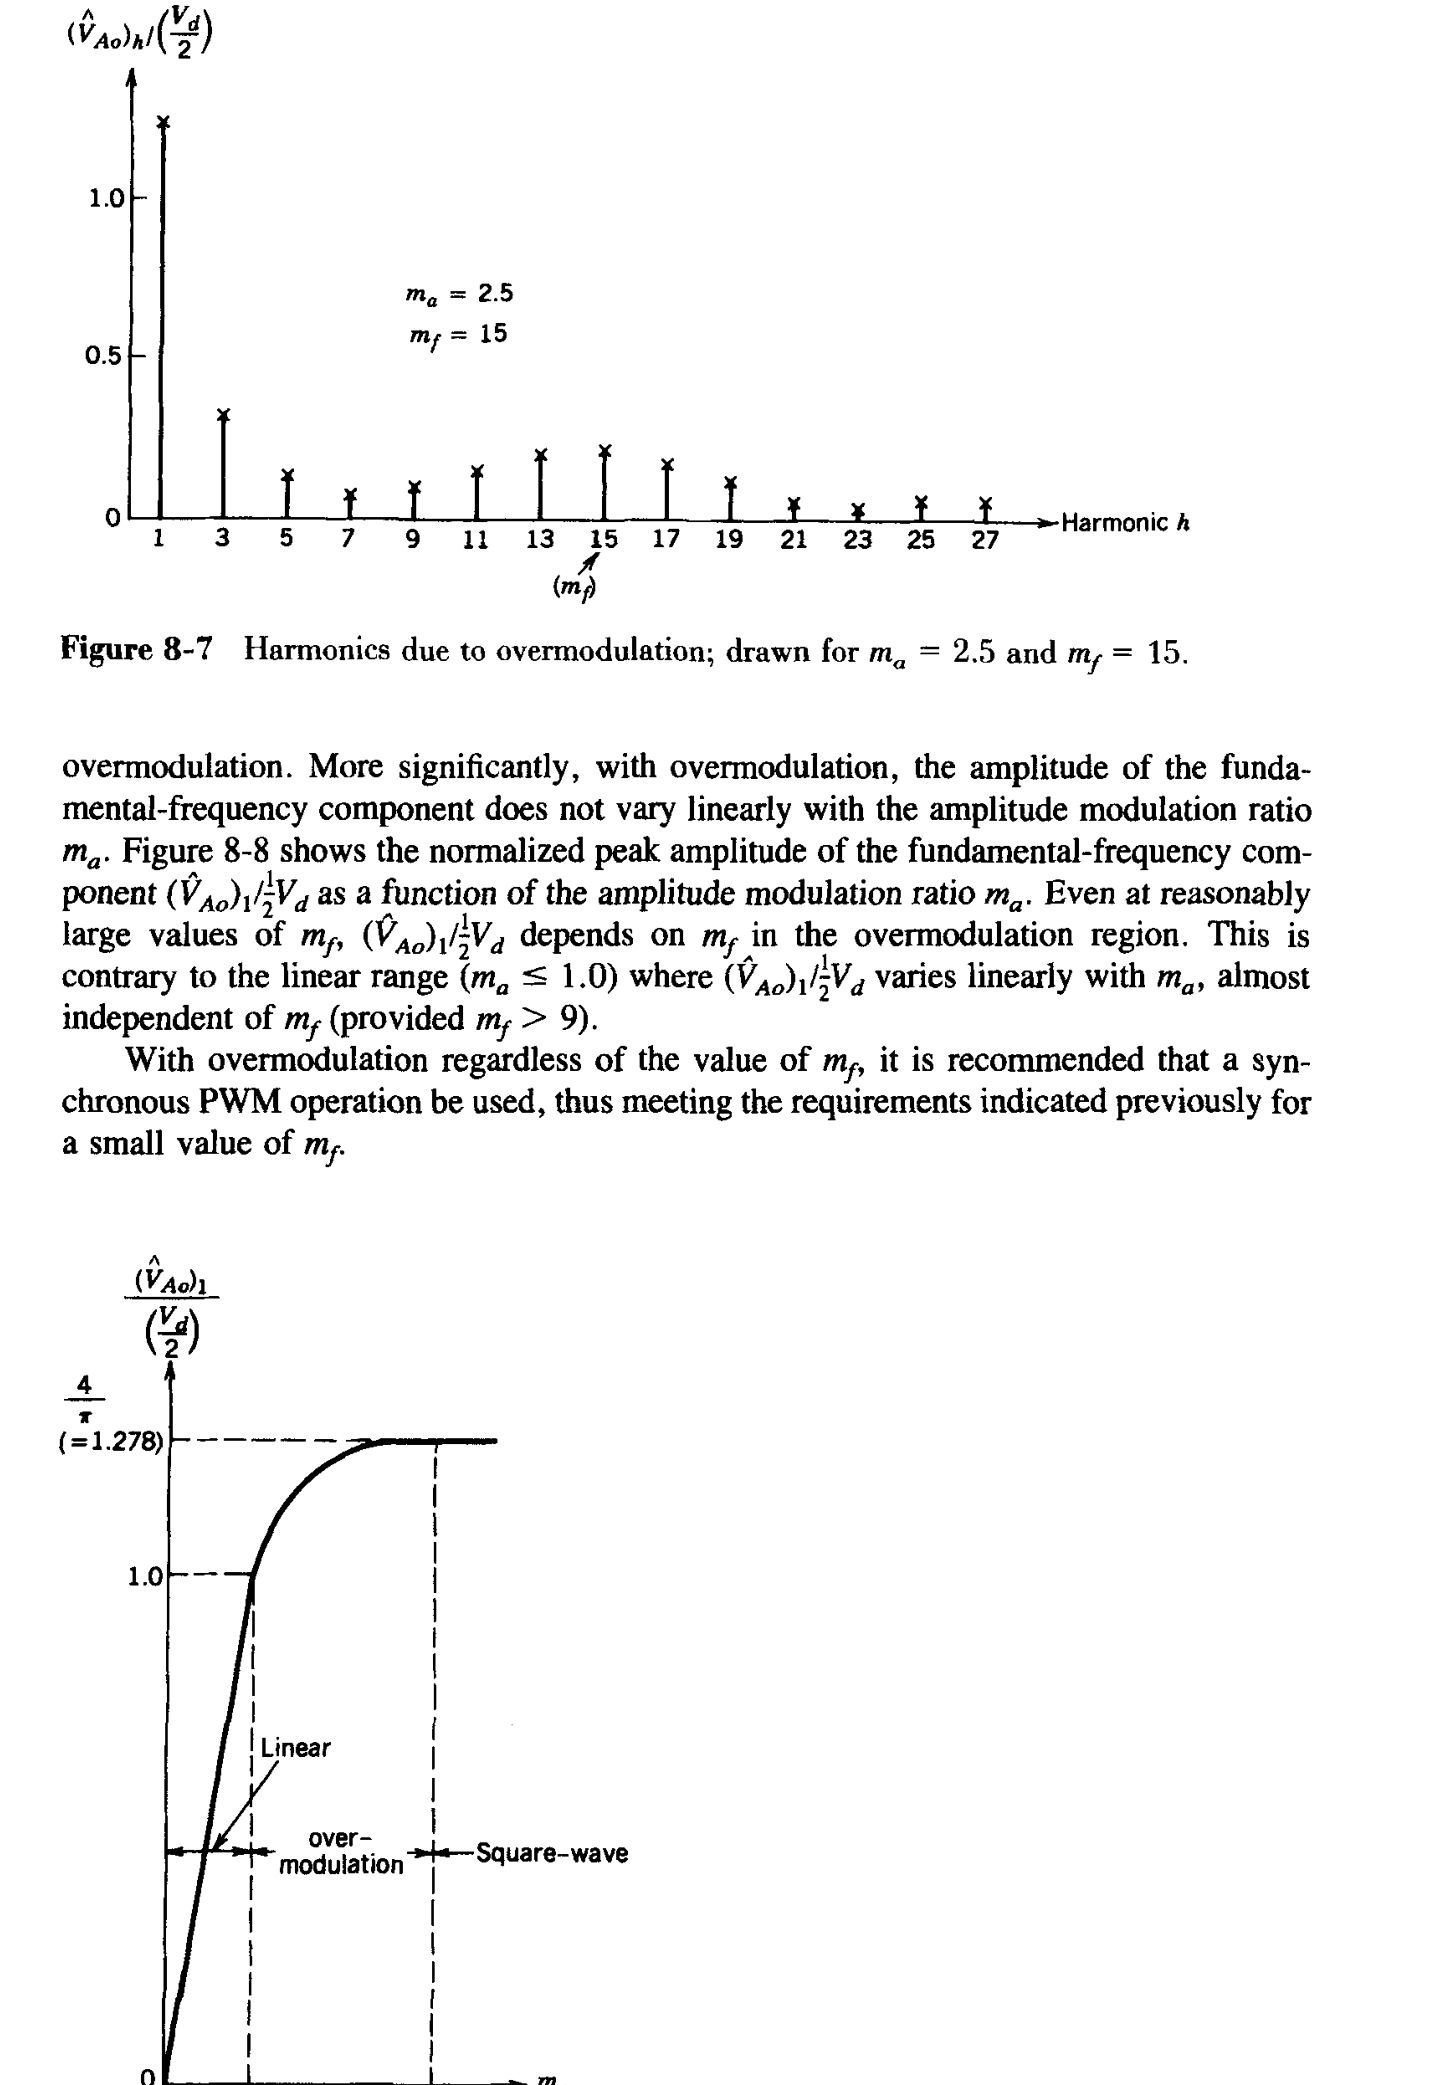
\includegraphics[width=0.72\textwidth]{mohan_fig_8_11_unipolar_pwm.png}
\caption{Pulse-width modulation with unipolar voltage switching: (a) Reference waves $v_{\text{control}}$ and $-v_{\text{control}}$ compared with carrier $v_{\text{tri}}$; (b) Pole voltages $v_{Ao}$ and $v_{Bo}$; (c) Unipolar output voltage $v_o(t)$ switching between $0$ and $+V_{dc}$ or $0$ and $-V_{dc}$; (d) Harmonic spectrum showing the total absence of harmonics around $m_f$ and first harmonic cluster shifted to $2m_f$. (Source: Ned Mohan, Fig.\ 8-11)}
\label{fig:unipolar_pwm}
\end{figure}

\subsubsection{The Remarkable Advantages of Unipolar PWM}
During each switching event, the output voltage transitions between \textbf{three voltage levels}: $+V_{dc}$, $0$, and $-V_{dc}$:
\begin{itemize}
  \item During the positive half-cycle of $v_{\text{control}}$, $v_o(t)$ switches between $0$ and $+V_{dc}$.
  \item During the negative half-cycle of $v_{\text{control}}$, $v_o(t)$ switches between $0$ and $-V_{dc}$.
\end{itemize}
\begin{conceptbox}[Why Unipolar Switching Outperforms Bipolar Switching]
\begin{enumerate}
  \item \textbf{Doubling of Effective Switching Frequency:} The output voltage pulses appear at \textbf{twice the carrier frequency} ($2f_s$). The fundamental output voltage equation remains identical:
  \begin{equation}
  \hat{V}_{o1} = m_a V_{dc} \quad (0 \le m_a \le 1.0)
  \end{equation}
  \item \textbf{Cancellation of Harmonics at $m_f$:} Harmonics centered around $m_f, 3m_f, 5m_f, \dots$ are completely cancelled out! The lowest-order harmonic sidebands appear centered around $2m_f$:
  \begin{equation}
  h = 2m_f \pm 1, \quad 2m_f \pm 3
  \end{equation}
  \item \textbf{Dramatically Smaller Output Filter:} Because the lowest harmonic frequency is doubled ($2f_s$), the required inductance and capacitance of the output low-pass filter are cut in half, slashing converter weight, volume, and cost!
  \item \textbf{Reduced Current Ripple:} Load current ripple is substantially smaller compared to bipolar PWM for identical device switching frequencies.
\end{enumerate}
\end{conceptbox}

\begin{table}[htbp]
\centering
\small
\caption{Comprehensive Comparison: Bipolar vs. Unipolar PWM Schemes}
\label{tab:bipolar_vs_unipolar}
\begin{tabularx}{\textwidth}{l X X}
\toprule
\textbf{Feature} & \textbf{Bipolar PWM} & \textbf{Unipolar PWM} \\
\midrule
\textbf{Output Voltage Levels} & 2 levels: $+V_{dc}, -V_{dc}$ & 3 levels: $+V_{dc}, 0, -V_{dc}$ \\
\textbf{Leg Control} & Legs A and B switched simultaneously & Legs A and B switched independently \\
\textbf{Carrier References} & Single sine wave $v_{\text{control}}$ & Complementary pair: $+v_{\text{control}}, -v_{\text{control}}$ \\
\textbf{Selection of $m_f$} & $m_f$ must be an odd integer & $m_f$ is typically chosen as an even integer \\
\textbf{Effective Output Frequency} & $f_s$ (Carrier frequency) & $2f_s$ (Double carrier frequency) \\
\textbf{Dominant Harmonics} & Clustered around $m_f, 2m_f, 3m_f$ & Absent at $m_f$; first appear around $2m_f$ \\
\textbf{Output Filter Size} & Large & Significantly smaller ($\approx 50\%$ reduction) \\
\textbf{Switching Stress ($dv/dt$)} & Steps of $2V_{dc}$ across load terminals & Steps of $V_{dc}$ across load terminals \\
\textbf{Control Complexity} & Minimal & Moderately higher \\
\bottomrule
\end{tabularx}
\end{table}

\subsection{Operating Modes: Linear Modulation, Overmodulation, and Square-Wave}

The relationship between the fundamental output voltage $\hat{V}_{o1}$ and the modulation index $m_a$ spans three distinct operational regimes:

\begin{enumerate}[leftmargin=*]
  \item \textbf{Linear Modulation Region ($0 \le m_a \le 1.0$):}
  \begin{itemize}
    \item The peak of the modulating sine wave is less than or equal to the triangular carrier peak ($\hat{V}_{\text{control}} \le \hat{V}_{\text{tri}}$).
    \item The fundamental peak output voltage varies strictly linearly with $m_a$:
    \begin{equation}
    \hat{V}_{o1} = m_a V_{dc}
    \end{equation}
    \item The harmonic frequencies are independent of $m_a$, and harmonic amplitudes are directly proportional to $m_a$.
  \end{itemize}

  \item \textbf{Overmodulation Region ($1.0 < m_a \le 3.24$):}
  \begin{itemize}
    \item The reference sine wave amplitude exceeds the carrier peak ($\hat{V}_{\text{control}} > \hat{V}_{\text{tri}}$).
    \item For intervals near the sine wave peaks, the reference wave completely exceeds the triangular carrier, resulting in \textbf{pulse dropping}—the switch remains continuously ON for multiple carrier cycles without pulsing.
    \item The relationship between $\hat{V}_{o1}$ and $m_a$ becomes \textbf{non-linear} and begins to saturate.
    \item Low-order harmonics (3rd, 5th, 7th) re-appear directly in the output voltage spectrum, increasing harmonic distortion. However, overmodulation is widely utilized in industrial AC motor drives to extract maximum fundamental voltage during high-speed operation!
  \end{itemize}

  \item \textbf{Square-Wave Operation ($m_a > 3.24$):}
  \begin{itemize}
    \item As $m_a$ becomes large ($m_a > 3.24$), the PWM pulses merge completely into a single square wave per half-cycle.
    \item The inverter operates in pure square-wave mode, and the fundamental peak saturates at its absolute theoretical maximum:
    \begin{equation}
    \hat{V}_{o1,\text{max}} = \frac{4V_{dc}}{\pi} \approx 1.273 V_{dc}
    \end{equation}
    \item In this regime, the output voltage is completely independent of $m_a$ and can only be regulated by varying the input DC link voltage $V_{dc}$.
  \end{itemize}
\end{enumerate}

\subsection{The Critical Need for Blanking Time (Dead-Time)}

In practical bridge inverters, power semiconductor switches (IGBTs, MOSFETs) do not turn OFF instantaneously due to stored minority carrier recombination and gate charge discharging times ($t_{off} > t_{on}$).

\begin{figure}[htbp]
\centering
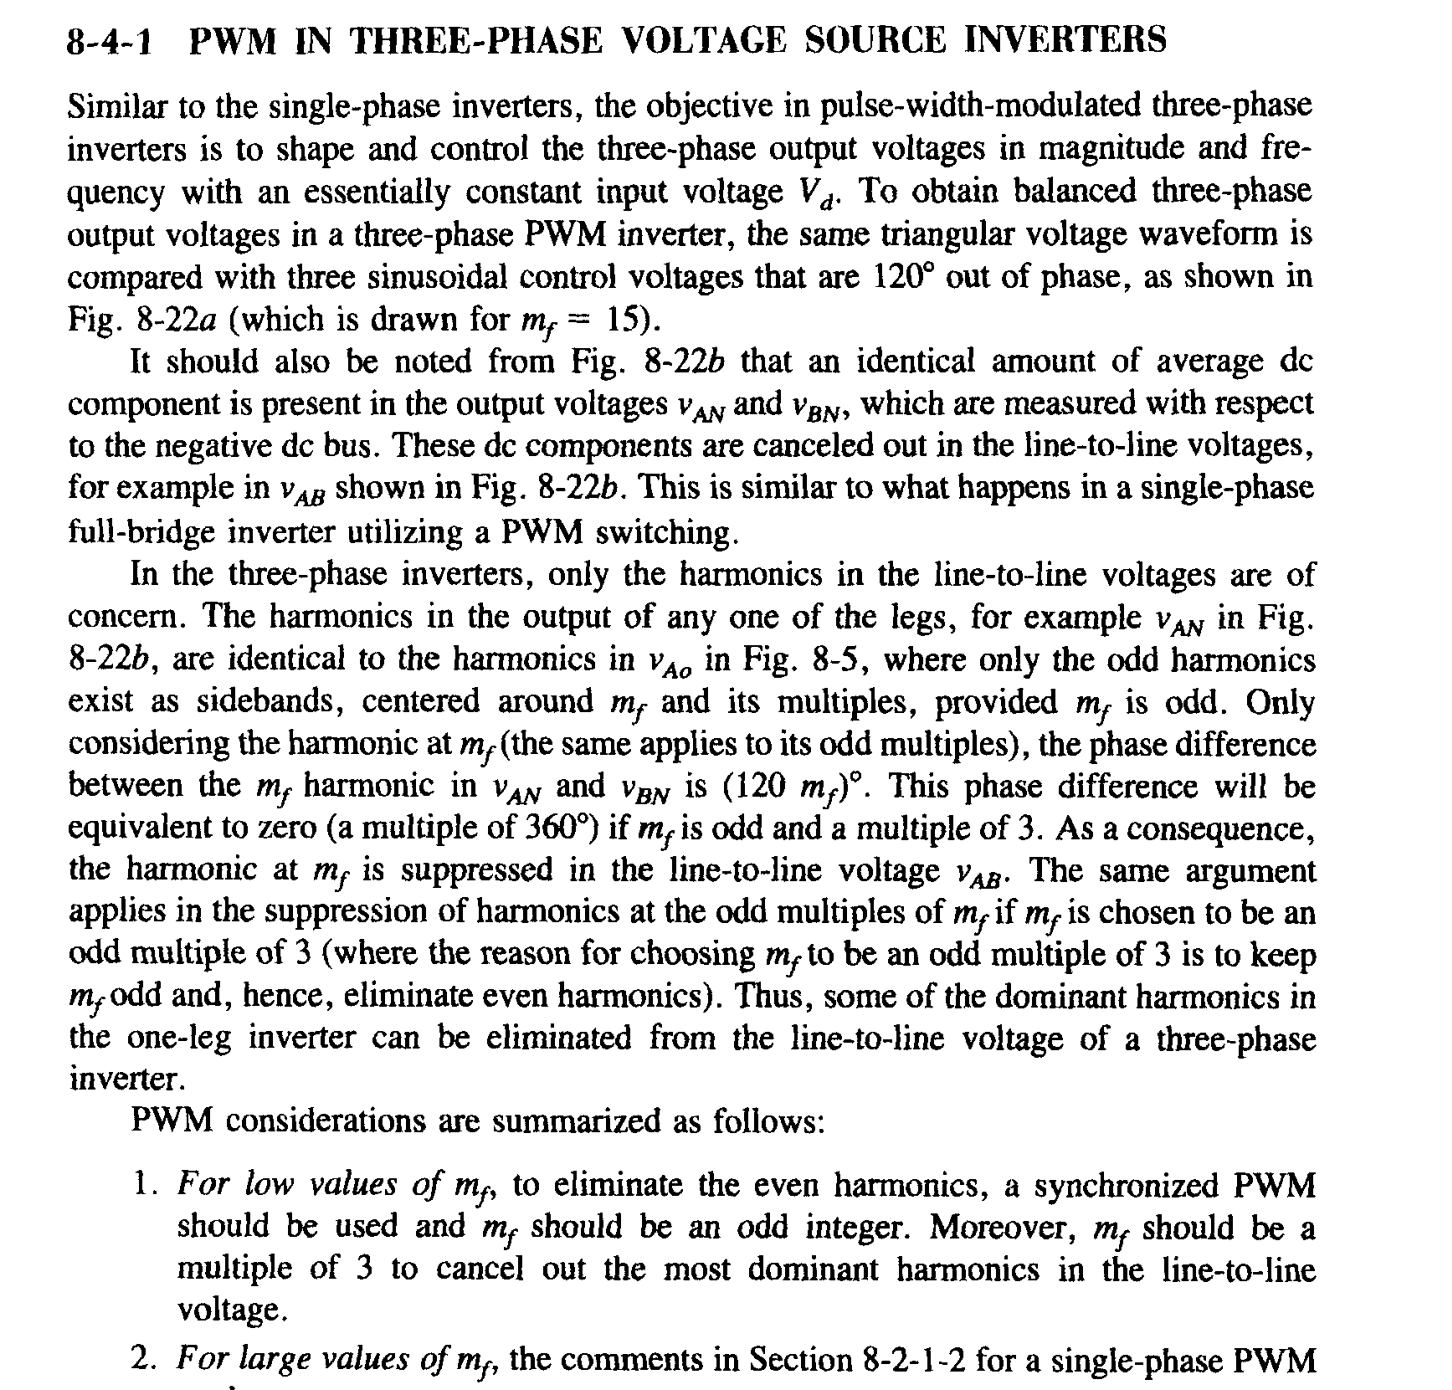
\includegraphics[width=0.72\textwidth]{mohan_fig_8_31_blanking_time.png}
\caption{Effect of blanking time (dead time) in a bridge inverter: (a) Inverter leg showing upper and lower switches and freewheeling diodes; (b) Gate signals with blanking time $t_\Delta$; (c) Resulting pole voltage waveforms showing voltage reduction for positive current and voltage increase for negative current. (Source: Ned Mohan, Fig.\ 8-31)}
\label{fig:blanking_time}
\end{figure}

\subsubsection{The Shoot-Through Catastrophe}
If the turn-ON gate command is applied to the upper switch ($S_1$) at the exact instant the turn-OFF command is sent to the lower switch ($S_4$) in the same leg, both switches will be simultaneously ON for the turn-off duration $t_{off}$. This creates a zero-impedance \textbf{shoot-through dead short circuit directly across the DC bus}:
\begin{equation}
I_{\text{fault}} = \frac{V_{dc}}{R_{\text{parasitic}}} \to \text{Thousands of Amperes} \implies \text{Explosive device destruction!}
\end{equation}

\subsubsection{Implementation of Blanking Time ($t_d$ or $t_\Delta$)}
To prevent shoot-through, a deliberate hardware/software delay called \textbf{blanking time} (or \textbf{dead-time}, $t_d$) is inserted between the turn-OFF command of one switch and the turn-ON command of the complementary switch in the same leg:
\begin{equation}
t_d > t_{off,\text{max}} + t_{\text{driver delay mismatch}}
\end{equation}
Typical values: $1.0 - 3.0\,\mu\text{s}$ for IGBTs; $100 - 500\text{ ns}$ for silicon MOSFETs; $< 50\text{ ns}$ for GaN HEMTs.

\subsubsection{Adverse Effects and Voltage Penalty Caused by Blanking Time}
During the blanking interval $t_d$, both controlled switches in the leg are commanded OFF. The actual pole voltage is determined entirely by the \textbf{direction of the load current} flowing through the freewheeling diodes:
\begin{itemize}[leftmargin=*]
  \item \textbf{When $i_o > 0$:} The current must flow through lower diode $D_4$. Even though $S_1$ was commanded ON, the pole voltage is clamped to $0\text{ V}$ instead of $+V_{dc}$. The pulse width is reduced by $t_d$, causing a loss of output voltage!
  \item \textbf{When $i_o < 0$:} The current flows through upper diode $D_1$, clamping the pole voltage to $+V_{dc}$ instead of $0\text{ V}$. The pulse width is increased by $t_d$.
  \item \textbf{Fundamental Voltage Drop:} Averaging this error over one fundamental cycle results in an average fundamental voltage reduction of:
  \begin{equation}
  \Delta V_o = \frac{4 t_d}{T_s} V_{dc} = 4 f_s t_d V_{dc}
  \label{eq:deadtime_voltage_drop}
  \end{equation}
  \item \textbf{Adverse Consequences:}
  \begin{enumerate}
    \item Causes a noticeable reduction in fundamental output voltage, especially prominent at low modulation indices.
    \item Generates severe \textbf{low-order harmonics} (5th, 7th, 11th) that are in-phase with current zero-crossings, producing torque pulsations in AC motors.
    \item Introduces waveform distortion and zero-crossing deadbands in precision motor drives.
  \end{enumerate}
\end{itemize}


\section{Three-Phase Pulse Width Modulated Voltage Source Inverters}

\subsection{Three-Phase Bridge Inverter Topology and Conduction Mechanics}

The three-phase voltage source inverter (Figure~\ref{fig:3ph_inverter_ckt}) is the universal industry-standard power conversion topology for variable-frequency AC motor drives (VFDs), grid-tied solar photovoltaic central inverters, wind turbine grid converters, and electric vehicle traction drives ($50\text{ kW} - 300\text{ kW}$).

The topology comprises six controlled switches ($S_1$ through $S_6$) arranged in three inverter legs ($A, B, C$) across a common DC link voltage $V_{dc}$, with six anti-parallel freewheeling diodes ($D_1$ through $D_6$).

\begin{figure}[htbp]
\centering
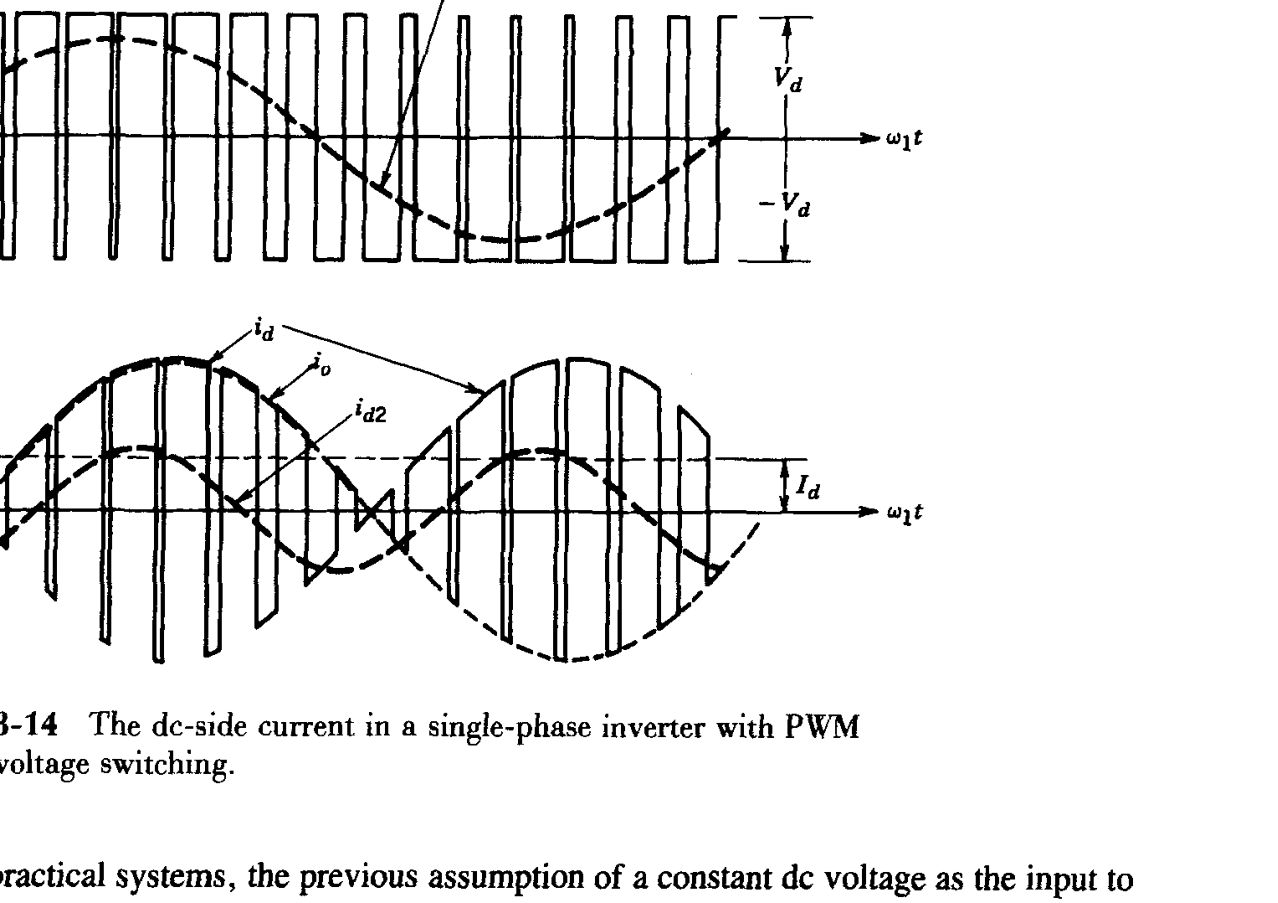
\includegraphics[width=0.75\textwidth]{mohan_fig_8_21_3ph_inverter_ckt.png}
\caption{Three-phase switch-mode voltage source inverter power circuit: Three phase legs ($A, B, C$) feeding a three-phase star ($Y$) or delta ($\Delta$) connected AC load from a stiff DC link capacitor bank. (Source: Ned Mohan, Fig.\ 8-21)}
\label{fig:3ph_inverter_ckt}
\end{figure}

\subsubsection{Switch Numbering and Firing Sequence}
The switches are traditionally numbered according to their natural firing sequence in a balanced three-phase cycle:
\begin{itemize}[leftmargin=*]
  \item Upper switches: $S_1$ (Phase A), $S_3$ (Phase B), $S_5$ (Phase C).
  \item Lower switches: $S_4$ (Phase A), $S_6$ (Phase B), $S_2$ (Phase C).
  \item Firing sequence: $S_1 \to S_2 \to S_3 \to S_4 \to S_5 \to S_6$, spaced by intervals of $60^\circ$ ($\pi/3$).
\end{itemize}

\subsection{Sinusoidal PWM in Three-Phase VSIs}

In three-phase SPWM, three balanced sinusoidal reference voltages displaced by $120^\circ$ are compared against a common high-frequency triangular carrier wave $v_{\text{tri}}$:
\begin{align}
v_{\text{control},A} &= \hat{V}_{\text{control}} \sin(\omega t) \notag\\
v_{\text{control},B} &= \hat{V}_{\text{control}} \sin(\omega t - 120^\circ) \notag\\
v_{\text{control},C} &= \hat{V}_{\text{control}} \sin(\omega t - 240^\circ) = \hat{V}_{\text{control}} \sin(\omega t + 120^\circ)
\end{align}

\begin{figure}[htbp]
\centering
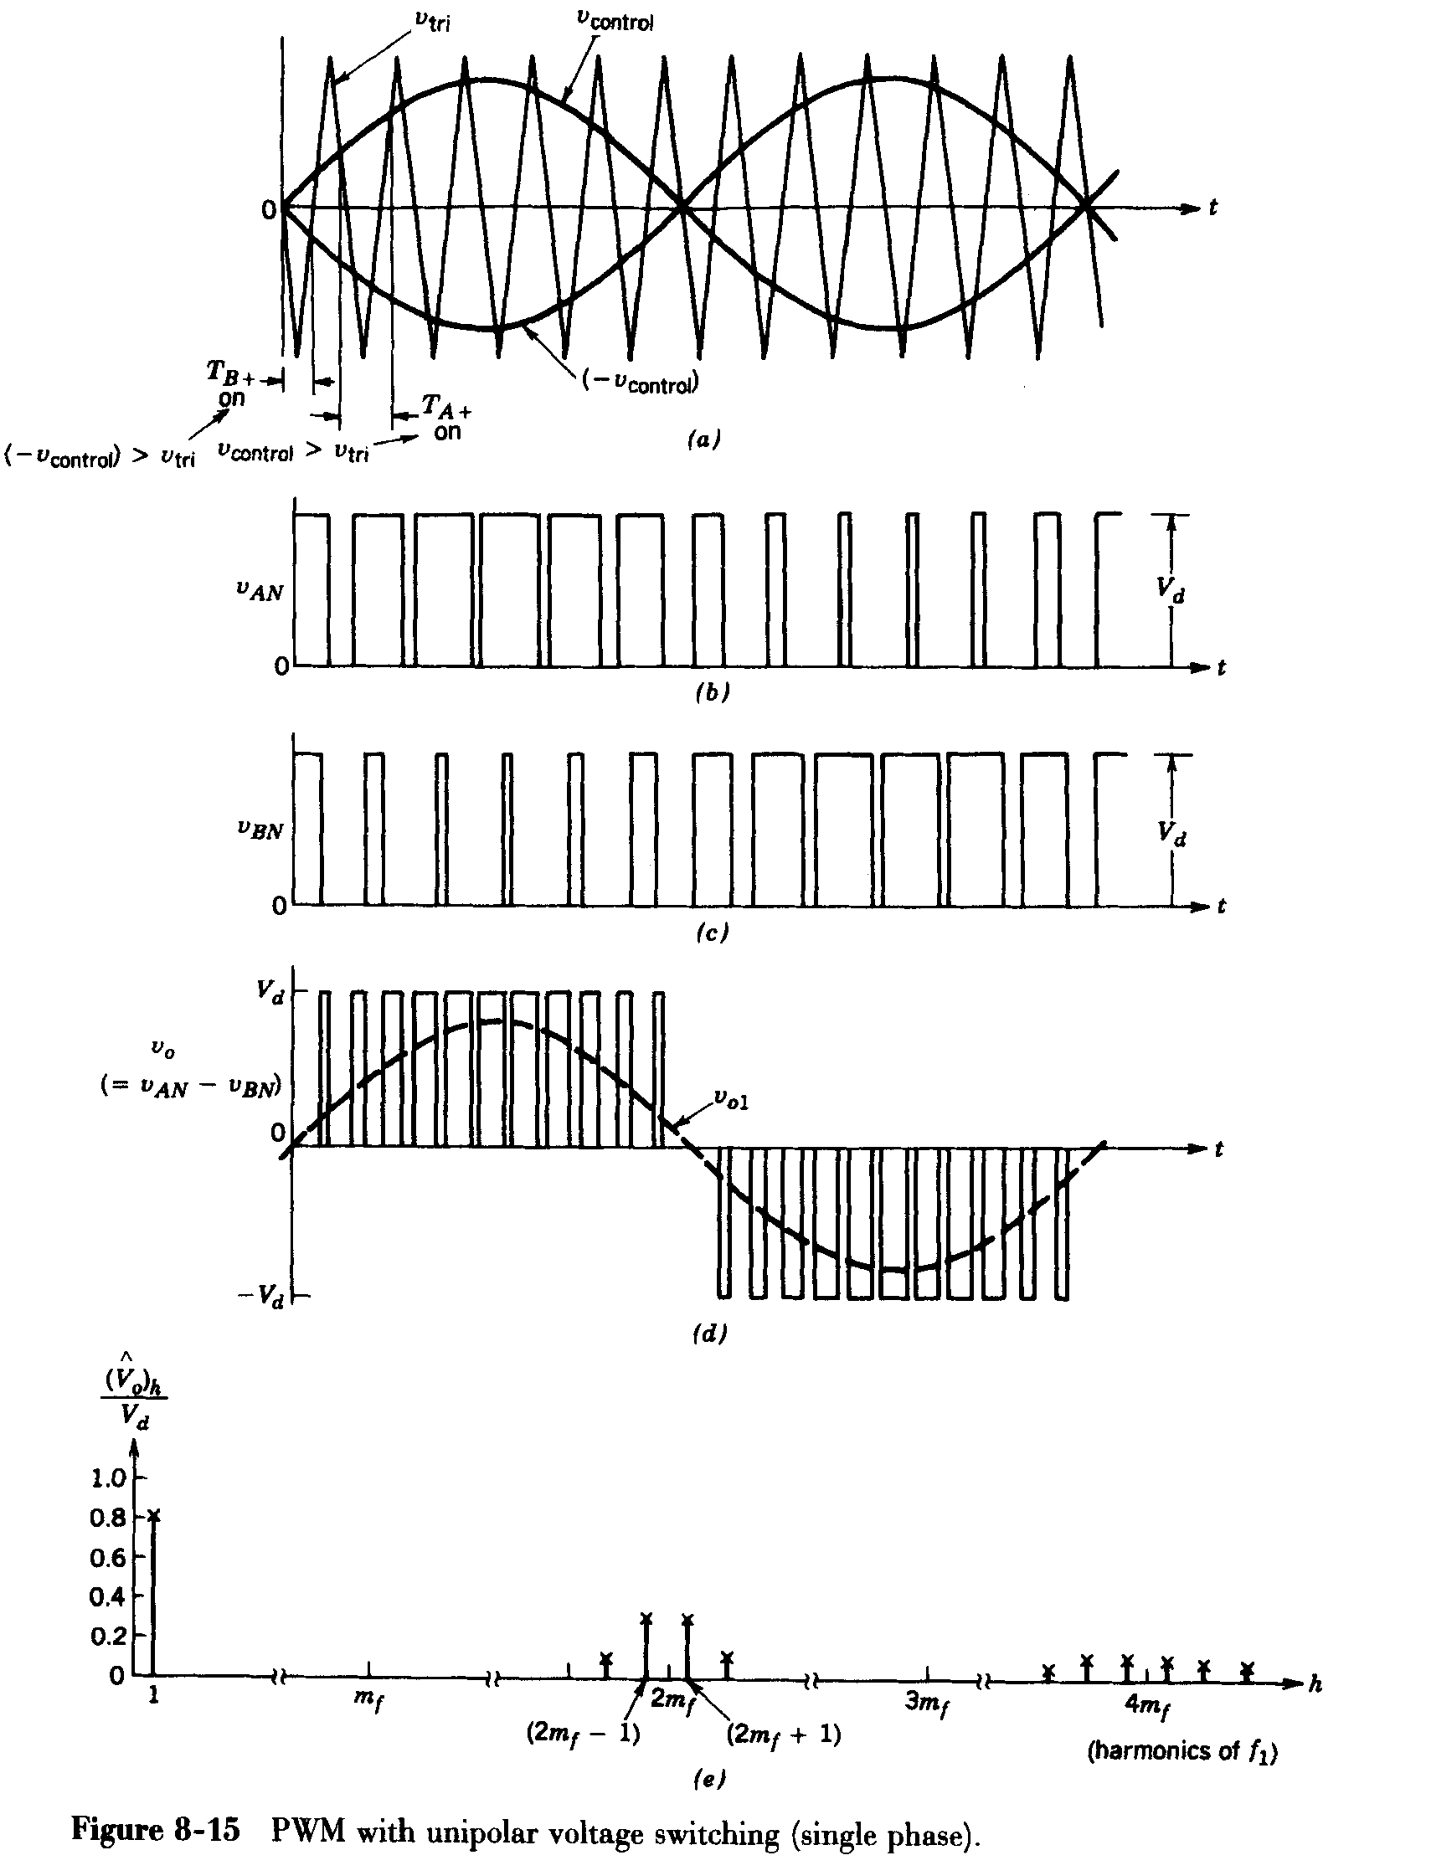
\includegraphics[width=0.72\textwidth]{mohan_fig_8_22_3ph_pwm_waveforms.png}
\caption{Three-phase PWM waveforms and harmonic spectrum: (a) Modulation references and carrier; (b) Pole voltages $v_{Ao}$ and $v_{Bo}$; (c) Line-to-line output voltage $v_{AB}(t) = v_{Ao} - v_{Bo}$; (d) Harmonic spectrum of line-to-line voltage showing total cancellation of all triplen harmonics ($3rd, 9th, 15th, \dots$). (Source: Ned Mohan, Fig.\ 8-22)}
\label{fig:3ph_pwm_waveforms}
\end{figure}

\subsubsection{Pole Voltages and Line-to-Line Voltages}
Each leg operates identically to a single-phase half-bridge pole relative to the fictitious DC-bus midpoint $o$:
\begin{equation}
v_{Ao}(t) = \begin{cases} +V_{dc}/2, & \text{if } v_{\text{control},A} > v_{\text{tri}} \\ -V_{dc}/2, & \text{if } v_{\text{control},A} < v_{\text{tri}} \end{cases}
\end{equation}
The line-to-line output voltages are obtained by taking the difference between individual leg pole voltages:
\begin{align}
v_{AB}(t) &= v_{Ao}(t) - v_{Bo}(t) \notag\\
v_{BC}(t) &= v_{Bo}(t) - v_{Co}(t) \notag\\
v_{CA}(t) &= v_{Co}(t) - v_{Ao}(t)
\end{align}

\subsubsection{Cancellation of Triplen Harmonics in Three-Phase PWM}
A fundamental property of three-phase balanced systems is that \textbf{all triplen harmonics ($n = 3, 9, 15, 21, \dots$) are identical in magnitude and in-phase across all three phase legs}:
\begin{equation}
v_{Ao,3}(t) = v_{Bo,3}(t) = v_{Co,3}(t)
\end{equation}
Taking the line-to-line difference completely cancels all triplen harmonics:
\begin{equation}
v_{AB,3}(t) = v_{Ao,3}(t) - v_{Bo,3}(t) \equiv 0!
\end{equation}
\begin{conceptbox}[Fundamental Voltage Relationships in 3-Phase SPWM]
In the linear modulation range ($0 \le m_a \le 1.0$):
\begin{enumerate}
  \item \textbf{Peak Fundamental Pole-to-Midpoint Voltage:}
  \begin{equation}
  \hat{V}_{Ao1} = m_a \frac{V_{dc}}{2}
  \end{equation}
  \item \textbf{Peak Fundamental Line-to-Line Voltage:}
  \begin{equation}
  \hat{V}_{LL1} = \sqrt{3} \hat{V}_{Ao1} = \sqrt{3} m_a \frac{V_{dc}}{2} = \frac{\sqrt{3}}{2} m_a V_{dc} \approx 0.866 m_a V_{dc}
  \label{eq:vll1_peak}
  \end{equation}
  \item \textbf{RMS Fundamental Line-to-Line Voltage:}
  \begin{equation}
  V_{LL1(rms)} = \frac{\hat{V}_{LL1}}{\sqrt{2}} = \frac{\sqrt{3}}{2\sqrt{2}} m_a V_{dc} = \frac{\sqrt{6}}{4} m_a V_{dc} \approx 0.6124 m_a V_{dc}
  \label{eq:vll1_rms}
  \end{equation}
  \item \textbf{Maximum Linear Line-to-Line RMS Voltage ($m_a = 1.0$):}
  \begin{equation}
  V_{LL1(rms),\text{max}} = 0.6124 V_{dc}
  \end{equation}
\end{enumerate}
\end{conceptbox}

\subsubsection{Three-Phase Frequency Modulation Ratio ($m_f$) Selection Criteria}
To ensure optimum harmonic elimination in three-phase inverters, $m_f$ must adhere to two strict design criteria:
\begin{enumerate}
  \item $m_f$ must be an \textbf{odd integer}: Ensures half-wave symmetry, completely eliminating all even harmonics.
  \item $m_f$ must be an \textbf{odd multiple of 3} ($m_f = 9, 15, 21, 27, 33, \dots$):
  \begin{itemize}
    \item Forces the dominant carrier-frequency harmonic cluster to appear at $m_f$ and its multiples.
    \item Because $m_f$ is a multiple of 3, this dominant harmonic cluster becomes a \textbf{triplen harmonic}, which is \textbf{completely cancelled out from the line-to-line voltage}!
    \item The lowest harmonic sidebands remaining in the line-to-line output voltage are pushed up to $(m_f \pm 2)$ and $(m_f \pm 4)$.
  \end{itemize}
\end{enumerate}

\subsection{Overmodulation and Square-Wave Operation in Three-Phase Inverters}

\subsubsection{Overmodulation Region ($1.0 < m_a \le 3.24$)}
When $m_a$ exceeds $1.0$, the peak reference wave exceeds the carrier amplitude. The fundamental line-to-line output voltage increases beyond $0.6124 V_{dc}$, but non-linear saturation occurs and low-order non-triplen harmonics (5th, 7th, 11th, 13th) appear in the output.

\subsubsection{Square-Wave Operation ($m_a > 3.24$ / Six-Step Inverter)}
In the extreme limit, the inverter operates as a classical **six-step (square-wave) inverter**, where each switch conducts for $180^\circ$ per cycle.
\begin{itemize}[leftmargin=*]
  \item The line-to-line voltage is a six-step waveform alternating between $+V_{dc}, 0,$ and $-V_{dc}$.
  \item The Fourier series of the line-to-line voltage is:
  \begin{equation}
  v_{AB}(t) = \sum_{n=1,5,7,11,13,\dots}^{\infty} \frac{4V_{dc}}{n\pi} \cos\left(\frac{n\pi}{6}\right) \sin(n\omega t)
  \end{equation}
  Notice that for all triplen harmonics ($n = 3, 9, 15, \dots$), $\cos(n\pi/6) = 0$, confirming complete triplen elimination!
  \item \textbf{Peak Fundamental Line-to-Line Voltage:}
  \begin{equation}
  \hat{V}_{LL1,\text{square}} = \frac{4V_{dc}}{\pi} \cos\left(\frac{\pi}{6}\right) = \frac{4V_{dc}}{\pi} \frac{\sqrt{3}}{2} = \frac{2\sqrt{3}}{\pi}V_{dc} \approx 1.1026 V_{dc}
  \end{equation}
  \item \textbf{RMS Fundamental Line-to-Line Voltage in Square-Wave Mode:}
  \begin{equation}
  V_{LL1(rms),\text{square}} = \frac{\hat{V}_{LL1,\text{square}}}{\sqrt{2}} = \frac{\sqrt{6}}{\pi}V_{dc} \approx 0.7797 V_{dc}
  \end{equation}
  \item \textbf{Total RMS Value of Line-to-Line Voltage:}
  \begin{equation}
  V_{LL(rms)} = \sqrt{\frac{1}{\pi} \int_0^{2\pi/3} V_{dc}^2 d(\omega t)} = V_{dc}\sqrt{\frac{2}{3}} \approx 0.8165 V_{dc}
  \end{equation}
\end{itemize}

\subsection{Third Harmonic Injection PWM (THIPWM)}

In standard sinusoidal PWM, the maximum linear fundamental line-to-line voltage is limited to $\hat{V}_{LL1} = \frac{\sqrt{3}}{2}V_{dc} \approx 0.866 V_{dc}$ because the peak of each phase reference sine wave cannot exceed the DC rails ($\pm V_{dc}/2$) without causing overmodulation distortion.

\begin{figure}[htbp]
\centering
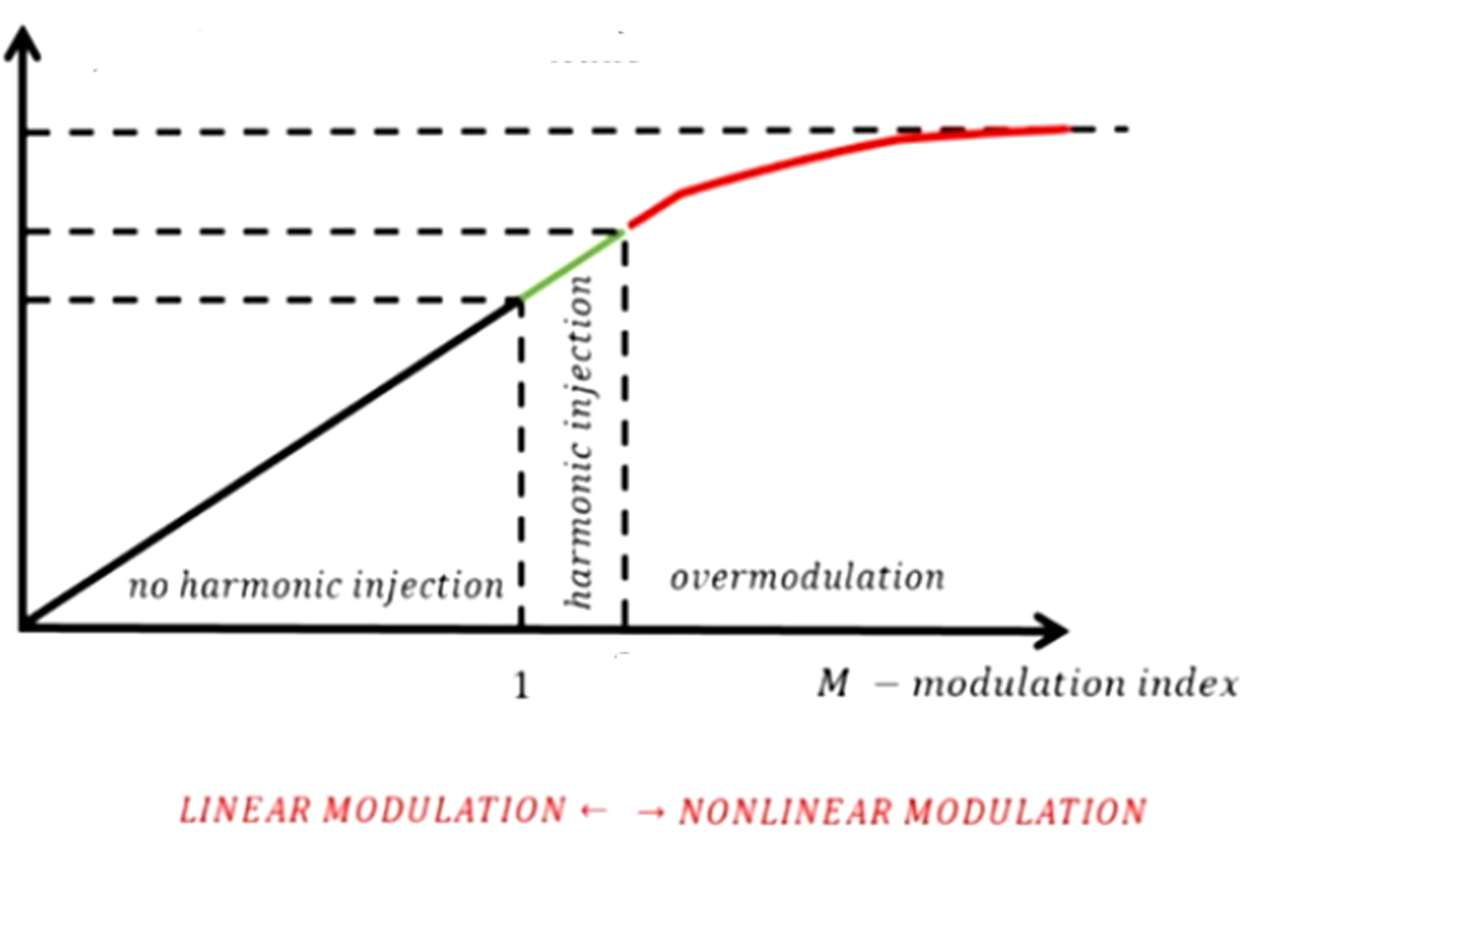
\includegraphics[width=0.68\textwidth]{mod_p52_img1.jpeg}
\caption{Third Harmonic Injection PWM (THIPWM): Addition of a 3rd harmonic zero-sequence component ($\frac{1}{6}\hat{V}_m \sin 3\omega t$) flattens the reference waveform peak, preventing carrier clipping while boosting DC bus utilization by $15.5\%$. (Source: CET Lecture Slides)}
\label{fig:thipwm}
\end{figure}

\subsubsection{Mathematical Formulation of THIPWM}
By adding a triplen zero-sequence third-harmonic component to the fundamental sinusoidal reference:
\begin{equation}
v_{\text{control},A}(t) = \hat{V}_1 \left[ \sin(\omega t) + \frac{1}{6} \sin(3\omega t) \right]
\label{eq:thipwm_formula}
\end{equation}
The optimal amplitude of the injected third harmonic is exactly $\frac{1}{6} \approx 16.7\%$ of the fundamental amplitude.

\subsubsection{Why Third Harmonic Injection Works}
\begin{conceptbox}[Physics of Third Harmonic Injection]
\begin{enumerate}
  \item \textbf{Peak Flattening:} At $\omega t = \pi/2$ ($90^\circ$), where $\sin(\omega t) = 1$, the third harmonic evaluates to $\sin(3 \cdot \pi/2) = \sin(270^\circ) = -1$. The reference voltage becomes:
  \begin{equation}
  v_{\text{control}}(\pi/2) = \hat{V}_1 \left[ 1 - \frac{1}{6} \right] = \frac{5}{6} \hat{V}_1
  \end{equation}
  The peak of the reference waveform is \textbf{flattened by a factor of $\frac{\sqrt{3}}{2} \approx 0.866$}!
  \item \textbf{15.5\% Voltage Boost in Linear Range:} Because the peak is flattened, the fundamental reference amplitude $\hat{V}_1$ can be boosted by $\frac{2}{\sqrt{3}} \approx 1.1547$ ($+15.47\%$) before the waveform touches the carrier peak!
  \begin{equation}
  \hat{V}_{LL1,\text{max (THIPWM)}} = 1.1547 \times 0.866 V_{dc} = 1.000 V_{dc}
  \end{equation}
  \begin{equation}
  V_{LL1(rms),\text{max (THIPWM)}} = \frac{V_{dc}}{\sqrt{2}} \approx 0.707 V_{dc}
  \end{equation}
  This represents an immense **$15.5\%$ increase in output voltage** compared to standard SPWM ($0.707 V_{dc}$ vs $0.612 V_{dc}$) without leaving the linear modulation region!
  \item \textbf{Zero Distortion Across Load:} Because the three phases are identical and balanced, the injected third harmonic components across phase legs $A, B,$ and $C$ are in-phase and cancel completely in the line-to-line voltage:
  \begin{equation}
  v_{AB}(t) = v_{Ao}(t) - v_{Bo}(t) = \text{Pure fundamental without any 3rd harmonic!}
  \end{equation}
  \item \textbf{Equivalence to Space Vector PWM (SVPWM):} Third harmonic injection PWM produces line-to-line voltage waveforms and DC bus utilization virtually identical to Space Vector Modulation (SVM), but with the computational simplicity of carrier-based analog/digital comparators!
\end{enumerate}
\end{conceptbox}


\section{Current Source Inverters (CSI) and Detailed Comparison with VSI}

\subsection{Operating Principle of Single-Phase Current Source Inverters (CSI)}

In contrast to a Voltage Source Inverter (which is fed from a stiff, low-impedance DC voltage source), a \textbf{Current Source Inverter (CSI)} is fed from an adjustable direct current source possessing \textbf{high internal impedance}. In practice, this is realized by placing a large smoothing choke ($L_{dc}$) in series with a controlled DC power supply or phase-controlled thyristor rectifier.

\begin{figure}[htbp]
\centering
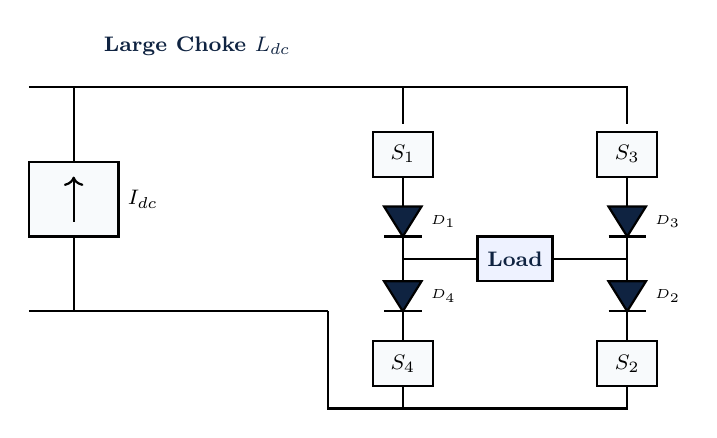
\begin{tikzpicture}[scale=0.95, every node/.style={transform shape}]
  % DC Current Source representation
  \draw[thick] (0, 3.5) -- (1.5, 3.5);
  \draw[thick] (0, 0.5) -- (1.5, 0.5);
  \draw[thick, fill=cardbg] (0, 1.5) rectangle (1.2, 2.5);
  \draw[thick, ->] (0.6, 1.7) -- (0.6, 2.3);
  \node[right, font=\footnotesize\bfseries] at (1.2, 2.0) {$I_{dc}$};
  \draw[thick] (0.6, 3.5) -- (0.6, 2.5);
  \draw[thick] (0.6, 0.5) -- (0.6, 1.5);
  
  % Large DC Inductor
  \draw[thick] (1.5, 3.5) to[decoration={coil,aspect=0.5,segment length=2mm,amplitude=2.5mm},decorate] (3.0, 3.5);
  \node[above, font=\footnotesize\bfseries, color=navyprimary] at (2.25, 3.8) {Large Choke $L_{dc}$};
  \draw[thick] (3.0, 3.5) -- (4.0, 3.5);
  \draw[thick] (1.5, 0.5) -- (4.0, 0.5);
  
  % H-Bridge Switches with Series Diodes
  % Leg 1: S1, D1 and S4, D4
  \draw[thick] (4.0, 3.5) -- (5.0, 3.5) -- (5.0, 3.0);
  % Switch S1
  \draw[thick, fill=cardbg] (4.6, 2.3) rectangle (5.4, 2.9);
  \node[font=\footnotesize\bfseries] at (5.0, 2.6) {$S_1$};
  % Diode D1
  \draw[thick] (5.0, 2.3) -- (5.0, 1.9);
  \draw[thick, fill=navyprimary] (4.75, 1.9) -- (5.25, 1.9) -- (5.0, 1.5) -- cycle;
  \draw[thick] (4.75, 1.5) -- (5.25, 1.5);
  \node[right, font=\tiny\bfseries] at (5.25, 1.7) {$D_1$};
  \draw[thick] (5.0, 1.5) -- (5.0, 1.2);
  
  % Leg 2: S3, D3 and S2, D2
  \draw[thick] (5.0, 3.5) -- (8.0, 3.5) -- (8.0, 3.0);
  % Switch S3
  \draw[thick, fill=cardbg] (7.6, 2.3) rectangle (8.4, 2.9);
  \node[font=\footnotesize\bfseries] at (8.0, 2.6) {$S_3$};
  % Diode D3
  \draw[thick] (8.0, 2.3) -- (8.0, 1.9);
  \draw[thick, fill=navyprimary] (7.75, 1.9) -- (8.25, 1.9) -- (8.0, 1.5) -- cycle;
  \draw[thick] (7.75, 1.5) -- (8.25, 1.5);
  \node[right, font=\tiny\bfseries] at (8.25, 1.7) {$D_3$};
  \draw[thick] (8.0, 1.5) -- (8.0, 1.2);
  
  % Output Load Terminals
  \draw[thick] (5.0, 1.2) -- (6.0, 1.2);
  \draw[thick] (8.0, 1.2) -- (7.0, 1.2);
  \draw[thick, fill=formulabg] (6.0, 0.9) rectangle (7.0, 1.5);
  \node[font=\footnotesize\bfseries, color=navyprimary] at (6.5, 1.2) {Load};
  
  % Lower Switches
  % S4, D4
  \draw[thick] (5.0, 1.2) -- (5.0, 0.9);
  \draw[thick, fill=navyprimary] (4.75, 0.9) -- (5.25, 0.9) -- (5.0, 0.5) -- cycle;
  \draw[thick] (4.75, 0.5) -- (5.25, 0.5);
  \node[right, font=\tiny\bfseries] at (5.25, 0.7) {$D_4$};
  \draw[thick] (5.0, 0.5) -- (5.0, 0.1);
  \draw[thick, fill=cardbg] (4.6, -0.5) rectangle (5.4, 0.1);
  \node[font=\footnotesize\bfseries] at (5.0, -0.2) {$S_4$};
  \draw[thick] (5.0, -0.5) -- (5.0, -0.8) -- (4.0, -0.8) -- (4.0, 0.5);
  
  % S2, D2
  \draw[thick] (8.0, 1.2) -- (8.0, 0.9);
  \draw[thick, fill=navyprimary] (7.75, 0.9) -- (8.25, 0.9) -- (8.0, 0.5) -- cycle;
  \draw[thick] (7.75, 0.5) -- (8.25, 0.5);
  \node[right, font=\tiny\bfseries] at (8.25, 0.7) {$D_2$};
  \draw[thick] (8.0, 0.5) -- (8.0, 0.1);
  \draw[thick, fill=cardbg] (7.6, -0.5) rectangle (8.4, 0.1);
  \node[font=\footnotesize\bfseries] at (8.0, -0.2) {$S_2$};
  \draw[thick] (8.0, -0.5) -- (8.0, -0.8) -- (5.0, -0.8);
\end{tikzpicture}
\caption{Single-phase IGBT-based Current Source Inverter (CSI) with series blocking diodes and massive DC smoothing inductor $L_{dc}$.}
\label{fig:csi_circuit}
\end{figure}

\subsubsection{Circuit Characteristics of the CSI}
\begin{enumerate}[leftmargin=*]
  \item \textbf{Constant Input Current ($I_{dc}$):} Due to the large inductance $L_{dc}$, the DC link current cannot change instantaneously:
  \begin{equation}
  i_{dc}(t) \approx I_{dc} = \text{constant (ripple-free)}
  \end{equation}
  \item \textbf{Square-Wave Output Current Waveform:} Gating switch pair $(S_1, S_2)$ directs $+I_{dc}$ through the load, while gating $(S_3, S_4)$ directs $-I_{dc}$ through the load. The output current $i_o(t)$ is therefore a \textbf{clean square wave alternating between $+I_{dc}$ and $-I_{dc}$}.
  \item \textbf{Need for Series Blocking Diodes ($D_1 - D_4$):}
  \begin{itemize}
    \item Standard power MOSFETs and IGBTs have anti-parallel body diodes or low reverse-blocking voltage ratings ($< 20\text{ V}$).
    \item In a CSI, the load voltage is alternating AC, meaning the switches must withstand \textbf{large reverse voltages}.
    \item Fast-recovery diodes are placed strictly in \textbf{series} with each controlled switch to provide the necessary reverse voltage blocking capability!
  \end{itemize}
  \item \textbf{Inherent Short-Circuit Immunity:} In a VSI, accidental simultaneous conduction of upper and lower switches causes an explosive shoot-through short circuit. In sharp contrast, in a CSI, \textbf{simultaneous conduction of upper and lower switches merely circulates the constant DC current $I_{dc}$ without any current spike!}
  \item \textbf{Open-Circuit Danger:} In a CSI, an open circuit in the load or DC path is catastrophic ($L \frac{di}{dt} \to \infty$, generating thousands of volts of inductive overvoltage arc breakdown). An overlap period is mandatory during commutation!
\end{enumerate}

\subsection{Comprehensive Technical Comparison: VSI vs. CSI}

The comparison between Voltage Source Inverters and Current Source Inverters is a quintessential KTU university examination question (often awarded 6 to 9 marks). Table~\ref{tab:vsi_vs_csi} provides an exhaustive, multi-dimensional comparison.

\begin{table}[htbp]
\centering
\small
\caption{Definitive Technical Comparison: Voltage Source Inverter (VSI) vs. Current Source Inverter (CSI)}
\label{tab:vsi_vs_csi}
\begin{tabularx}{\textwidth}{l p{6.5cm} X}
\toprule
\textbf{Feature / Parameter} & \textbf{Voltage Source Inverter (VSI)} & \textbf{Current Source Inverter (CSI)} \\
\midrule
\textbf{DC Source Characteristic} & Stiff DC voltage source with very small internal impedance & Stiff DC current source with very high internal impedance \\
\textbf{Energy Storage Element} & Large DC-link capacitor bank ($C_{dc}$) across input terminals & Large DC-link smoothing inductor / choke ($L_{dc}$) in series \\
\textbf{Output Voltage Waveform} & Controlled square wave or PWM pulsed waveform (independent of load) & Determined entirely by load impedance and current \\
\textbf{Output Current Waveform} & Determined entirely by the connected load impedance & Pure square wave or PWM current waveform (independent of load) \\
\textbf{Freewheeling / Blocking Diodes} & Requires freewheeling diodes in \textbf{anti-parallel} with switches & Requires blocking diodes in \textbf{series} with switches \\
\textbf{Regeneration Capability} & Requires a four-quadrant dual converter or active front-end rectifier & Natural and simple: just reverse the DC voltage polarity while $I_{dc}$ remains unidirectional \\
\textbf{Short-Circuit Behavior} & Highly vulnerable: leg shoot-through creates catastrophic short circuit & Inherent short-circuit ride-through; fault current limited by $I_{dc}$ \\
\textbf{Open-Circuit Behavior} & Safe: open circuit causes no damage & Extremely hazardous: open-circuit produces destructive inductive $L \frac{di}{dt}$ voltage spikes \\
\textbf{Switching Overlap Requirements} & Strict \textbf{blanking time (dead-time)} mandatory to avoid shoot-through & Strict \textbf{overlap time} mandatory to avoid open-circuiting the DC choke \\
\textbf{Switch Ratings} & High current rating, unidirectional voltage blocking & High reverse voltage blocking capability required \\
\textbf{Dynamic Response} & Extremely fast (voltage switched instantaneously) & Slower due to large magnetic time constant of $L_{dc}$ \\
\textbf{Size, Weight \& Cost} & Compact and lightweight (uses electrolytic/film capacitors) & Bulky, heavy, and expensive due to massive iron-core DC reactor \\
\textbf{Primary Industrial Use} & General-purpose industrial VFDs, solar inverters, EV traction, UPS & High-power multi-megawatt synchronous motor drives, induction heating \\
\bottomrule
\end{tabularx}
\end{table}


\section{Utility Interface, Harmonics, IEEE 519 Standard, and Active PFC}

\subsection{Degradation of the Electric Utility Interface}

Conventional line-frequency diode rectifiers and phase-controlled thyristor converters feeding DC filter capacitors draw \textbf{highly non-sinusoidal, pulsed input currents} from the electric utility AC distribution grid. 

\begin{figure}[htbp]
\centering
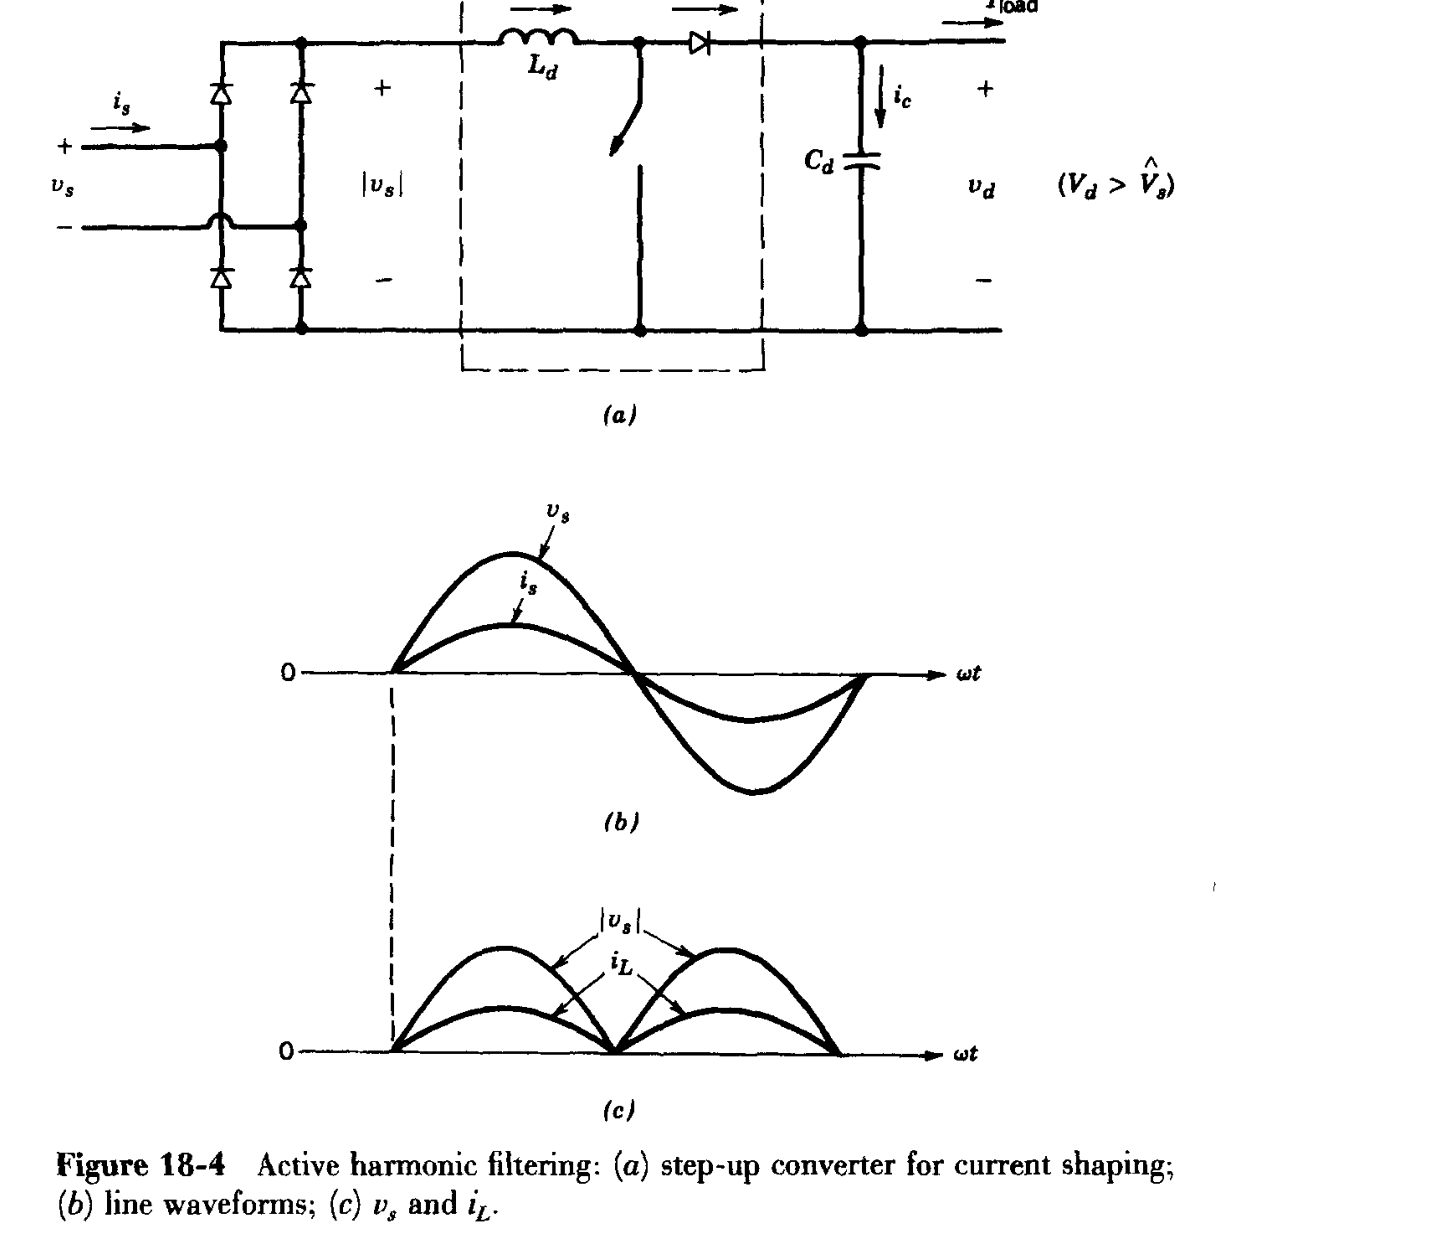
\includegraphics[width=0.68\textwidth]{mohan_fig_18_4_active_pfc.png}
\caption{Optimizing the utility interface: (a) Active power factor correction (PFC) step-up boost converter shaping the input current into a pure sinusoid in-phase with line voltage; (b) Input line current $i_s$, switch duty cycle, and high-frequency inductor current $i_L$. (Source: Ned Mohan, Fig.\ 18-4)}
\label{fig:active_pfc}
\end{figure}

\subsubsection{Harmonic Generation and Detrimental Impacts on Power Systems}
\begin{enumerate}[leftmargin=*]
  \item \textbf{Excessive Neutral Current in Three-Phase Four-Wire Systems:} Triplen current harmonics ($3rd, 9th, 15th, \dots$) generated by single-phase computer SMPS and electronic ballasts do not cancel in the neutral conductor; they add arithmetically in-phase:
  \begin{equation}
  I_N = \sqrt{I_{N,3}^2 + I_{N,9}^2 + \dots} \approx 3 \cdot I_{\text{phase},3}
  \end{equation}
  This causes neutral conductors to carry up to $1.73 - 2.0 \times$ the phase current, leading to transformer overheating and neutral cable fires!
  \item \textbf{Transformer and Generator De-rating:} High-frequency harmonic currents induce massive eddy current ($P_{\text{eddy}} \propto f^2$) and stray load losses in magnetic cores, requiring costly K-factor rated transformers.
  \item \textbf{Voltage Distortion Across the Power Grid:} The harmonic current $I_h$ drawn through the finite utility grid source impedance ($Z_s = R_s + j\omega L_s$) causes voltage drops that distort the supply voltage at the Point of Common Coupling (PCC):
  \begin{equation}
  V_{h,\text{PCC}} = I_h \cdot Z_{s,h}
  \end{equation}
  This degrades the voltage waveform delivered to neighboring consumers.
  \item \textbf{Harmonic Resonance with Power Factor Correction Capacitors:} Grid inductances and utility shunt capacitor banks form parallel resonant circuits ($f_{\text{res}} = \frac{1}{2\pi\sqrt{L_{\text{grid}} C_{\text{pfc}}}}$). Harmonic currents near $f_{\text{res}}$ excite catastrophic overvoltage resonances, exploding capacitor banks!
\end{enumerate}

\subsection{Power Factor in Non-Sinusoidal Circuits}

When the supply voltage is purely sinusoidal $v_s(t) = \sqrt{2}V_s \sin(\omega t)$ but the input current is distorted by non-linear electronics:
\begin{equation}
i_s(t) = \sqrt{2}I_{s1} \sin(\omega t - \phi_1) + \sum_{h=2}^{\infty} \sqrt{2}I_{sh} \sin(h\omega t - \phi_h)
\end{equation}
The total RMS current is given by:
\begin{equation}
I_s = \sqrt{I_{s1}^2 + \sum_{h=2}^\infty I_{sh}^2} = \sqrt{I_{s1}^2 + I_{\text{dist}}^2}
\end{equation}

\subsubsection{Active Real Power ($P$) and Apparent Power ($S$)}
Because the cross-product of orthogonal sinusoids of different frequencies integrates to zero over a full cycle, \textbf{only the fundamental current component $I_{s1}$ produces average real power}:
\begin{equation}
P = \frac{1}{T} \int_0^T v_s(t) i_s(t) dt = V_s I_{s1} \cos\phi_1
\end{equation}
The total apparent power is:
\begin{equation}
S = V_s I_s = V_s \sqrt{I_{s1}^2 + I_{\text{dist}}^2}
\end{equation}

\subsubsection{Displacement Power Factor (DPF) vs. Distortion Power Factor}
The true Power Factor (PF) is defined as the ratio of real active power to total apparent power:
\begin{equation}
\text{PF} = \frac{P}{S} = \frac{V_s I_{s1} \cos\phi_1}{V_s I_s} = \left(\frac{I_{s1}}{I_s}\right) \cdot \cos\phi_1
\end{equation}
\begin{formulabox}[True Power Factor Decomposition]
\begin{equation}
\text{PF} = K_{\text{dist}} \cdot \text{DPF} = \left(\frac{I_{s1}}{I_s}\right) \cos\phi_1
\label{eq:true_pf}
\end{equation}
where:
\begin{itemize}[leftmargin=*]
  \item $\text{DPF} = \cos\phi_1$ is the \textbf{Displacement Power Factor} (phase displacement of fundamental current relative to voltage).
  \item $K_{\text{dist}} = \frac{I_{s1}}{I_s}$ is the \textbf{Distortion Factor} (purity of the current waveform).
\end{itemize}
\end{formulabox}

\subsubsection{Relationship Between Distortion Factor and Total Harmonic Distortion (THD)}
The Total Harmonic Distortion of the current is defined as:
\begin{equation}
\text{THD}_i = \frac{\sqrt{\sum_{h=2}^\infty I_{sh}^2}}{I_{s1}} = \frac{\sqrt{I_s^2 - I_{s1}^2}}{I_{s1}} = \sqrt{\left(\frac{I_s}{I_{s1}}\right)^2 - 1}
\end{equation}
Rearranging gives the direct link between Distortion Factor and $\text{THD}_i$:
\begin{equation}
\frac{I_{s1}}{I_s} = \frac{1}{\sqrt{1 + \text{THD}_i^2}}
\end{equation}
Substituting into equation~\eqref{eq:true_pf} yields the foundational formula:
\begin{formulabox}[Master Formula: True Power Factor from THD]
\begin{equation}
\text{PF} = \frac{\cos\phi_1}{\sqrt{1 + \text{THD}_i^2}}
\label{eq:pf_from_thd}
\end{equation}
\end{formulabox}
\begin{conceptbox}[Crucial Exam Insight]
Even if the displacement power factor is unity ($\cos\phi_1 = 1.0$), a conventional bridge rectifier with a typical $\text{THD}_i = 80\%$ has a true power factor of only:
\begin{equation}
\text{PF} = \frac{1.0}{\sqrt{1 + (0.80)^2}} = \frac{1.0}{\sqrt{1 + 0.64}} = \frac{1.0}{1.2806} = 0.7808 \implies 78.1\%!
\end{equation}
This proves that **harmonic distortion alone degrades power factor**, regardless of capacitive/inductive phase shifts!
\end{conceptbox}

\subsection{IEEE 519 Standard for Harmonic Control in Electric Power Systems}

The **IEEE 519 Standard** (current revision IEEE 519-2022, "Standard for Harmonic Control in Electric Power Systems") establishes mandatory limits on harmonic distortion at the **Point of Common Coupling (PCC)** between an industrial or commercial customer and the utility transmission/distribution grid.

\subsubsection{PCC and Total Demand Distortion (TDD)}
IEEE 519 evaluates current distortion using **Total Demand Distortion (TDD)** rather than conventional THD:
\begin{equation}
\text{TDD} = \frac{\sqrt{\sum_{h=2}^\infty I_h^2}}{I_L}
\end{equation}
where $I_L$ is the **maximum demand load current** (fundamental frequency component of the maximum demand occurring over a 15-minute or 30-minute demand interval), while THD is calculated relative to instantaneous fundamental current $I_1$. Under light load, THD can be artificially astronomical ($>100\%$) while the actual harmonic Amperes injected into the grid are tiny; TDD prevents this distortion artifact!

\subsubsection{IEEE 519 Current Distortion Limits (for Systems Rated $120\text{ V}$ to $69\text{ kV}$)}
The permissible harmonic current limits depend directly on the **Short-Circuit Ratio (SCR)** at the PCC:
\begin{equation}
\text{SCR} = \frac{I_{sc}}{I_L}
\end{equation}
where $I_{sc}$ is the maximum short-circuit current available at the PCC, and $I_L$ is the maximum fundamental load demand current. A stiffer grid (higher $I_{sc}$) can absorb more harmonic current without suffering severe voltage distortion.

\begin{table}[htbp]
\centering
\small
\caption{IEEE 519 Current Distortion Limits at the PCC ($120\text{ V} - 69\text{ kV}$)}
\label{tab:ieee519_limits}
\begin{tabularx}{\textwidth}{c c c c c c Y}
\toprule
\textbf{$I_{sc} / I_L$ Ratio} & \textbf{$h < 11$} & \textbf{$11 \le h < 17$} & \textbf{$17 \le h < 23$} & \textbf{$23 \le h < 35$} & \textbf{$35 \le h \le 50$} & \textbf{Max TDD (\%)} \\
\midrule
$< 20^*$ & $4.0\%$ & $2.0\%$ & $1.5\%$ & $0.6\%$ & $0.3\%$ & $\mathbf{5.0\%}$ \\
$20 < 50$ & $7.0\%$ & $3.5\%$ & $2.5\%$ & $1.0\%$ & $0.5\%$ & $\mathbf{8.0\%}$ \\
$50 < 100$ & $10.0\%$ & $4.5\%$ & $4.0\%$ & $1.5\%$ & $0.7\%$ & $\mathbf{12.0\%}$ \\
$100 < 1000$ & $12.0\%$ & $5.5\%$ & $5.0\%$ & $2.0\%$ & $1.0\%$ & $\mathbf{15.0\%}$ \\
$> 1000$ & $15.0\%$ & $7.0\%$ & $6.0\%$ & $2.5\%$ & $1.4\%$ & $\mathbf{20.0\%}$ \\
\bottomrule
\multicolumn{7}{l}{\footnotesize *All power generation equipment is restricted to these lowest values regardless of actual $I_{sc}/I_L$.}
\end{tabularx}
\end{table}

\begin{table}[htbp]
\centering
\small
\caption{IEEE 519 Voltage Distortion Limits at the PCC}
\label{tab:ieee519_voltage}
\begin{tabularx}{\textwidth}{l c c}
\toprule
\textbf{Bus Voltage at PCC ($V$)} & \textbf{Individual Harmonic (\%)} & \textbf{Total Voltage Distortion $\text{THD}_v$ (\%)} \\
\midrule
$V \le 1.0\text{ kV}$ & $5.0\%$ & $\mathbf{8.0\%}$ \\
$1.0\text{ kV} < V \le 69\text{ kV}$ & $3.0\%$ & $\mathbf{5.0\%}$ \\
$69\text{ kV} < V \le 161\text{ kV}$ & $1.5\%$ & $\mathbf{2.5\%}$ \\
$V > 161\text{ kV}$ & $1.0\%$ & $\mathbf{1.5\%}$ \\
\bottomrule
\end{tabularx}
\end{table}

\subsection{Active Shaping of the Input Line Current (Power Factor Correction)}

To meet the rigorous harmonic constraints of IEEE 519 and IEC 61000-3-2, modern power supplies employ an **Active Power Factor Correction (PFC) Boost Converter** operating at high switching frequency ($50 - 200\text{ kHz}$) directly downstream of the uncontrolled diode bridge.

\begin{figure}[htbp]
\centering
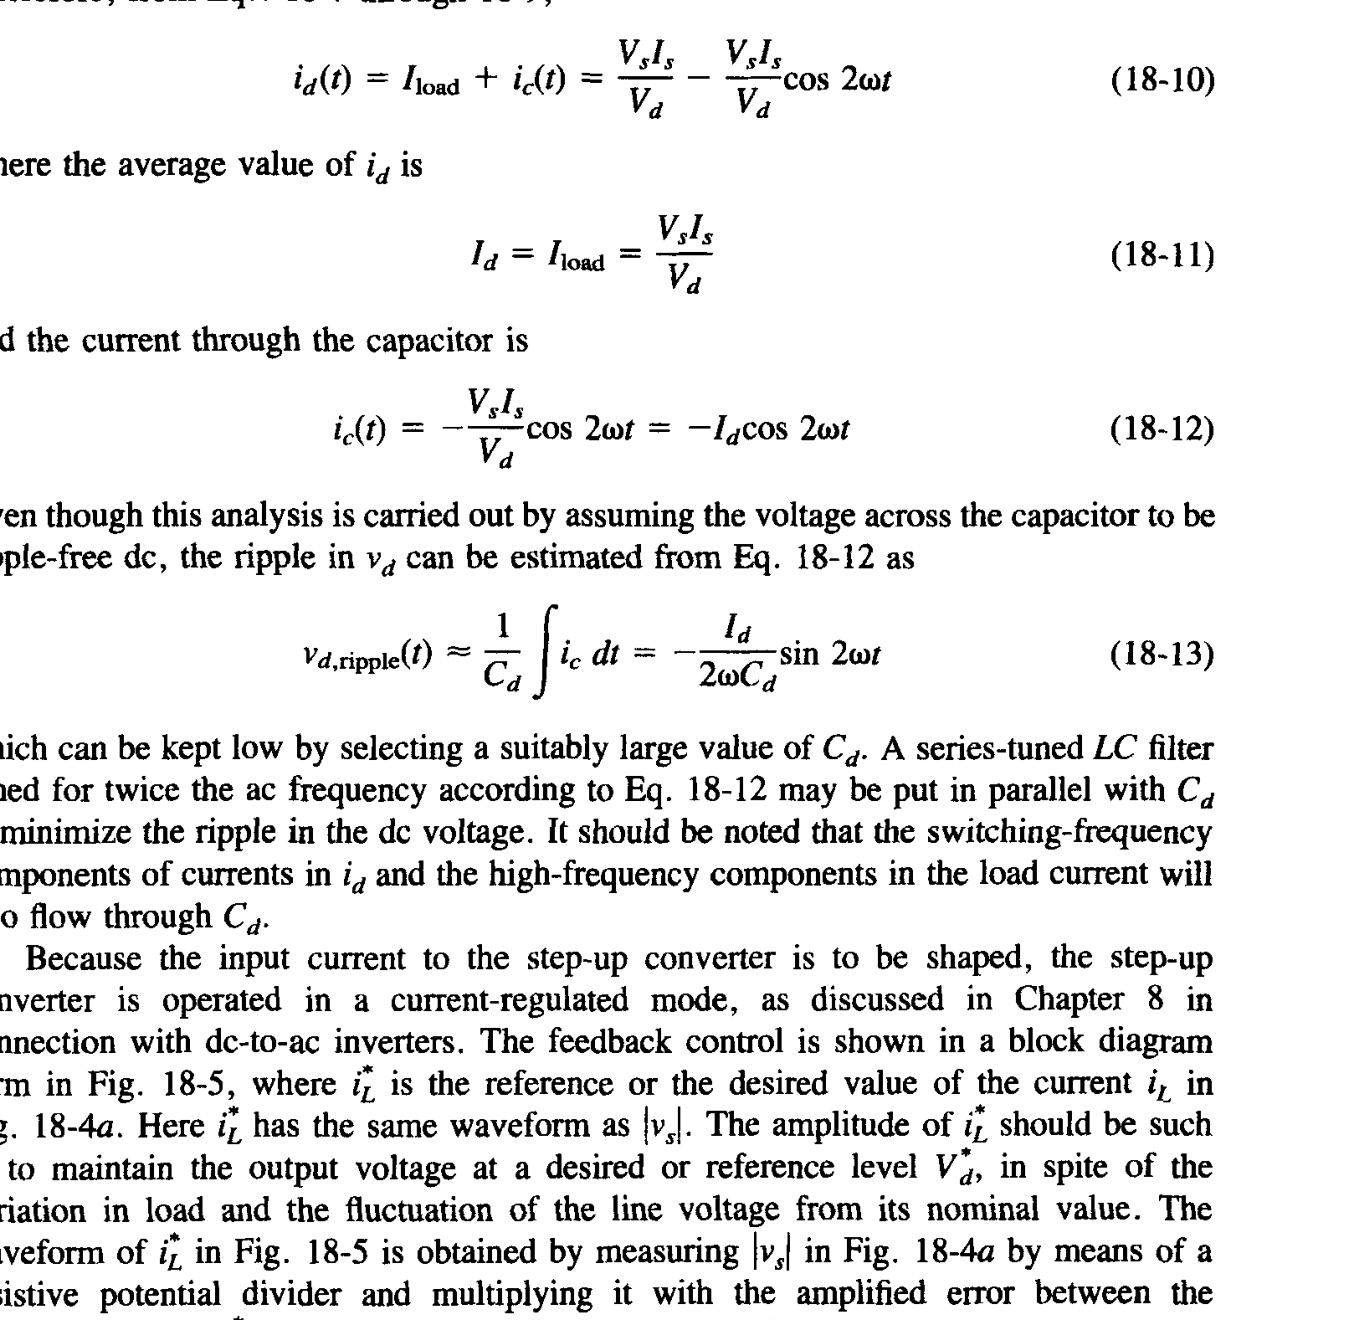
\includegraphics[width=0.72\textwidth]{mohan_fig_18_5_pfc_control.png}
\caption{Control architecture of an Active Power Factor Correction (PFC) boost converter: Outer voltage control loop regulating DC output voltage $V_d$, analog multiplier generating reference current $i_L^*$, and inner high-speed current loop driving PWM switch gate. (Source: Ned Mohan, Fig.\ 18-5)}
\label{fig:pfc_control}
\end{figure}

\subsubsection{Circuit Configuration and Dual-Loop Control Mechanics}
As depicted in Figures~\ref{fig:active_pfc} and~\ref{fig:pfc_control}, the active PFC step-up converter consists of a full-wave diode bridge, boost inductor $L$, power MOSFET/IGBT switch $S$, fast diode $D$, and DC bulk capacitor $C_d$.

The control system employs two cascaded feedback control loops:
\begin{enumerate}[leftmargin=*]
  \item \textbf{Slow Outer Voltage Loop (DC Bus Regulation):}
  \begin{itemize}
    \item Senses the DC link voltage $V_d$ and compares it to a precise reference $V_d^*$ (typically $390\text{ V} - 400\text{ V}$ DC for universal AC mains of $85\text{ V} - 265\text{ V}$).
    \item A proportional-integral (PI) voltage controller generates an error voltage signal $v_e$.
    \item \textbf{Deliberate Low Bandwidth:} The bandwidth of this loop is intentionally set very low ($10 - 20\text{ Hz}$) to prevent the controller from responding to the inevitable $100\text{ Hz}$ or $120\text{ Hz}$ ripple present on $V_d$.
  \end{itemize}

  \item \textbf{Analog Multiplier Stage:}
  \begin{itemize}
    \item Multiplies the slowly varying error signal $v_e$ with a rectified voltage template signal $|v_s(t)|$ obtained directly from a potential divider on the AC mains:
    \begin{equation}
    i_L^*(t) = K \cdot v_e \cdot |v_s(t)| = \hat{I}_L^* |\sin(\omega t)|
    \end{equation}
    This establishes an instantaneous reference current $i_L^*(t)$ that is guaranteed to have the exact same shape and phase as the AC mains voltage!
  \end{itemize}

  \item \textbf{Fast Inner Current Loop (Waveform Shaping):}
  \begin{itemize}
    \item Senses the instantaneous inductor current $i_L(t)$ using a shunt resistor or Hall-effect sensor.
    \item A high-bandwidth current controller (Average Current Mode Control or Peak Current Control) forces $i_L(t)$ to track $i_L^*(t)$ cycle-by-cycle at switching frequencies of $50 - 200\text{ kHz}$.
    \item When switch $S$ is closed: Inductor current rises ($di_L/dt = |v_s|/L$).
    \item When switch $S$ is open: Inductor current discharges into the load ($di_L/dt = (|v_s| - V_d)/L < 0$).
  \end{itemize}
\end{enumerate}

\subsubsection{Key Operating Metrics and Benefits of Active PFC}
\begin{itemize}[leftmargin=*]
  \item \textbf{Near-Unity Power Factor:} The input line current $i_s(t)$ is a clean, continuous sinusoid precisely in-phase with the line voltage ($\phi_1 \approx 0 \implies \text{DPF} \approx 1.0$).
  \item \textbf{Ultra-Low Harmonic Distortion:} $\text{THD}_i$ is suppressed from $>80\%$ down to $<3\% - 5\%$, easily satisfying IEEE 519 limits under all operating tiers!
  \item \textbf{Universal Input Voltage Range:} Active boost PFC automatically accommodates universal AC line inputs ($85\text{ V}_{\text{rms}} - 265\text{ V}_{\text{rms}}$, $47 - 63\text{ Hz}$) while maintaining a rock-steady regulated $400\text{ V}$ DC bus for downstream inverters or DC-DC stages!
\end{itemize}


\section{Ten Comprehensive University Exam Solved Numerical Problems}

\subsection{Problem 1: Single-Phase Full-Wave AC Voltage Controller with Resistive Load}
\begin{examplebox}[Problem 1: ACVC with $R$ Load Design \& Analysis]
\textbf{Statement:} A single-phase full-wave AC voltage controller is supplied from a $230\text{ V}$, $50\text{ Hz}$ single-phase source and feeds a purely resistive load of $R = 10\,\Omega$. The firing delay angle is set to $\alpha = \pi/3$ ($60^\circ$). Determine:
\begin{enumerate}
  \item The RMS output voltage $V_{or}$.
  \item The RMS load current $I_{or}$ and real active power dissipated in the load $P_o$.
  \item The input power factor $\text{PF}$.
  \item The average and RMS current ratings required for each individual thyristor.
\end{enumerate}

\tcblower
\textbf{Solution:}
\begin{enumerate}
  \item \textbf{RMS Output Voltage ($V_{or}$):}
  Using the master analytical formula for resistive load (equation~\eqref{eq:acvc_rms_r}):
  \begin{equation*}
  V_{or} = V_s \sqrt{1 - \frac{\alpha}{\pi} + \frac{\sin(2\alpha)}{2\pi}}
  \end{equation*}
  Here, $\alpha = \frac{\pi}{3} = 60^\circ$ ($1.0472\text{ rad}$), and $2\alpha = \frac{2\pi}{3} = 120^\circ$.
  \begin{equation*}
  \sin(2\alpha) = \sin(120^\circ) = \frac{\sqrt{3}}{2} \approx 0.8660
  \end{equation*}
  Substituting the numerical values into the square root expression:
  \begin{align*}
  \text{Term} &= 1 - \frac{\pi/3}{\pi} + \frac{0.8660}{2\pi} = 1 - \frac{1}{3} + \frac{0.8660}{6.2832} = \frac{2}{3} + 0.1378 = 0.6667 + 0.1378 = 0.8045 \notag\\
  \sqrt{0.8045} &\approx 0.8969
  \end{align*}
  Therefore, the RMS load voltage is:
  \begin{equation*}
  \mathbf{V_{or}} = 230 \times 0.8969 = \mathbf{206.3\text{ V}}
  \end{equation*}

  \item \textbf{RMS Load Current and Active Load Power:}
  \begin{equation*}
  \mathbf{I_{or}} = \frac{V_{or}}{R} = \frac{206.3\text{ V}}{10\,\Omega} = \mathbf{20.63\text{ A}}
  \end{equation*}
  The real power absorbed by the load resistor is:
  \begin{equation*}
  \mathbf{P_o} = I_{or}^2 \cdot R = (20.63)^2 \times 10 = \mathbf{4256\text{ W} = 4.256\text{ kW}}
  \end{equation*}

  \item \textbf{Input Power Factor ($\text{PF}$):}
  \begin{equation*}
  \mathbf{\text{PF}} = \frac{P_o}{V_s I_{or}} = \frac{V_{or}}{V_s} = \frac{206.3}{230} = \mathbf{0.897\text{ (lagging)}}
  \end{equation*}

  \item \textbf{Thyristor Current Ratings:}
  Each thyristor carries current for one half-cycle. Peak supply voltage is $V_m = \sqrt{2} \times 230 = 325.27\text{ V}$.
  \begin{align*}
  \mathbf{I_{T(avg)}} &= \frac{V_m}{2\pi R}(1 + \cos\alpha) = \frac{325.27}{2\pi \times 10}\left(1 + \cos 60^\circ\right) = \frac{32.527}{6.2832} (1 + 0.5) = 5.177 \times 1.5 = \mathbf{7.77\text{ A}} \notag\\
  \mathbf{I_{T(rms)}} &= \frac{I_{or}}{\sqrt{2}} = \frac{20.63}{\sqrt{2}} = \mathbf{14.59\text{ A}}
  \end{align*}
\end{enumerate}
\end{examplebox}

\subsection{Problem 2: Single-Phase AC Voltage Controller with Inductive $RL$ Load}
\begin{examplebox}[Problem 2: ACVC with $RL$ Load and Extinction Angle]
\textbf{Statement:} A $230\text{ V}$, $50\text{ Hz}$ single-phase AC voltage controller feeds a series $RL$ load with $R = 4\,\Omega$ and $\omega L = 3\,\Omega$. 
\begin{enumerate}
  \item Determine the minimum permissible firing angle $\alpha_{\text{min}}$ for controllable operation.
  \item For a firing angle $\alpha = 60^\circ$, if the numerical extinction angle is found to be $\beta = 220^\circ$ ($3.8397\text{ rad}$), calculate the conduction angle $\gamma$ and the RMS output voltage $V_{or}$.
\end{enumerate}

\tcblower
\textbf{Solution:}
\begin{enumerate}
  \item \textbf{Minimum Firing Angle ($\alpha_{\text{min}}$):}
  The load impedance magnitude and phase angle are:
  \begin{align*}
  Z &= \sqrt{R^2 + (\omega L)^2} = \sqrt{4^2 + 3^2} = \sqrt{16 + 9} = 5.0\,\Omega \notag\\
  \phi &= \arctan\left(\frac{\omega L}{R}\right) = \arctan\left(\frac{3}{4}\right) = 36.87^\circ = 0.6435\text{ rad}
  \end{align*}
  As established in Section 1, to maintain independent phase control and avoid current continuity breakdown, the firing delay angle must satisfy $\alpha \ge \phi$:
  \begin{equation*}
  \mathbf{\alpha_{\text{min}} = \phi = 36.87^\circ}
  \end{equation*}

  \item \textbf{Conduction Angle ($\gamma$) and RMS Output Voltage ($V_{or}$):}
  Given $\alpha = 60^\circ = \frac{\pi}{3}\text{ rad}$ ($1.0472\text{ rad}$) and $\beta = 220^\circ = 3.8397\text{ rad}$:
  \begin{equation*}
  \mathbf{\gamma} = \beta - \alpha = 220^\circ - 60^\circ = \mathbf{160^\circ = 2.7925\text{ rad}}
  \end{equation*}
  Using equation~\eqref{eq:acvc_rms_rl}:
  \begin{equation*}
  V_{or} = V_s \sqrt{\frac{1}{\pi} \left[ (\beta - \alpha) - \frac{\sin(2\beta) - \sin(2\alpha)}{2} \right]}
  \end{equation*}
  Evaluate the sinusoidal arguments:
  \begin{align*}
  2\beta &= 2 \times 220^\circ = 440^\circ = 80^\circ \implies \sin(440^\circ) = \sin(80^\circ) = 0.9848 \notag\\
  2\alpha &= 2 \times 60^\circ = 120^\circ \implies \sin(120^\circ) = 0.8660 \notag\\
  \frac{\sin(2\beta) - \sin(2\alpha)}{2} &= \frac{0.9848 - 0.8660}{2} = \frac{0.1188}{2} = 0.0594
  \end{align*}
  Now evaluate the term inside the square root:
  \begin{align*}
  \text{Term} &= \frac{1}{\pi} [2.7925 - 0.0594] = \frac{2.7331}{3.1416} = 0.8700 \notag\\
  \sqrt{\text{Term}} &= \sqrt{0.8700} \approx 0.9327
  \end{align*}
  Therefore, the RMS output voltage is:
  \begin{equation*}
  \mathbf{V_{or}} = 230 \times 0.9327 = \mathbf{214.5\text{ V}}
  \end{equation*}
\end{enumerate}
\end{examplebox}

\subsection{Problem 3: Single-Phase Full-Bridge Square-Wave Inverter Analysis}
\begin{examplebox}[Problem 3: Square-Wave Full-Bridge Inverter Analysis]
\textbf{Statement:} A single-phase full-bridge inverter is fed from a $48\text{ V}$ battery bank and delivers power to a series $RL$ load with $R = 5\,\Omega$ and $L = 20\text{ mH}$ operating at fundamental frequency $f = 50\text{ Hz}$. Determine:
\begin{enumerate}
  \item The total RMS output voltage $V_{or}$ and the fundamental RMS output voltage $V_{o1(rms)}$.
  \item The Fourier expression for the fundamental load current $i_{o1}(t)$ and its RMS magnitude $I_{o1(rms)}$.
  \item The fundamental active power $P_1$ absorbed by the load.
  \item The total harmonic distortion of the output voltage $\text{THD}_v$.
\end{enumerate}

\tcblower
\textbf{Solution:}
\begin{enumerate}
  \item \textbf{Output Voltages:}
  For a full-bridge square wave inverter:
  \begin{align*}
  \mathbf{V_{or}} &= V_{dc} = \mathbf{48.0\text{ V}} \notag\\
  \mathbf{V_{o1(rms)}} &= \frac{2\sqrt{2}}{\pi} V_{dc} = \frac{2\sqrt{2}}{\pi} \times 48 = 0.9003 \times 48 = \mathbf{43.21\text{ V}}
  \end{align*}
  Peak fundamental voltage: $\hat{V}_{o1} = \frac{4V_{dc}}{\pi} = \frac{4 \times 48}{\pi} = 61.12\text{ V}$.

  \item \textbf{Fundamental Load Current:}
  At $f = 50\text{ Hz}$, angular frequency $\omega = 2\pi \times 50 = 314.16\text{ rad/s}$.
  \begin{align*}
  X_{L1} &= \omega L = 314.16 \times 20 \times 10^{-3} = 6.283\,\Omega \notag\\
  Z_1 &= \sqrt{R^2 + X_{L1}^2} = \sqrt{5^2 + (6.283)^2} = \sqrt{25 + 39.48} = \sqrt{64.48} = 8.03\,\Omega \notag\\
  \phi_1 &= \arctan\left(\frac{6.283}{5}\right) = \arctan(1.2566) = 51.49^\circ = 0.8987\text{ rad}
  \end{align*}
  Peak fundamental load current:
  \begin{equation*}
  \hat{I}_{o1} = \frac{\hat{V}_{o1}}{Z_1} = \frac{61.12\text{ V}}{8.03\,\Omega} = 7.61\text{ A} \implies \mathbf{I_{o1(rms)}} = \frac{7.61}{\sqrt{2}} = \mathbf{5.38\text{ A}}
  \end{equation*}
  The instantaneous fundamental current expression is:
  \begin{equation*}
  \mathbf{i_{o1}(t) = 7.61 \sin(314.16 t - 51.49^\circ)\text{ A}}
  \end{equation*}

  \item \textbf{Fundamental Active Power ($P_1$):}
  \begin{equation*}
  \mathbf{P_1} = I_{o1(rms)}^2 \cdot R = (5.38)^2 \times 5 = 28.94 \times 5 = \mathbf{144.7\text{ W}}
  \end{equation*}

  \item \textbf{Total Harmonic Distortion ($\text{THD}_v$):}
  \begin{equation*}
  \mathbf{\text{THD}_v} = \sqrt{\frac{V_{or}^2 - V_{o1(rms)}^2}{V_{o1(rms)}^2}} = \sqrt{\left(\frac{48}{43.21}\right)^2 - 1} = \sqrt{1.2337 - 1} = \mathbf{48.34\%}
  \end{equation*}
\end{enumerate}
\end{examplebox}

\subsection{Problem 4: SPWM Full-Bridge Inverter with Bipolar Voltage Switching}
\begin{examplebox}[Problem 4: Bipolar SPWM Inverter Parameter Sizing]
\textbf{Statement:} A single-phase full-bridge inverter utilizing sinusoidal PWM with bipolar switching is supplied from a $V_{dc} = 300\text{ V}$ DC rail. The carrier frequency is $f_s = 2.0\text{ kHz}$ and the desired fundamental output frequency is $f_o = 50\text{ Hz}$. The amplitude of the triangular carrier is $\hat{V}_{\text{tri}} = 5\text{ V}$, and the amplitude of the control reference is $\hat{V}_{\text{control}} = 4\text{ V}$.
\begin{enumerate}
  \item Determine the amplitude modulation index $m_a$ and frequency modulation ratio $m_f$.
  \item Calculate the peak and RMS fundamental output voltages.
  \item Identify the frequencies of the first four dominant harmonic components in the output voltage.
\end{enumerate}

\tcblower
\textbf{Solution:}
\begin{enumerate}
  \item \textbf{Modulation Indices:}
  \begin{align*}
  \mathbf{m_a} &= \frac{\hat{V}_{\text{control}}}{\hat{V}_{\text{tri}}} = \frac{4\text{ V}}{5\text{ V}} = \mathbf{0.80} \notag\\
  \mathbf{m_f} &= \frac{f_s}{f_o} = \frac{2000\text{ Hz}}{50\text{ Hz}} = \mathbf{40}
  \end{align*}
  \textit{Design Note:} In practical design, $m_f$ would be selected as an odd integer (e.g., 39 or 41) to ensure half-wave symmetry and eliminate even harmonics.

  \item \textbf{Fundamental Output Voltages:}
  Since $m_a = 0.80 \le 1.0$, the inverter operates in the linear modulation range:
  \begin{align*}
  \mathbf{\hat{V}_{o1}} &= m_a \cdot V_{dc} = 0.80 \times 300\text{ V} = \mathbf{240.0\text{ V}} \notag\\
  \mathbf{V_{o1(rms)}} &= \frac{\hat{V}_{o1}}{\sqrt{2}} = \frac{240}{\sqrt{2}} = \mathbf{169.7\text{ V}}
  \end{align*}

  \item \textbf{Dominant Harmonic Frequencies:}
  For bipolar switching, harmonics appear as sidebands centered around $m_f$ and its multiples:
  \begin{itemize}
    \item Center harmonic: $f_{m_f} = m_f \cdot f_o = 40 \times 50 = \mathbf{2000\text{ Hz}}$.
    \item Sidebands around $m_f$: $(m_f \pm 2) f_o = (40 \pm 2) \times 50 \implies \mathbf{1900\text{ Hz}}$ and $\mathbf{2100\text{ Hz}}$.
    \item Sidebands around $2m_f$: $2m_f \cdot f_o = 4000\text{ Hz}$; sidebands at $(2m_f \pm 1) f_o \implies \mathbf{3950\text{ Hz}}$ and $\mathbf{4050\text{ Hz}}$.
  \end{itemize}
\end{enumerate}
\end{examplebox}

\subsection{Problem 5: SPWM Full-Bridge Inverter with Unipolar Voltage Switching}
\begin{examplebox}[Problem 5: Unipolar Switching vs. Bipolar Output Filter Sizing]
\textbf{Statement:} The inverter of Problem 4 is reconfigured to operate with **unipolar voltage switching** with the same DC link voltage ($V_{dc} = 300\text{ V}$), $m_a = 0.80$, and carrier frequency $f_s = 2\text{ kHz}$.
\begin{enumerate}
  \item Determine the peak and RMS fundamental output voltages.
  \item What is the lowest harmonic frequency present in the unipolar output voltage?
  \item If an $LC$ low-pass filter with corner frequency $f_c = \frac{1}{2\pi\sqrt{LC}}$ is designed to be one decade below the lowest harmonic frequency, calculate the required $LC$ product for both bipolar and unipolar PWM.
\end{enumerate}

\tcblower
\textbf{Solution:}
\begin{enumerate}
  \item \textbf{Fundamental Voltages:}
  The fundamental output voltage in unipolar switching is identical to bipolar switching:
  \begin{align*}
  \mathbf{\hat{V}_{o1}} &= m_a \cdot V_{dc} = 0.80 \times 300 = \mathbf{240\text{ V}} \notag\\
  \mathbf{V_{o1(rms)}} &= \frac{240}{\sqrt{2}} = \mathbf{169.7\text{ V}}
  \end{align*}

  \item \textbf{Lowest Harmonic Frequency:}
  In unipolar switching, all harmonics centered around $m_f$ ($2000\text{ Hz}$) cancel out! The first cluster appears around $2m_f$:
  \begin{equation*}
  f_{\text{lowest}} = (2m_f - 1) f_o = (80 - 1) \times 50 = 79 \times 50 = \mathbf{3950\text{ Hz}} \approx \mathbf{4.0\text{ kHz}}
  \end{equation*}

  \item \textbf{$LC$ Filter Product Comparison:}
  \begin{itemize}
    \item \textbf{Bipolar PWM:} Lowest harmonic occurs around $f_s = 2000\text{ Hz}$. One decade below gives filter cutoff $f_{c,\text{bipolar}} = 200\text{ Hz}$:
    \begin{equation*}
    (LC)_{\text{bipolar}} = \frac{1}{(2\pi f_{c,\text{bipolar}})^2} = \frac{1}{(2\pi \times 200)^2} = \frac{1}{(1256.6)^2} = \mathbf{6.33 \times 10^{-7}\text{ s}^2}
    \end{equation*}
    \item \textbf{Unipolar PWM:} Lowest harmonic occurs around $2f_s = 4000\text{ Hz}$. One decade below gives filter cutoff $f_{c,\text{unipolar}} = 400\text{ Hz}$:
    \begin{equation*}
    (LC)_{\text{unipolar}} = \frac{1}{(2\pi \times 400)^2} = \frac{1}{(2513.3)^2} = \mathbf{1.58 \times 10^{-7}\text{ s}^2}
    \end{equation*}
  \end{itemize}
  \textbf{Conclusion:} Unipolar switching allows a **$4 \times$ reduction in the $LC$ product**, dramatically reducing filter inductor weight, copper losses, and capacitor cost!
\end{enumerate}
\end{examplebox}

\subsection{Problem 6: Three-Phase PWM Voltage Source Inverter}
\begin{examplebox}[Problem 6: Three-Phase SPWM Line-to-Line Voltage Calculation]
\textbf{Statement:} A three-phase bridge inverter is supplied from an electric vehicle battery pack of $V_{dc} = 400\text{ V}$. The inverter is controlled using three-phase sinusoidal PWM in the linear modulation range with $m_a = 0.85$ and $m_f = 21$.
\begin{enumerate}
  \item Calculate the peak and RMS values of the fundamental phase-to-neutral (pole) voltage.
  \item Calculate the peak and RMS values of the fundamental line-to-line output voltage.
  \item Calculate the maximum achievable RMS fundamental line-to-line voltage in the linear range ($m_a = 1.0$), and compare it to the six-step square-wave mode.
\end{enumerate}

\tcblower
\textbf{Solution:}
\begin{enumerate}
  \item \textbf{Fundamental Phase Voltage ($v_{Ao1}$):}
  \begin{align*}
  \mathbf{\hat{V}_{Ao1}} &= m_a \frac{V_{dc}}{2} = 0.85 \times \frac{400}{2} = \mathbf{170.0\text{ V}} \notag\\
  \mathbf{V_{Ao1(rms)}} &= \frac{\hat{V}_{Ao1}}{\sqrt{2}} = \frac{170}{\sqrt{2}} = \mathbf{120.2\text{ V}}
  \end{align*}

  \item \textbf{Fundamental Line-to-Line Voltage ($V_{LL1}$):}
  Using equations~\eqref{eq:vll1_peak} and~\eqref{eq:vll1_rms}:
  \begin{align*}
  \mathbf{\hat{V}_{LL1}} &= \sqrt{3} \hat{V}_{Ao1} = \sqrt{3} \times 170.0\text{ V} = \mathbf{294.4\text{ V}} \notag\\
  \mathbf{V_{LL1(rms)}} &= \frac{\sqrt{6}}{4} m_a V_{dc} = 0.6124 \times 0.85 \times 400 = \mathbf{208.2\text{ V}}
  \end{align*}

  \item \textbf{Maximum Voltage Comparison:}
  \begin{itemize}
    \item \textbf{Maximum Linear SPWM ($m_a = 1.0$):}
    \begin{equation*}
    V_{LL1(rms),\text{max}} = 0.6124 \times 400\text{ V} = \mathbf{245.0\text{ V}}
    \end{equation*}
    \item \textbf{Six-Step Square-Wave Mode:}
    \begin{equation*}
    V_{LL1(rms),\text{square}} = \frac{\sqrt{6}}{\pi} V_{dc} = \frac{\sqrt{6}}{\pi} \times 400 = 0.7797 \times 400 = \mathbf{311.9\text{ V}}
    \end{equation*}
  \end{itemize}
  Operating in six-step mode yields $\frac{311.9}{245.0} = 1.273$ ($+27.3\%$) higher fundamental voltage than linear SPWM.
\end{enumerate}
\end{examplebox}

\subsection{Problem 7: Third Harmonic Injection PWM (THIPWM) Voltage Boost}
\begin{examplebox}[Problem 7: THIPWM DC Bus Utilization Advantage]
\textbf{Statement:} A 3-phase inverter fed by a $V_{dc} = 600\text{ V}$ DC bus supplies a $415\text{ V}$ (RMS line-to-line), $50\text{ Hz}$ three-phase induction motor.
\begin{enumerate}
  \item Determine if standard sinusoidal PWM in the linear range can deliver the required $415\text{ V}$ RMS line-to-line motor voltage.
  \item Calculate the maximum line-to-line RMS voltage achievable using Third Harmonic Injection PWM (THIPWM) while remaining strictly within the linear modulation boundary.
  \item Can THIPWM supply the motor at rated voltage without overmodulation?
\end{enumerate}

\tcblower
\textbf{Solution:}
\begin{enumerate}
  \item \textbf{Maximum Linear Voltage with Standard SPWM:}
  For standard SPWM, the maximum modulation index is $m_a = 1.0$:
  \begin{equation*}
  V_{LL1(rms),\text{max (SPWM)}} = 0.6124 \times V_{dc} = 0.6124 \times 600\text{ V} = \mathbf{367.4\text{ V}}
  \end{equation*}
  Since $367.4\text{ V} < 415\text{ V}$, \textbf{standard SPWM cannot provide the rated voltage} without entering severe overmodulation distortion!

  \item \textbf{Maximum Linear Voltage with THIPWM:}
  With optimal third harmonic injection ($v_3 = \frac{1}{6}\hat{V}_1 \sin 3\omega t$), the maximum fundamental voltage in the linear range is boosted by $\frac{2}{\sqrt{3}} \approx 1.1547$:
  \begin{equation*}
  \mathbf{V_{LL1(rms),\text{max (THIPWM)}}} = \frac{V_{dc}}{\sqrt{2}} = \frac{600\text{ V}}{\sqrt{2}} = \mathbf{424.26\text{ V}}
  \end{equation*}

  \item \textbf{Feasibility Assessment:}
  Since $424.26\text{ V} > 415\text{ V}$, \textbf{THIPWM comfortably delivers the rated $415\text{ V}$ output} with $m_a = \frac{415}{424.26} = 0.978 \le 1.0$, completely avoiding low-order harmonic distortion!
\end{enumerate}
\end{examplebox}

\subsection{Problem 8: Analytical Evaluation of Dead-Time (Blanking Time) Voltage Drop}
\begin{examplebox}[Problem 8: Dead-Time Induced Fundamental Voltage Reduction]
\textbf{Statement:} A high-power IGBT three-phase inverter operates from a $V_{dc} = 750\text{ V}$ DC bus with switching frequency $f_s = 10\text{ kHz}$. To prevent shoot-through, a blanking time of $t_d = 2.5\,\mu\text{s}$ is programmed into the gate drive controller.
\begin{enumerate}
  \item Calculate the average voltage error $\Delta V_o$ per phase leg.
  \item Determine the percentage reduction in fundamental output voltage if the inverter is operating at modulation index $m_a = 0.20$ (low-speed motor operation).
  \item Propose how this distortion can be compensated in industrial DSP motor drives.
\end{enumerate}

\tcblower
\textbf{Solution:}
\begin{enumerate}
  \item \textbf{Average Leg Voltage Error ($\Delta V_o$):}
  Using equation~\eqref{eq:deadtime_voltage_drop}:
  \begin{equation*}
  \mathbf{\Delta V_o} = 4 f_s t_d V_{dc} = 4 \times (10 \times 10^3\text{ Hz}) \times (2.5 \times 10^{-6}\text{ s}) \times 750\text{ V}
  \end{equation*}
  \begin{equation*}
  \mathbf{\Delta V_o} = 4 \times 0.025 \times 750 = 0.10 \times 750 = \mathbf{75.0\text{ V}}
  \end{equation*}

  \item \textbf{Percentage Voltage Reduction at $m_a = 0.20$:}
  Nominal fundamental peak pole voltage without dead time:
  \begin{equation*}
  \hat{V}_{Ao1} = m_a \frac{V_{dc}}{2} = 0.20 \times \frac{750}{2} = 75.0\text{ V}
  \end{equation*}
  The fundamental component of the dead-time error square wave is $\frac{4}{\pi}\Delta V_o$:
  \begin{equation*}
  \hat{V}_{\text{error},1} = \frac{4}{\pi} (f_s t_d V_{dc}) = \frac{4}{\pi} \times 18.75 = 23.87\text{ V}
  \end{equation*}
  Percentage fundamental loss:
  \begin{equation*}
  \mathbf{\% \text{ Loss}} = \frac{23.87\text{ V}}{75.0\text{ V}} \times 100\% = \mathbf{31.8\%!}
  \end{equation*}
  At low speeds ($m_a = 0.20$), dead-time causes an enormous $31.8\%$ drop in motor flux and severe 5th/7th torque pulsations!

  \item \textbf{Compensation Strategy:}
  DSP controllers implement **Dead-Time Compensation**: the controller detects the sign of the phase current ($i_A > 0$ or $i_A < 0$) using current sensors and dynamically adds or subtracts a pulse width correction $\Delta t = t_d$ to the PWM timer registers, completely restoring fundamental voltage linearity!
\end{enumerate}
\end{examplebox}

\subsection{Problem 9: Power Factor and THD in Non-Sinusoidal Rectifiers}
\begin{examplebox}[Problem 9: True Power Factor and Distortion Factor Evaluation]
\textbf{Statement:} A single-phase diode bridge rectifier with a capacitive filter draws a non-sinusoidal input current from a $230\text{ V}$, $50\text{ Hz}$ supply. A power quality analyzer records the fundamental current component as $I_{s1} = 10\text{ A}$ (RMS) lagging the line voltage by $\phi_1 = 18^\circ$, and harmonic current components of: $I_{s3} = 7.5\text{ A}$, $I_{s5} = 4.5\text{ A}$, $I_{s7} = 2.0\text{ A}$, and $I_{s9} = 1.0\text{ A}$ (higher harmonics negligible).
\begin{enumerate}
  \item Calculate the total RMS input current $I_s$.
  \item Compute the current Total Harmonic Distortion ($\text{THD}_i$).
  \item Determine the Distortion Factor ($K_{\text{dist}}$) and Displacement Power Factor ($\text{DPF}$).
  \item Calculate the True Power Factor ($\text{PF}$) and real active power drawn from the mains.
\end{enumerate}

\tcblower
\textbf{Solution:}
\begin{enumerate}
  \item \textbf{Total RMS Current ($I_s$):}
  \begin{align*}
  I_{\text{dist}}^2 &= \sum_{h=3,5,7,9} I_{sh}^2 = (7.5)^2 + (4.5)^2 + (2.0)^2 + (1.0)^2 = 56.25 + 20.25 + 4.0 + 1.0 = 81.5\text{ A}^2 \notag\\
  I_s &= \sqrt{I_{s1}^2 + I_{\text{dist}}^2} = \sqrt{10^2 + 81.5} = \sqrt{181.5} = \mathbf{13.47\text{ A}}
  \end{align*}

  \item \textbf{Current Total Harmonic Distortion ($\text{THD}_i$):}
  \begin{equation*}
  \mathbf{\text{THD}_i} = \frac{\sqrt{I_{\text{dist}}^2}}{I_{s1}} = \frac{\sqrt{81.5}}{10} = \frac{9.028}{10} = 0.9028 \implies \mathbf{90.28\%}
  \end{equation*}

  \item \textbf{Distortion Factor and Displacement Factor:}
  \begin{align*}
  \mathbf{K_{\text{dist}}} &= \frac{I_{s1}}{I_s} = \frac{10\text{ A}}{13.47\text{ A}} = \mathbf{0.7424} \notag\\
  \mathbf{\text{DPF}} &= \cos\phi_1 = \cos(18^\circ) = \mathbf{0.9511}
  \end{align*}

  \item \textbf{True Power Factor and Real Power:}
  Using equation~\eqref{eq:true_pf}:
  \begin{equation*}
  \mathbf{\text{PF}} = K_{\text{dist}} \times \text{DPF} = 0.7424 \times 0.9511 = \mathbf{0.706\text{ (lagging)}}
  \end{equation*}
  Verification using equation~\eqref{eq:pf_from_thd}:
  \begin{equation*}
  \text{PF} = \frac{\cos(18^\circ)}{\sqrt{1 + (0.9028)^2}} = \frac{0.9511}{\sqrt{1 + 0.815}} = \frac{0.9511}{\sqrt{1.815}} = \frac{0.9511}{1.3472} = 0.706\text{ (Exact match!)}
  \end{equation*}
  Real active power consumed:
  \begin{equation*}
  \mathbf{P} = V_s I_{s1} \cos\phi_1 = 230 \times 10 \times 0.9511 = \mathbf{2187.5\text{ W} = 2.188\text{ kW}}
  \end{equation*}
  Apparent power: $S = V_s I_s = 230 \times 13.47 = 3098\text{ VA}$. $\text{PF} = 2187.5 / 3098 = 0.706$.
\end{enumerate}
\end{examplebox}

\subsection{Problem 10: Active Power Factor Correction (PFC) Boost Converter Design}
\begin{examplebox}[Problem 10: Active PFC Boost Inductor Sizing \& IEEE 519 Check]
\textbf{Statement:} A $1.5\text{ kW}$ single-phase Active PFC boost converter is connected to a $230\text{ V}_{\text{rms}}$, $50\text{ Hz}$ AC line. The regulated DC bus voltage is $V_d = 400\text{ V}$, switching frequency is $f_s = 100\text{ kHz}$, and target converter efficiency is $\eta = 95\%$.
\begin{enumerate}
  \item Determine the peak and RMS fundamental input currents drawn from the AC line.
  \item Calculate the maximum peak-to-peak inductor ripple current $\Delta I_{L,\text{max}}$ if ripple is limited to $20\%$ of peak input current.
  \item Calculate the required boost inductance $L$.
  \item At the customer Point of Common Coupling (PCC), the available short-circuit current is $I_{sc} = 650\text{ A}$. What is the maximum permissible total demand distortion (TDD) specified by IEEE 519?
\end{enumerate}

\tcblower
\textbf{Solution:}
\begin{enumerate}
  \item \textbf{Input Line Currents:}
  Input active power drawn from the mains:
  \begin{equation*}
  P_{\text{in}} = \frac{P_{\text{out}}}{\eta} = \frac{1500\text{ W}}{0.95} = 1578.9\text{ W}
  \end{equation*}
  Since the PFC converter shapes current to achieve near-unity power factor ($\text{PF} \approx 1.0$):
  \begin{align*}
  \mathbf{I_{s(rms)}} &= \frac{P_{\text{in}}}{V_s} = \frac{1578.9\text{ W}}{230\text{ V}} = \mathbf{6.86\text{ A}} \notag\\
  \mathbf{\hat{I}_s} &= \sqrt{2} \times I_{s(rms)} = \sqrt{2} \times 6.86 = \mathbf{9.71\text{ A}}
  \end{align*}

  \item \textbf{Maximum Inductor Ripple Current ($\Delta I_{L,\text{max}}$):}
  \begin{equation*}
  \mathbf{\Delta I_{L,\text{max}}} = 20\% \times \hat{I}_s = 0.20 \times 9.71\text{ A} = \mathbf{1.942\text{ A}}
  \end{equation*}

  \item \textbf{Boost Inductance Sizing ($L$):}
  In a boost PFC converter, the duty cycle varies continuously across the line cycle: $d(t) = 1 - \frac{|v_s(t)|}{V_d}$. The ripple current is:
  \begin{equation*}
  \Delta i_L = \frac{|v_s| \cdot d}{f_s L} = \frac{|v_s|}{f_s L} \left(1 - \frac{|v_s|}{V_d}\right)
  \end{equation*}
  Differentiating with respect to $|v_s|$ shows that maximum ripple occurs precisely when $|v_s| = \frac{V_d}{2} = \frac{400}{2} = 200\text{ V}$ (where duty cycle $d = 0.5$):
  \begin{equation*}
  \Delta I_{L,\text{max}} = \frac{V_d / 2 \cdot 0.5}{f_s L} = \frac{V_d}{4 f_s L}
  \end{equation*}
  Rearranging to solve for inductance $L$:
  \begin{align*}
  \mathbf{L} &= \frac{V_d}{4 f_s \Delta I_{L,\text{max}}} = \frac{400\text{ V}}{4 \times (100 \times 10^3\text{ Hz}) \times 1.942\text{ A}} \notag\\
  &= \frac{400}{776,800} = 5.15 \times 10^{-4}\text{ H} = \mathbf{0.515\text{ mH} \approx 520\,\mu\text{H}}
  \end{align*}

  \item \textbf{IEEE 519 TDD Limit Evaluation:}
  The maximum fundamental load current is $I_L = I_{s(rms)} = 6.86\text{ A}$. The Short-Circuit Ratio (SCR) at the PCC is:
  \begin{equation*}
  \mathbf{\text{SCR}} = \frac{I_{sc}}{I_L} = \frac{650\text{ A}}{6.86\text{ A}} = \mathbf{94.75}
  \end{equation*}
  From Table~\ref{tab:ieee519_limits}, for $50 < \frac{I_{sc}}{I_L} < 100$:
  \begin{equation*}
  \mathbf{\text{Maximum Permissible TDD}} = \mathbf{12.0\%}
  \end{equation*}
  Since active PFC achieves $\text{THD}_i < 5\%$, the installation effortlessly complies with IEEE 519 with massive safety margins!
\end{enumerate}
\end{examplebox}


\section{Master Formula Sheet \& Quick Revision Tables}

\subsection{Master Analytical Formula Matrix}

\begin{table}[htbp]
\centering
\small
\caption{Module 3 Master Analytical Formula Cheat-Sheet for Fast Exam Revision}
\label{tab:module3_master_formulas}
\begin{tabularx}{\textwidth}{l p{5.5cm} X}
\toprule
\textbf{Topic / Circuit} & \textbf{Key Formulas / Governing Equations} & \textbf{Exam Tips \& Critical Insights} \\
\midrule
\textbf{ACVC ($R$ Load)} &
$V_{or} = V_s \sqrt{1 - \frac{\alpha}{\pi} + \frac{\sin 2\alpha}{2\pi}}$ \newline
$\text{PF} = \frac{V_{or}}{V_s} = \sqrt{1 - \frac{\alpha}{\pi} + \frac{\sin 2\alpha}{2\pi}}$ &
At $\alpha=0 \implies V_{or}=V_s, \text{PF}=1.0$. \newline
At $\alpha=90^\circ \implies V_{or}=0.707 V_s, \text{PF}=0.707$. \newline
At $\alpha=180^\circ \implies V_{or}=0, \text{PF}=0$. \\
\midrule
\textbf{ACVC ($RL$ Load)} &
$i_o(\omega t) = \frac{V_m}{Z}[\sin(\omega t-\phi) - \sin(\alpha-\phi)e^{-\frac{R}{\omega L}(\omega t-\alpha)}]$ \newline
$\sin(\beta-\phi) = \sin(\alpha-\phi)e^{-\frac{R}{\omega L}(\beta-\alpha)}$ \newline
$V_{or} = V_s \sqrt{\frac{1}{\pi}[(\beta-\alpha) - \frac{\sin 2\beta - \sin 2\alpha}{2}]}$ &
\textbf{Rule:} $\alpha \ge \phi = \arctan(\omega L / R)$. \newline
If $\alpha = \phi \implies \beta = \pi + \alpha \implies \gamma = 180^\circ$ (continuous sinusoidal current). \newline
Requires high-frequency pulse train gating! \\
\midrule
\textbf{ACVC (Integral Cycle)} &
$k = \frac{n}{n+m}$, \quad $V_{or} = V_s \sqrt{k}$ \newline
$\text{PF} = \sqrt{k}$ &
Zero switching EMI ($dv/dt=0, di/dt=0$). \newline
Causes line flicker/sub-harmonics. Used for thermal loads. \\
\midrule
\textbf{Half-Bridge VSI (Square Wave)} &
$v_o = \pm V_{dc}/2$, \quad $V_{or} = V_{dc}/2$ \newline
$\hat{V}_{o1} = \frac{2}{\pi}V_{dc}$, \quad $V_{o1(rms)} = \frac{\sqrt{2}}{\pi}V_{dc} \approx 0.45 V_{dc}$ &
Requires 3-wire DC split supply. \newline
Switch voltage rating $= V_{dc}$ ($2 \times$ peak output). \\
\midrule
\textbf{Full-Bridge VSI (Square Wave)} &
$v_o = \pm V_{dc}$, \quad $V_{or} = V_{dc}$ \newline
$\hat{V}_{o1} = \frac{4}{\pi}V_{dc}$, \quad $V_{o1(rms)} = \frac{2\sqrt{2}}{\pi}V_{dc} \approx 0.90 V_{dc}$ \newline
$\text{THD}_v = \sqrt{\frac{\pi^2}{8}-1} = 48.34\%$ &
Odd harmonics only ($n=1, 3, 5, 7, \dots$). \newline
Harmonic amplitude $\hat{V}_{on} = \hat{V}_{o1}/n$. \newline
Twice the voltage, $4\times$ power of half-bridge! \\
\midrule
\textbf{Single-Phase Bipolar SPWM} &
$m_a = \frac{\hat{V}_{\text{control}}}{\hat{V}_{\text{tri}}}$, \quad $m_f = \frac{f_s}{f_o}$ \newline
$\hat{V}_{o1} = m_a V_{dc}$, \quad $V_{o1(rms)} = \frac{m_a V_{dc}}{\sqrt{2}}$ &
$m_f$ must be an odd integer (eliminates even harmonics). \newline
Lowest harmonics clustered at $m_f \pm 2$. \\
\midrule
\textbf{Single-Phase Unipolar SPWM} &
$\hat{V}_{o1} = m_a V_{dc}$, \quad $V_{o1(rms)} = \frac{m_a V_{dc}}{\sqrt{2}}$ \newline
Effective switching frequency $= 2f_s$ &
3-level output ($+V_{dc}, 0, -V_{dc}$). \newline
Harmonics around $m_f$ cancel! First cluster at $2m_f$. \newline
$LC$ filter product reduced by $4\times$! \\
\midrule
\textbf{Three-Phase SPWM (Linear)} &
$\hat{V}_{Ao1} = m_a \frac{V_{dc}}{2}$ \newline
$\hat{V}_{LL1} = \frac{\sqrt{3}}{2} m_a V_{dc} \approx 0.866 m_a V_{dc}$ \newline
$V_{LL1(rms)} = \frac{\sqrt{6}}{4} m_a V_{dc} \approx 0.6124 m_a V_{dc}$ &
Triplen harmonics ($3rd, 9th, 15th, \dots$) cancel in line-line! \newline
Choose $m_f$ as an odd multiple of 3 ($9, 15, 21, \dots$). \newline
Max linear RMS line voltage $= 0.6124 V_{dc}$. \\
\midrule
\textbf{Three-Phase Six-Step (Square)} &
$V_{LL(rms)} = \sqrt{\frac{2}{3}}V_{dc} \approx 0.8165 V_{dc}$ \newline
$V_{LL1(rms)} = \frac{\sqrt{6}}{\pi}V_{dc} \approx 0.7797 V_{dc}$ &
$180^\circ$ conduction. Output contains $n=6k \pm 1$ ($5th, 7th, 11th$). \newline
Fundamental is $27.3\%$ higher than max linear SPWM. \\
\midrule
\textbf{Third Harmonic Injection (THIPWM)} &
$v_{\text{control}} = \hat{V}_1 [\sin(\omega t) + \frac{1}{6}\sin(3\omega t)]$ \newline
$V_{LL1(rms),\text{max}} = \frac{V_{dc}}{\sqrt{2}} \approx 0.707 V_{dc}$ &
Flattens sine peak by $0.866$. \newline
\textbf{Boosts linear output voltage by 15.5\%!} \newline
Third harmonic cancels out in line-to-line output! \\
\midrule
\textbf{Blanking Time (Dead-Time)} &
$\Delta V_o = 4 f_s t_d V_{dc}$ &
Prevents DC link shoot-through. \newline
Reduces fundamental voltage, distorts zero-crossings. \\
\midrule
\textbf{Harmonics \& Power Factor} &
$\text{PF} = \left(\frac{I_{s1}}{I_s}\right) \cos\phi_1 = \frac{\cos\phi_1}{\sqrt{1 + \text{THD}_i^2}}$ \newline
$\text{THD}_i = \frac{\sqrt{I_s^2 - I_{s1}^2}}{I_{s1}}$ &
True PF $=$ Distortion Factor $\times$ Displacement Factor. \newline
Harmonics alone reduce power factor even if $\cos\phi_1 = 1.0$! \\
\midrule
\textbf{Active PFC Boost Inductor} &
$\Delta I_{L,\text{max}} = \frac{V_d}{4 f_s L} \implies L = \frac{V_d}{4 f_s \Delta I_{L,\text{max}}}$ &
Max ripple occurs at $d=0.5$ ($|v_s| = V_d/2$). \newline
Universal AC input, regulates $V_d \approx 400\text{ V}$ DC, $\text{THD}_i < 5\%$. \\
\bottomrule
\end{tabularx}
\end{table}

\subsection{Essential Examination Quick-Tips for KTU S5 EEE Students}
\begin{enumerate}[leftmargin=*]
  \item \textbf{When asked for ACVC RMS Voltage Derivation:} Always state the half-wave symmetry condition ($v_o(\omega t + \pi) = -v_o(\omega t)$), integrate $[V_m \sin\omega t]^2$ from $\alpha$ to $\pi$ (or $\alpha$ to $\beta$ for $RL$ load), convert $\sin^2\theta = \frac{1 - \cos 2\theta}{2}$, and show every intermediate integration step clearly to secure full marks.
  \item \textbf{Why $\alpha < \phi$ is prohibited in $RL$ ACVC:} Remember the physical mechanism: If $\alpha < \phi$, the current in the previous thyristor is still flowing when the next thyristor is triggered. Conduction becomes continuous, phase control is completely lost, and the converter acts as a short circuit directly connecting the load to the AC mains.
  \item \textbf{Fourier Series of Square Wave Inverter:} Write down the general half-wave symmetry property first. State why all even harmonics and DC term are zero ($a_0 = 0, a_n = 0, b_{\text{even}} = 0$). Write the general formula $\sum \frac{4V_{dc}}{n\pi}\sin(n\omega t)$ and calculate $\text{THD}_v = \sqrt{\frac{\pi^2}{8}-1} = 48.34\%$.
  \item \textbf{Bipolar vs. Unipolar PWM Comparison:} Draw the two-level vs. three-level output waveforms side-by-side. Highlight the three killer facts: (1) Effective switching frequency doubles to $2f_s$; (2) Harmonics around $m_f$ cancel out completely; (3) Output filter size drops by $4\times$.
  \item \textbf{Why Triplen Harmonics Disappear in 3-Phase Inverters:} State that triplen harmonics ($3rd, 9th, 15th, \dots$) form a zero-sequence set—they are exactly equal in magnitude and in phase in all three inverter legs ($v_{Ao,3} = v_{Bo,3} = v_{Co,3}$). When computing line-to-line voltage $v_{AB} = v_{Ao} - v_{Bo}$, they subtract to exactly zero!
  \item \textbf{Dead-Time Derivation:} Draw the leg diagram showing $S_1, S_4$ and diodes $D_1, D_4$. Explain that when both switches are off during $t_d$, the load current $i_o$ forces either $D_1$ or $D_4$ to conduct depending solely on the sign of $i_o$, subtracting or adding volt-seconds to the output pulse.
  \item \textbf{IEEE 519 PCC Rule:} Remember that IEEE 519 applies strictly at the \textbf{Point of Common Coupling (PCC)}, NOT inside the customer plant. Limits are specified in terms of \textbf{Total Demand Distortion (TDD)} and depend directly on the short-circuit ratio $I_{sc} / I_L$.
\end{enumerate}

\end{document}
